\documentclass[lettersize,journal]{IEEEtran}
\usepackage{amsmath,amsfonts}
\usepackage{algorithmic}
\usepackage{algorithm}
\usepackage{array}
\usepackage[caption=false,font=normalsize,labelfont=sf,textfont=sf]{subfig}
\usepackage{textcomp}
\usepackage{stfloats}
\usepackage{url}
\usepackage{verbatim}
\usepackage{graphicx}
\usepackage{cite}
\usepackage{hyperref}
\usepackage{booktabs}  
\usepackage{amsmath}   
% \usepackage{caption}   
\usepackage{multirow}
\hyphenation{op-tical net-works semi-conduc-tor IEEE-Xplore}
\hypersetup{
    colorlinks=true,        
    linkcolor=blue,        
    citecolor=blue,         
    urlcolor=blue,        
}

\begin{document}

\title{Depth-Adaptive Variable-Parameter Receiver Design for AUVs in Deep-Sea Main Thermoclines}

\author{Wenxu Bi, Peng Chen, Wei Wang, Xin Hu, Chentian Xu, Yang Shi% <-this % stops a space
% \thanks{This paper was produced by the IEEE Publication Technology Group. They are in Piscataway, NJ.}% <-this % stops a space
\thanks{Manuscript received April 21, 2026; revised XXX. This work was supported by the “Pioneer” and “Leading Goose” R\&D Program of Zhejiang (2024C03275(SD2)), by the National Natural Science Foundation of China (Grant 12174312), and by the Natural Science Basic Research Program of Shaanxi (2025JC-YBQN-947). Corresponding author: Peng Chen (pchen@chd.edu.cn) and Wei Wang (wei.wang@chd.edu.cn).

Wenxu Bi, Peng Chen, Wei Wang and Xin Hu are with the School of Information Engineering, Chang'an University, Chentian Xu and Yang Shi are with the School of Marine Science and Technology, Northwestern Polytechnical University and Ningbo Institute of Northwestern Polytechnical University. 
}}

% The paper headers
% \markboth{IEEE TRANSACTIONS ON VEHICULAR TECHNOLOGY,~Vol.~14, No.~8, March~2026}%
% {Shell \MakeLowercase{\textit{et al.}}: A Sample Article Using IEEEtran.cls for IEEE Journals}

\IEEEpubid{}
% Remember, if you use this you must call \IEEEpubidadjcol in the second
% column for its text to clear the IEEEpubid mark.

\maketitle

\begin{abstract}
For autonomous underwater vehicles (AUVs), severe multipath fading and rapid time-variations in deep sea environments, combined with stringent onboard energy constraints, present formidable challenges for reliable acoustic communications. Current adaptive receivers rely on computationally intensive continuous baseband channel estimation or error metric monitoring, imposing prohibitive energy overheads on power-constrained AUVs. Using data from an extensive 11.57 km long range measurement campaign in the South China Sea, this paper investigates acoustic channel dynamics within the main thermocline, revealing distinct depth-dependent propagation characteristics. To translate these ocean-physics insights into practical implementations, we establish Depth-Adaptive Variable-Parameter Receiver (DAVPR) design principles and propose three receiver architectures. By leveraging a priori regional sound-speed profiles, these architectures directly map low-power depth measurements to optimal baseband parameter configurations. This physics-guided strategy effectively bypasses the heavy computational burden of full-channel estimation traditionally required for receiver initialization, thereby providing a robust, highly efficient, and streamlined solution tailored for resource-constrained deep sea nodes.
\end{abstract}

\begin{IEEEkeywords}
Underwater acoustic communication, autonomous underwater vehicles (AUV), deep sea thermocline, adaptive equalization.
\end{IEEEkeywords}

\section{Introduction}

\IEEEPARstart{W}{ith} rapid advancements in deep sea exploration, robots and underwater vehicles play a crucial role in marine operations. These vehicles rely on robust, long-distance underwater acoustic communication to transmit data and control signals\cite{ref1, ref2}. Underwater communication is significantly more challenging than terrestrial systems due to complex acoustic propagation, which induces dynamic signal fluctuations and distortion. As an underwater vehicle varies its depth, signal integrity fluctuates, and multipath effects can either constructively or destructively interfere with the transmission. If the receiver fails to adapt to these real-time dynamics, it may result in link failure or inefficient consumption of energy and resources.

To mitigate severe intersymbol interference (ISI) and the time-varying characteristics of highly dynamic underwater acoustic (UWA) channels, various advanced receiver architectures have been proposed. Among classical adaptive equalization schemes, multi-channel Turbo equalizers based on the Improved Proportional Normalized Least Mean Square (IPNLMS) algorithm \cite{ref3, ref4} and Vector Approximate Message Passing (VAMP)-based equalizers \cite{ref5} have significantly improved transmission performance by exploiting the inherent sparsity of UWA channels. More recently, deep learning and machine learning methods have been introduced to address the challenges of doubly selective UWA channels: Zhao et al. \cite{ref6} proposed a model-driven deep unfolded equalizer (UDNet) for complex time-frequency selective channels. Wang et al. \cite{ref2} developed an end-to-end deep learning framework (GIQNet) for robust modulation recognition. Huang et al. \cite{ref7} and Fu et al. \cite{ref8} employed reinforcement learning and channel-context-based pre-classification methods, respectively, to achieve adaptive modulation.

In addition to innovations in receiver architectures, the adaptive tuning of tracking parameters is equally critical for mobile AUVs. Stojanovic et al. \cite{ref9} addressed the trade-off between tracking speed and computational complexity by adaptively configuring symbol and chip rates. Towliat et al. \cite{ref10} used the Recursive Least Squares (RLS) algorithm to realize joint tracking in full-duplex UWA channels. Using mobile AUV links, Liu et al. \cite{ref11} recently proposed a Variable-Parameter Direct Adaptive Equalizer (VP-DAE) based on the Recursive Gauss-Newton (RGN) algorithm. Their work demonstrated that traditional fixed-parameter or stochastic gradient descent (SGD)-based schemes fail to maintain robust performance over highly dynamic AUV links, thereby highlighting the necessity of real-time parameter adaptation. Beyond single-link equalization, the suppression of severe multiple access interference (MAI) in multi-user UAC systems critically depends on sophisticated adaptive receiver designs. To mitigate packet collisions, adaptive interference cancelation and Rake-based architectures have been proposed for IDMA \cite{ref12}, \cite{ref13} and Analog Network Coded CDMA (ANC-CDMA) \cite{ref14} schemes. Corner et al. \cite{ref15} demonstrated that in highly dispersive environments, adaptive multipath-selective rake architectures significantly outperform traditional fixed-length equalizers.

Despite these advances, most existing variable-parameter equalizers have been validated primarily in short-range or shallow-water scenarios, largely overlooking the complex oceanographic phenomena unique to deep sea environments. Furthermore, while continuous adaptation to fluctuating channel conditions is essential, the associated computational overhead imposes a severe energy burden on power-constrained AUVs. In deep sea, the sound speed profile within the main thermocline exhibits the steepest negative gradient, inducing significant fluctuations in the multipath structure and time-varying characteristics of the acoustic channel as depth varies. To address the impact of thermoclines on AUV communications, Han et al. \cite{ref16} proposed the SSHDCA algorithm, which integrates sleep scheduling, hierarchical processing, and intelligent compression. Although effective in improving communication efficiency, this study focused on underwater sensor nodes rather than optimizing communication modules for AUVs. Furthermore, its maximum simulated communication range was limited to 100 meters.

For long range (\textgreater 10 km) mobile UWA communications under the extreme conditions of the main thermocline, traditional fixed-structure equalizers prove inadequate. In contrast, while adaptive algorithms relying on real-time, high-precision channel estimation offer superior performance, their computational complexity often exceeds the stringent energy constraints of AUV platforms. To overcome the challenges of UWA communication during depth-varying AUV operations, this paper proposes a Depth-Adaptive Variable-Parameter Receiver (DAVPR) framework. The proposed framework is validated through experiments using an 11.5-kilometer deep sea vertical line array (VLA) in the South China Sea, which effectively emulates AUV communication scenarios across various thermocline depths. Unlike traditional fixed-parameter designs, our method dynamically scales the equalizer's structural complexity and tunes tracking parameters according to the AUV’s real-time depth, thereby ensuring optimal adaptation to depth-dependent channel characteristics. The main contributions of this paper are summarized as follows.
\begin{itemize}
\item \textbf{Impact of AUV Vertical Mobility on Communication Links:} Drawing on experimental data from an 11.56 km deep sea VLA, we comprehensively investigated the acoustic channel fading characteristics experienced by AUVs traversing the main thermocline. We identified a non-monotonic depth-dependent relationship, revealing that multipath complexity and channel coherence time peak within the convergence zone of the lower thermocline, rather than at its upper or lower boundaries.
\item \textbf{Analysis of Receiver Design Challenges in Deep Sea Vehicular Links:} We systematically analyzed the challenges of deploying conventional equalizers in dynamic, long range UWA environments. Through quantitative evaluation, we demonstrated why fixed-parameter and fixed-structure solutions fail. Building upon this, we integrated principles from ocean physics and dynamics to elucidate the propagation characteristics and spatiotemporal evolution patterns of UWA channels at different depths, thereby providing a robust theoretical foundation for deep sea channel modeling.
\item \textbf{The DAVPR Design:} We propose the DAVPR architecture designed for AUVs. By continuously monitoring the operational depth of the AUV within the thermocline and the associated multipath severity, the equalizer dynamically tunes its forgetting factor as well as the lengths of its feedforward and feedback taps. This dynamic scaling ensures an optimal configuration that continuously adapts to real-time channel conditions.
\end{itemize}




\section{Experiment Design and Channel Estimation Methodology}
\label{sec:methodology}

This section describes the experimental configuration used to probe the vertical structure of the deep sea acoustic channel and presents a high-resolution signal-processing methodology that addresses the fundamental trade-off between temporal resolution and estimation accuracy in long range, time-varying underwater acoustic environments.

\subsection{Deep sea Measurement Campaign in the South China Sea}

To systematically investigate the depth dependence of deep sea acoustic channel characteristics, we conducted a dedicated measurement experiment in May 2024 in a representative deep-water region of the South China Sea. The experimental geometry was designed to emulate a realistic long range communication scenario between a deep-deployed source and submerged receivers spanning multiple thermal layers.

\subsubsection{Geometric Configuration}

As illustrated in Fig.~\ref{fig:geometry}, the depth of seafloor was approximately 1173.0~m at the transmitter site (Tx) and 1104.8~m at the receiver site (Rx), with a horizontal separation of 11.57~km. A compact acoustic source was deployed at a depth of 1043~m, within the deep isothermal layer near the sound-channel axis. At the receiver , a VLA comprising four hydrophones was deployed to emulate the operating conditions of an AUV at various depths. These hydrophones were positioned at nominal depths of 475.8 m (upper thermocline), 624.8 m (middle thermocline), 824.8 m (lower thermocline), and 924.8 m (base of thermocline). This vertical sampling strategy was designed to resolve the internal stratification of the acoustic propagation regimes within the main thermocline, where the strongest depth-dependent refractive effects are expected. In addition, a calibration hydrophone of the same model was deployed 50~m above the source to record a direct short-range reference signal for system calibration and compensation of transducer-induced frequency offsets.

\begin{figure*}[!t]
\centering
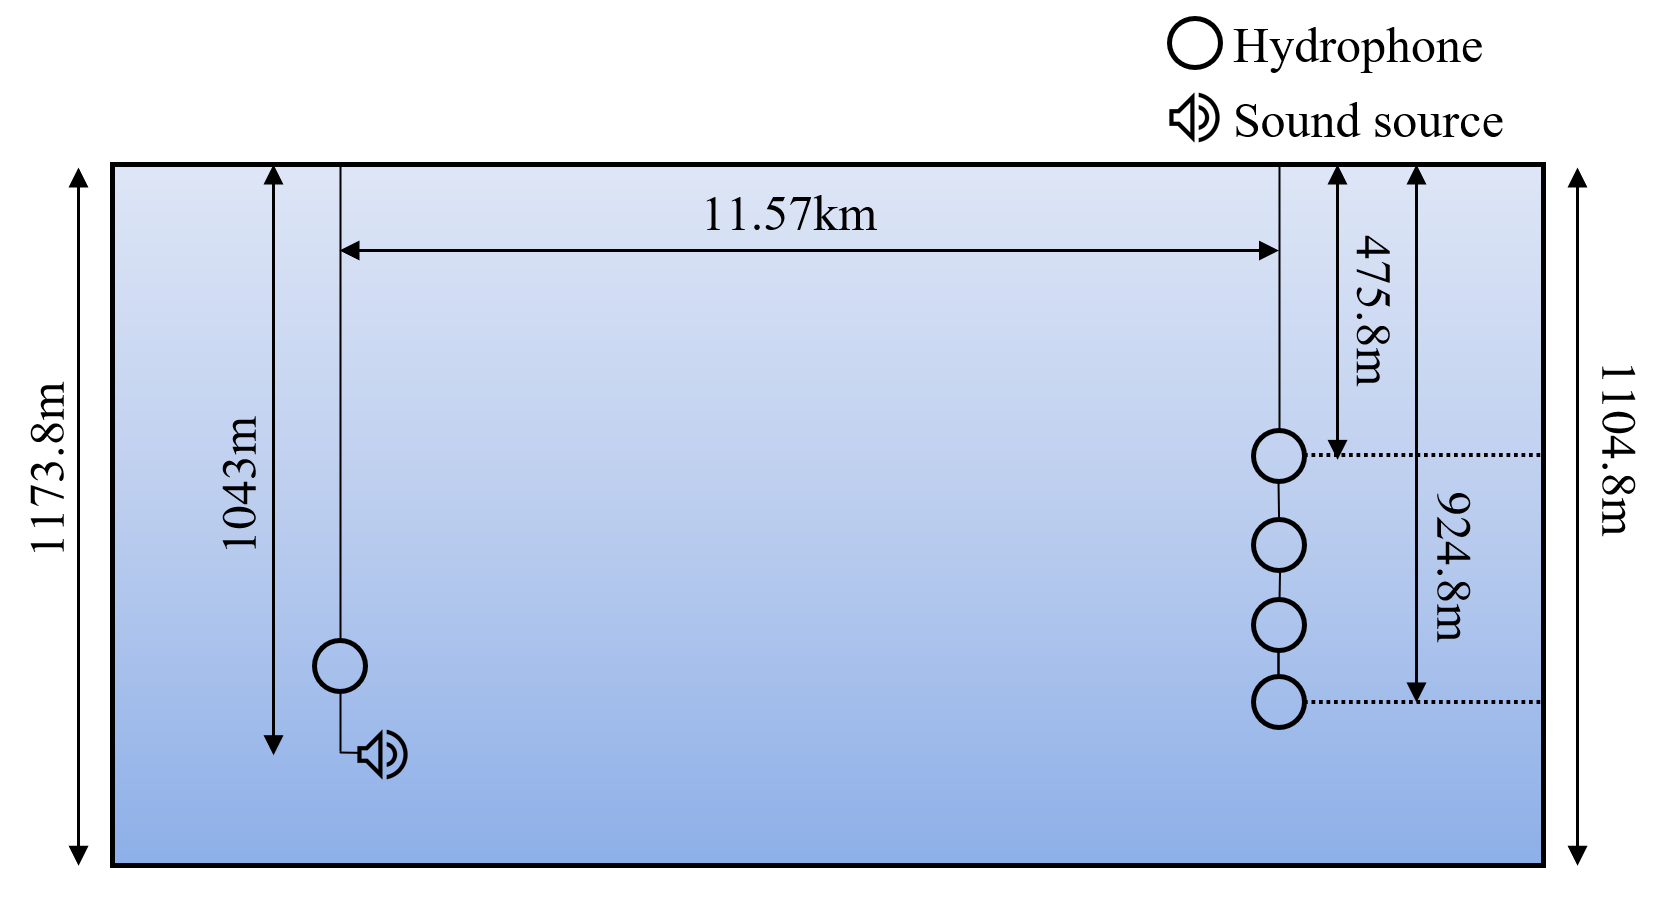
\includegraphics[width=4in]{fig/1setup.png}
\caption{Experimental setup and geometric configuration (schematic). }
\label{fig:geometry}
\end{figure*}

\subsubsection{Sound Speed Profile}

The sound speed profile (SSP) measured during the experiment is shown in Fig.~\ref{fig:ssp}. The profile exhibits a typical deep-ocean structure: a seasonal thermocline extending to approximately 400~m, a main thermocline spanning from 400~m to 950~m, and an underlying deep isothermal layer. The VLA was strategically positioned within this layer (475.8 m to 924.8 m) to capture the acoustic field's evolution and the source was located in this stable deep layer. This geometry is critical because it exposes signals received at each thermocline regime to regime-specific refractive bending—from weak deflection in the upper thermocline, through strong downward refraction in the lower thermocline convergence zone, to near-axial propagation at the thermocline base—thereby producing the thermocline-dependent multipath structures investigated in this work. The sound-channel axis, characterized by minimum sound speed, is located at approximately 950-1000~m depth, below the deepest receiver.

\begin{figure}[!t]
\centering
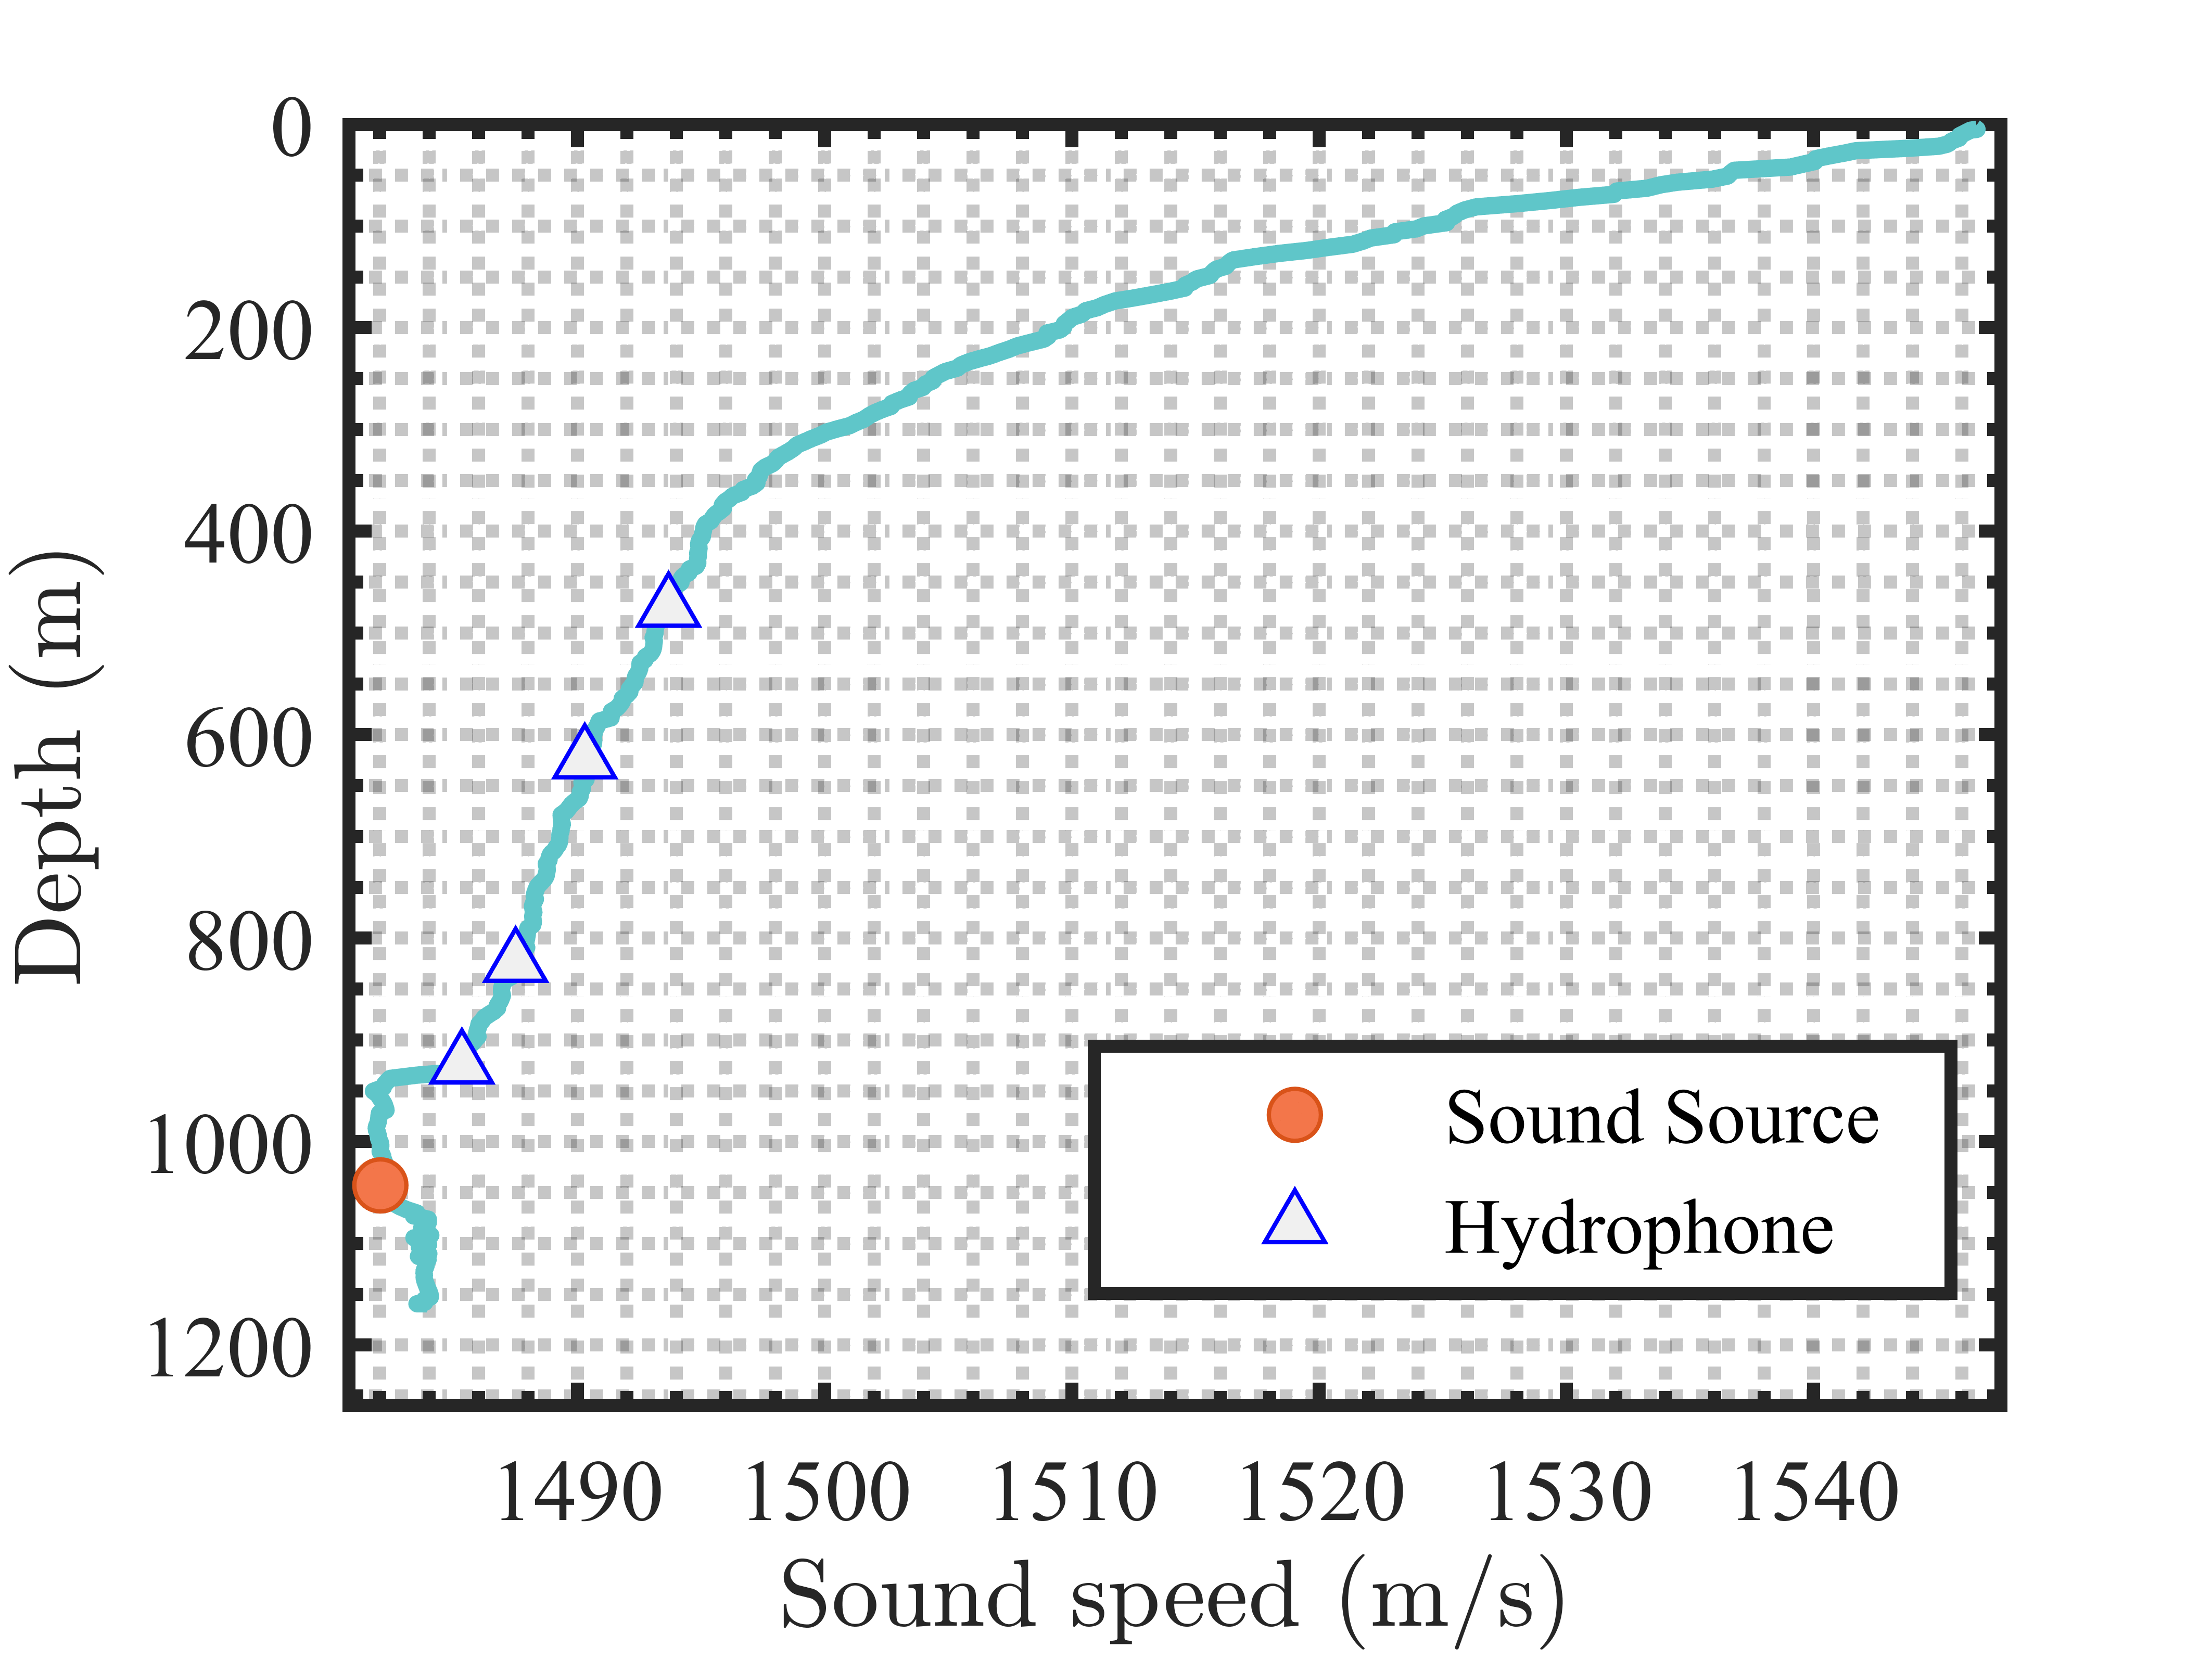
\includegraphics[width=2.5in]{fig/sonic speed2.png}
\caption{Measured sound speed profile (SSP) with transmitter and VLA positions indicated. }
\label{fig:ssp}
\end{figure}

\subsubsection{Probe Signal Design}

The probe signal was designed to balance long range transmission capability and temporal-resolution requirements. To enable accurate channel estimation under significant delay spread (expected to exceed 100~ms) and potential time variation, we used a phase-modulated pseudo-random binary sequence (PRBS). Specifically, an 11th-order maximal-length sequence (M-sequence) with length $L = 2^{11}-1 = 2047$ symbols was used\cite{ref17}. The sequence was modulated onto an 800~Hz carrier using binary phase-shift keying (BPSK). The duration of symbol was set to $T_s = 5$~ms, yielding a signal bandwidth of $B = 400$~Hz and a raw bit rate of 200~bps. This low-frequency, narrowband design pragmatically mitigates severe frequency-dependent attenuation over the 11.57~km propagation range.

Each transmission frame comprised three segments: (i) a preamble including positive-slope linear frequency modulation (LFM), a single-tone sinusoid and a negative-slope LFM for coarse synchronization and Doppler estimation; (ii) a guard interval of 0.5~s; and (iii) a BPSK-modulated M-sequence payload. The complete frame structure and key signal parameters are summarized in Table~\ref{tab:parameters} and illustrated in Fig.~\ref{fig:frame}.

\begin{figure}[!t]
\centering
\subfloat[]{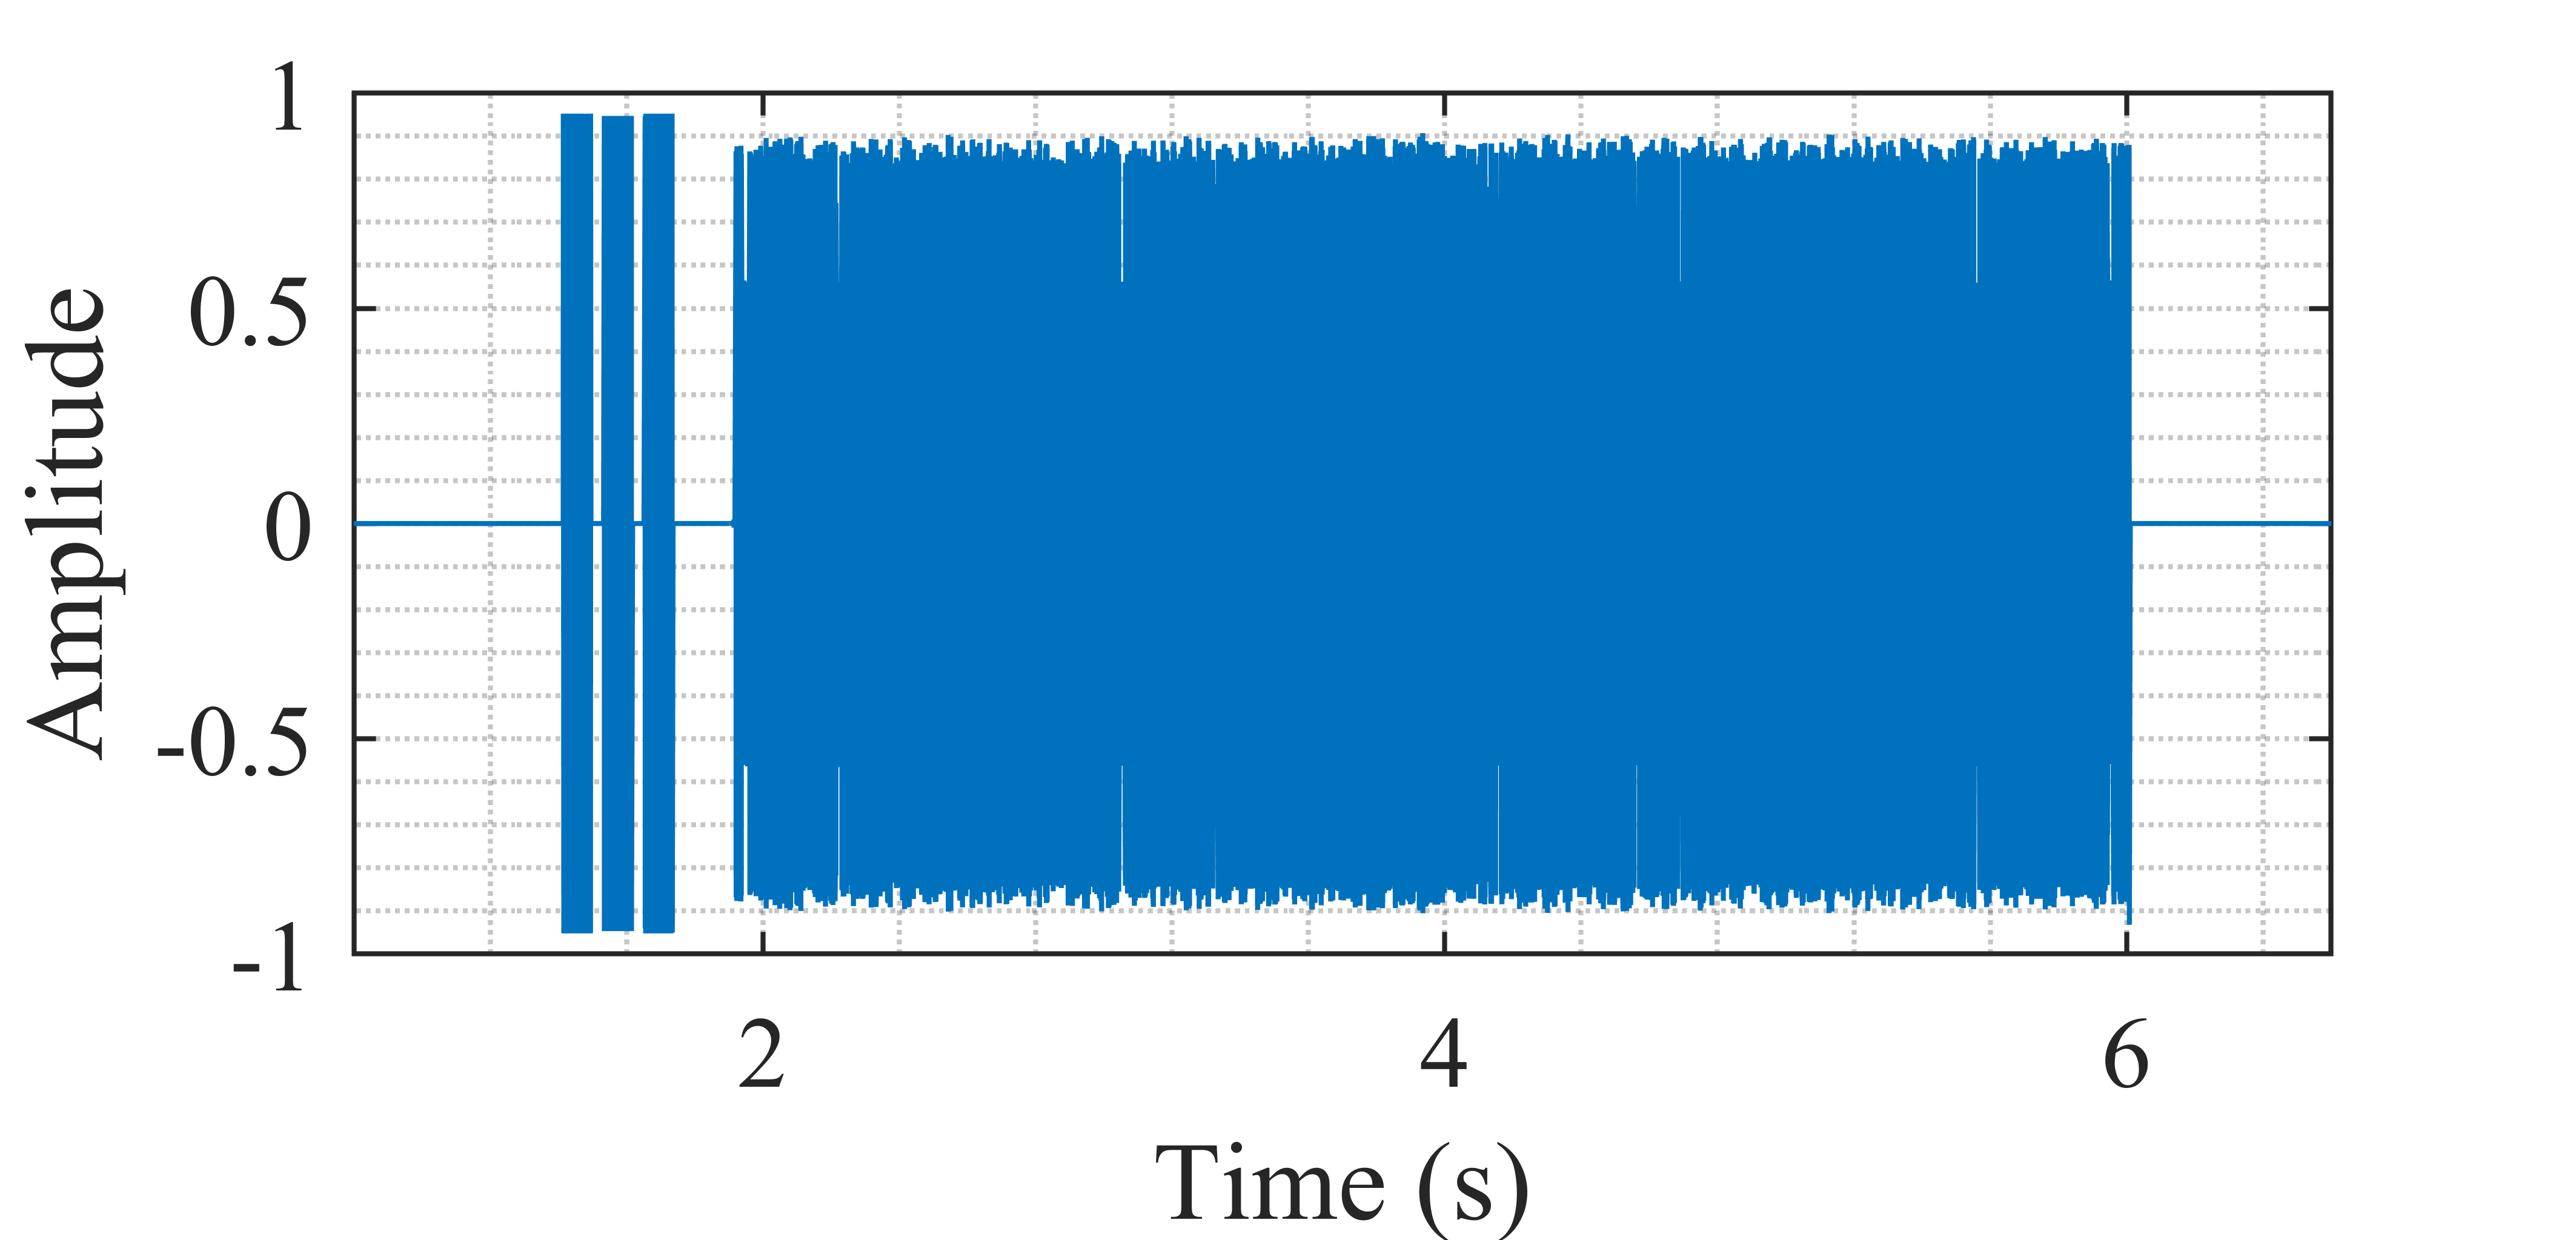
\includegraphics[width=2.5in]{fig/Signal_time.png}
\label{fig_first_case}}
\\
\subfloat[]{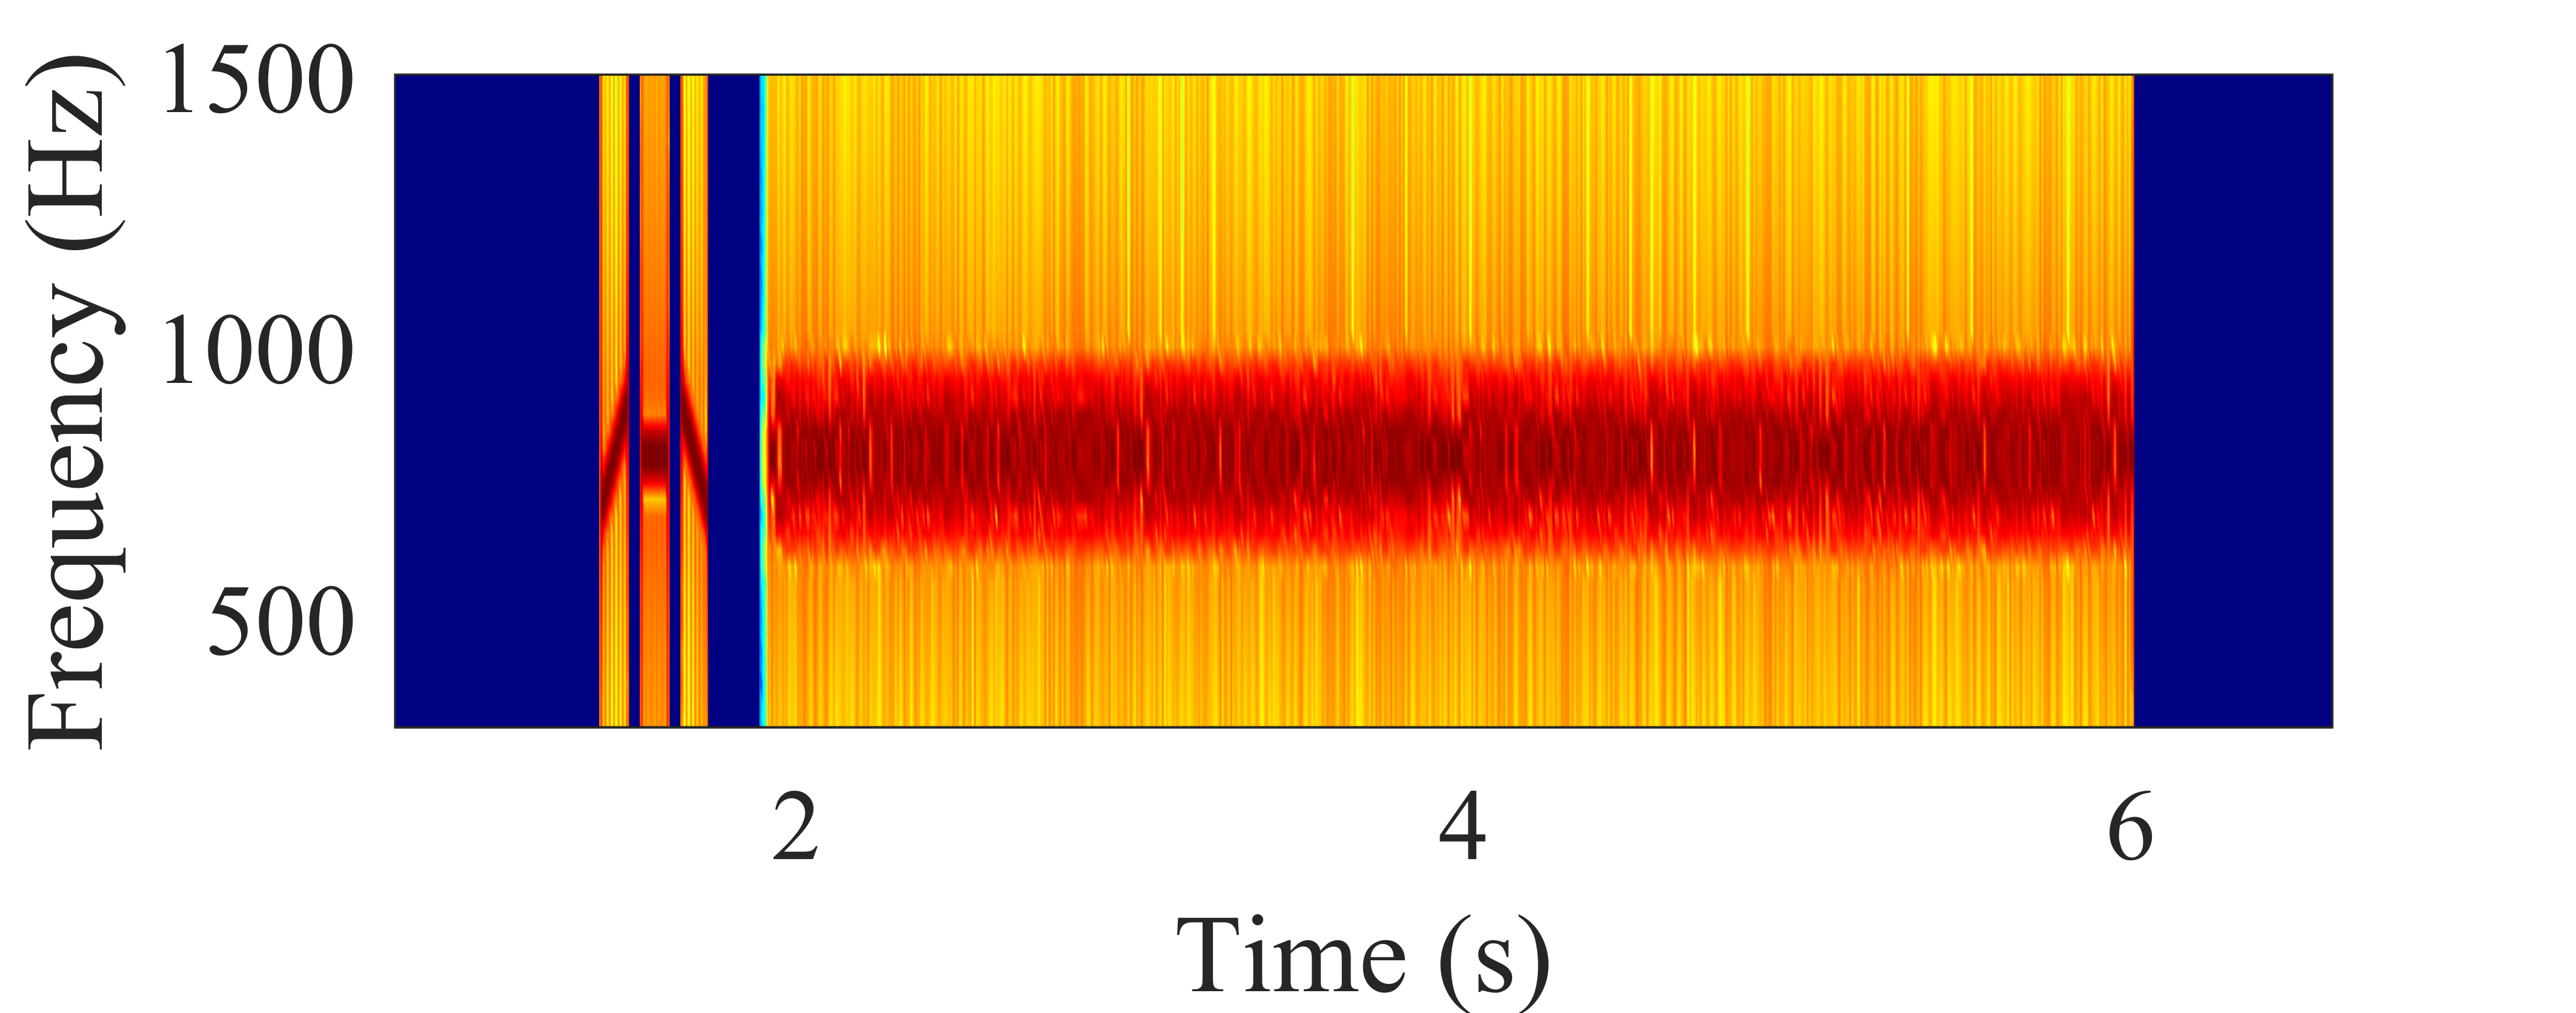
\includegraphics[width=2.5in]{fig/Signal_timefreq.png}
\label{fig_second_case}}
\caption{Frame structure: (a) time-domain waveform, (b) spectrogram.}
\label{fig:frame}
\end{figure}

\begin{table}[!t]
\caption{Key Experimental and Signal Parameters}
\label{tab:parameters}
\centering
\begin{tabular}{lll}
\hline
\textbf{Category} & \textbf{Parameter} & \textbf{Value} \\
\hline
\multirow{4}{*}{\textbf{Geometry}} 
& Transmitter depth & 1043~m \\
& Receiver depths& 475.8, 624.8, 824.8, 924.8~m\\
& Horizontal range & 11.57~km \\
& Water depth (Tx/Rx) & 1173.0~/~1104.8~m \\[2pt]
\multirow{7}{*}{\textbf{Signal}}& Modulation & BPSK \\
& Carrier frequency ($f_c$) & 800~Hz \\
& Bandwidth ($B$) & 400~Hz \\
& Symbol rate & 200~bps \\
& Sequence type & 11th-order M-sequence \\
 & Sequence length & 2047\\
& Sampling rate & 48~kHz \\
\hline
\end{tabular}
\end{table}

\subsection{High-Resolution Time-Varying Channel Estimation}

Accurate estimation of time-varying channel impulse responses (CIRs), denoted as $h(t,\tau)$, in deep sea environments presents a fundamental challenge: balancing the need for long integration intervals, which are essential to provide sufficient processing gain and capture the full delay spread, against the necessity for high temporal resolution needed to track channel dynamics. To address this conflict, we adopt a sliding-window correlation method that decouples these competing requirements.

\subsubsection{Limitations of Conventional Block-Wise Methods}

The conventional approach partitions the received signal into non-overlapping blocks of fixed duration $T_w$, assuming channel stationarity within each block. The CIR of each block is then estimated via cross-correlation with the known probe signal. In our scenario, this creates a critical trade-off: a short $T_w$ improves temporal resolution but yields low correlation-output SNR and may truncate long-delay multipath components; a long $T_w$ improves SNR but blurs temporal variation because the stationarity assumption no longer holds.

Bellhop ray-tracing simulations based on the measured SSP confirm this limitation. Fig.~\ref{fig:fixed_window} shows simulated CIR magnitudes at 475.8~m depth for different $T_w$ values. At $T_w = 1.25$~s, the estimated multipath structure is already severely distorted relative to the benchmark case (no segmentation), indicating that channel coherence time is shorter than the window length required for reliable estimation. At the same time, even this window length still provides insufficient temporal resolution for dynamic tracking.

\begin{figure*}[!t]
\centering
\subfloat[]{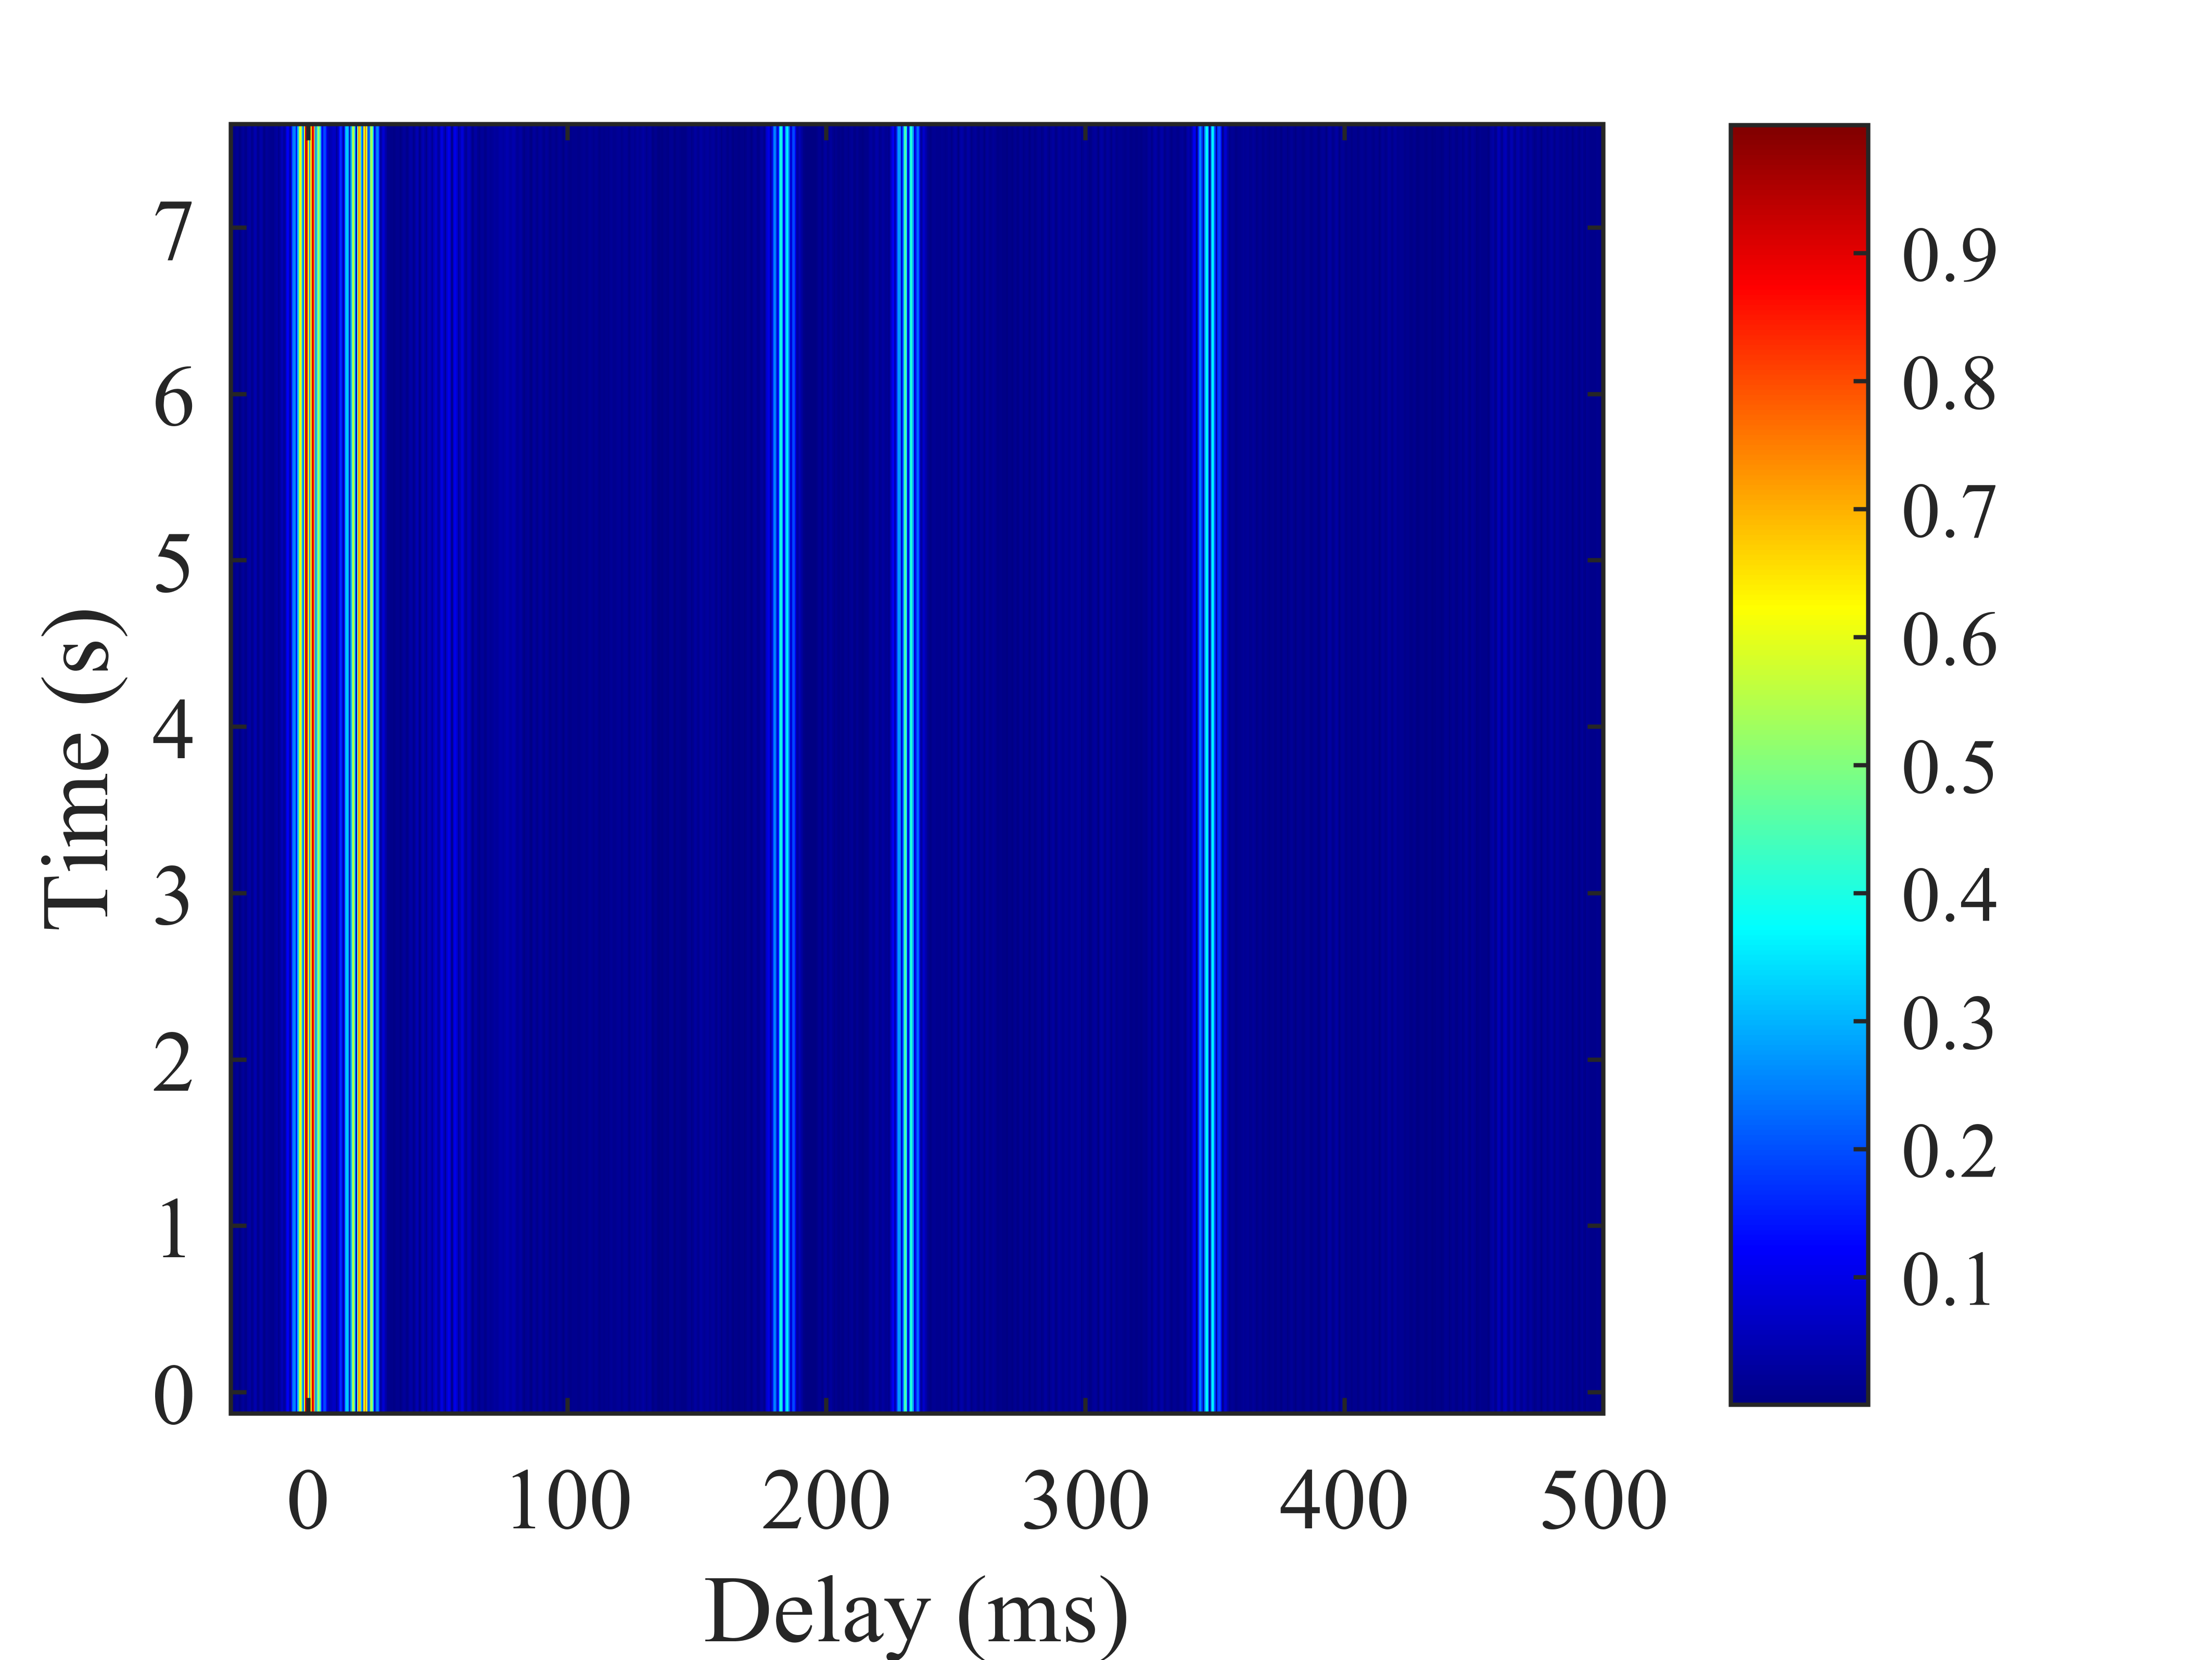
\includegraphics[width=2.5in]{fig/CIR_NoWin.png}
\label{fixed_window_first}}
\hfil
\subfloat[]{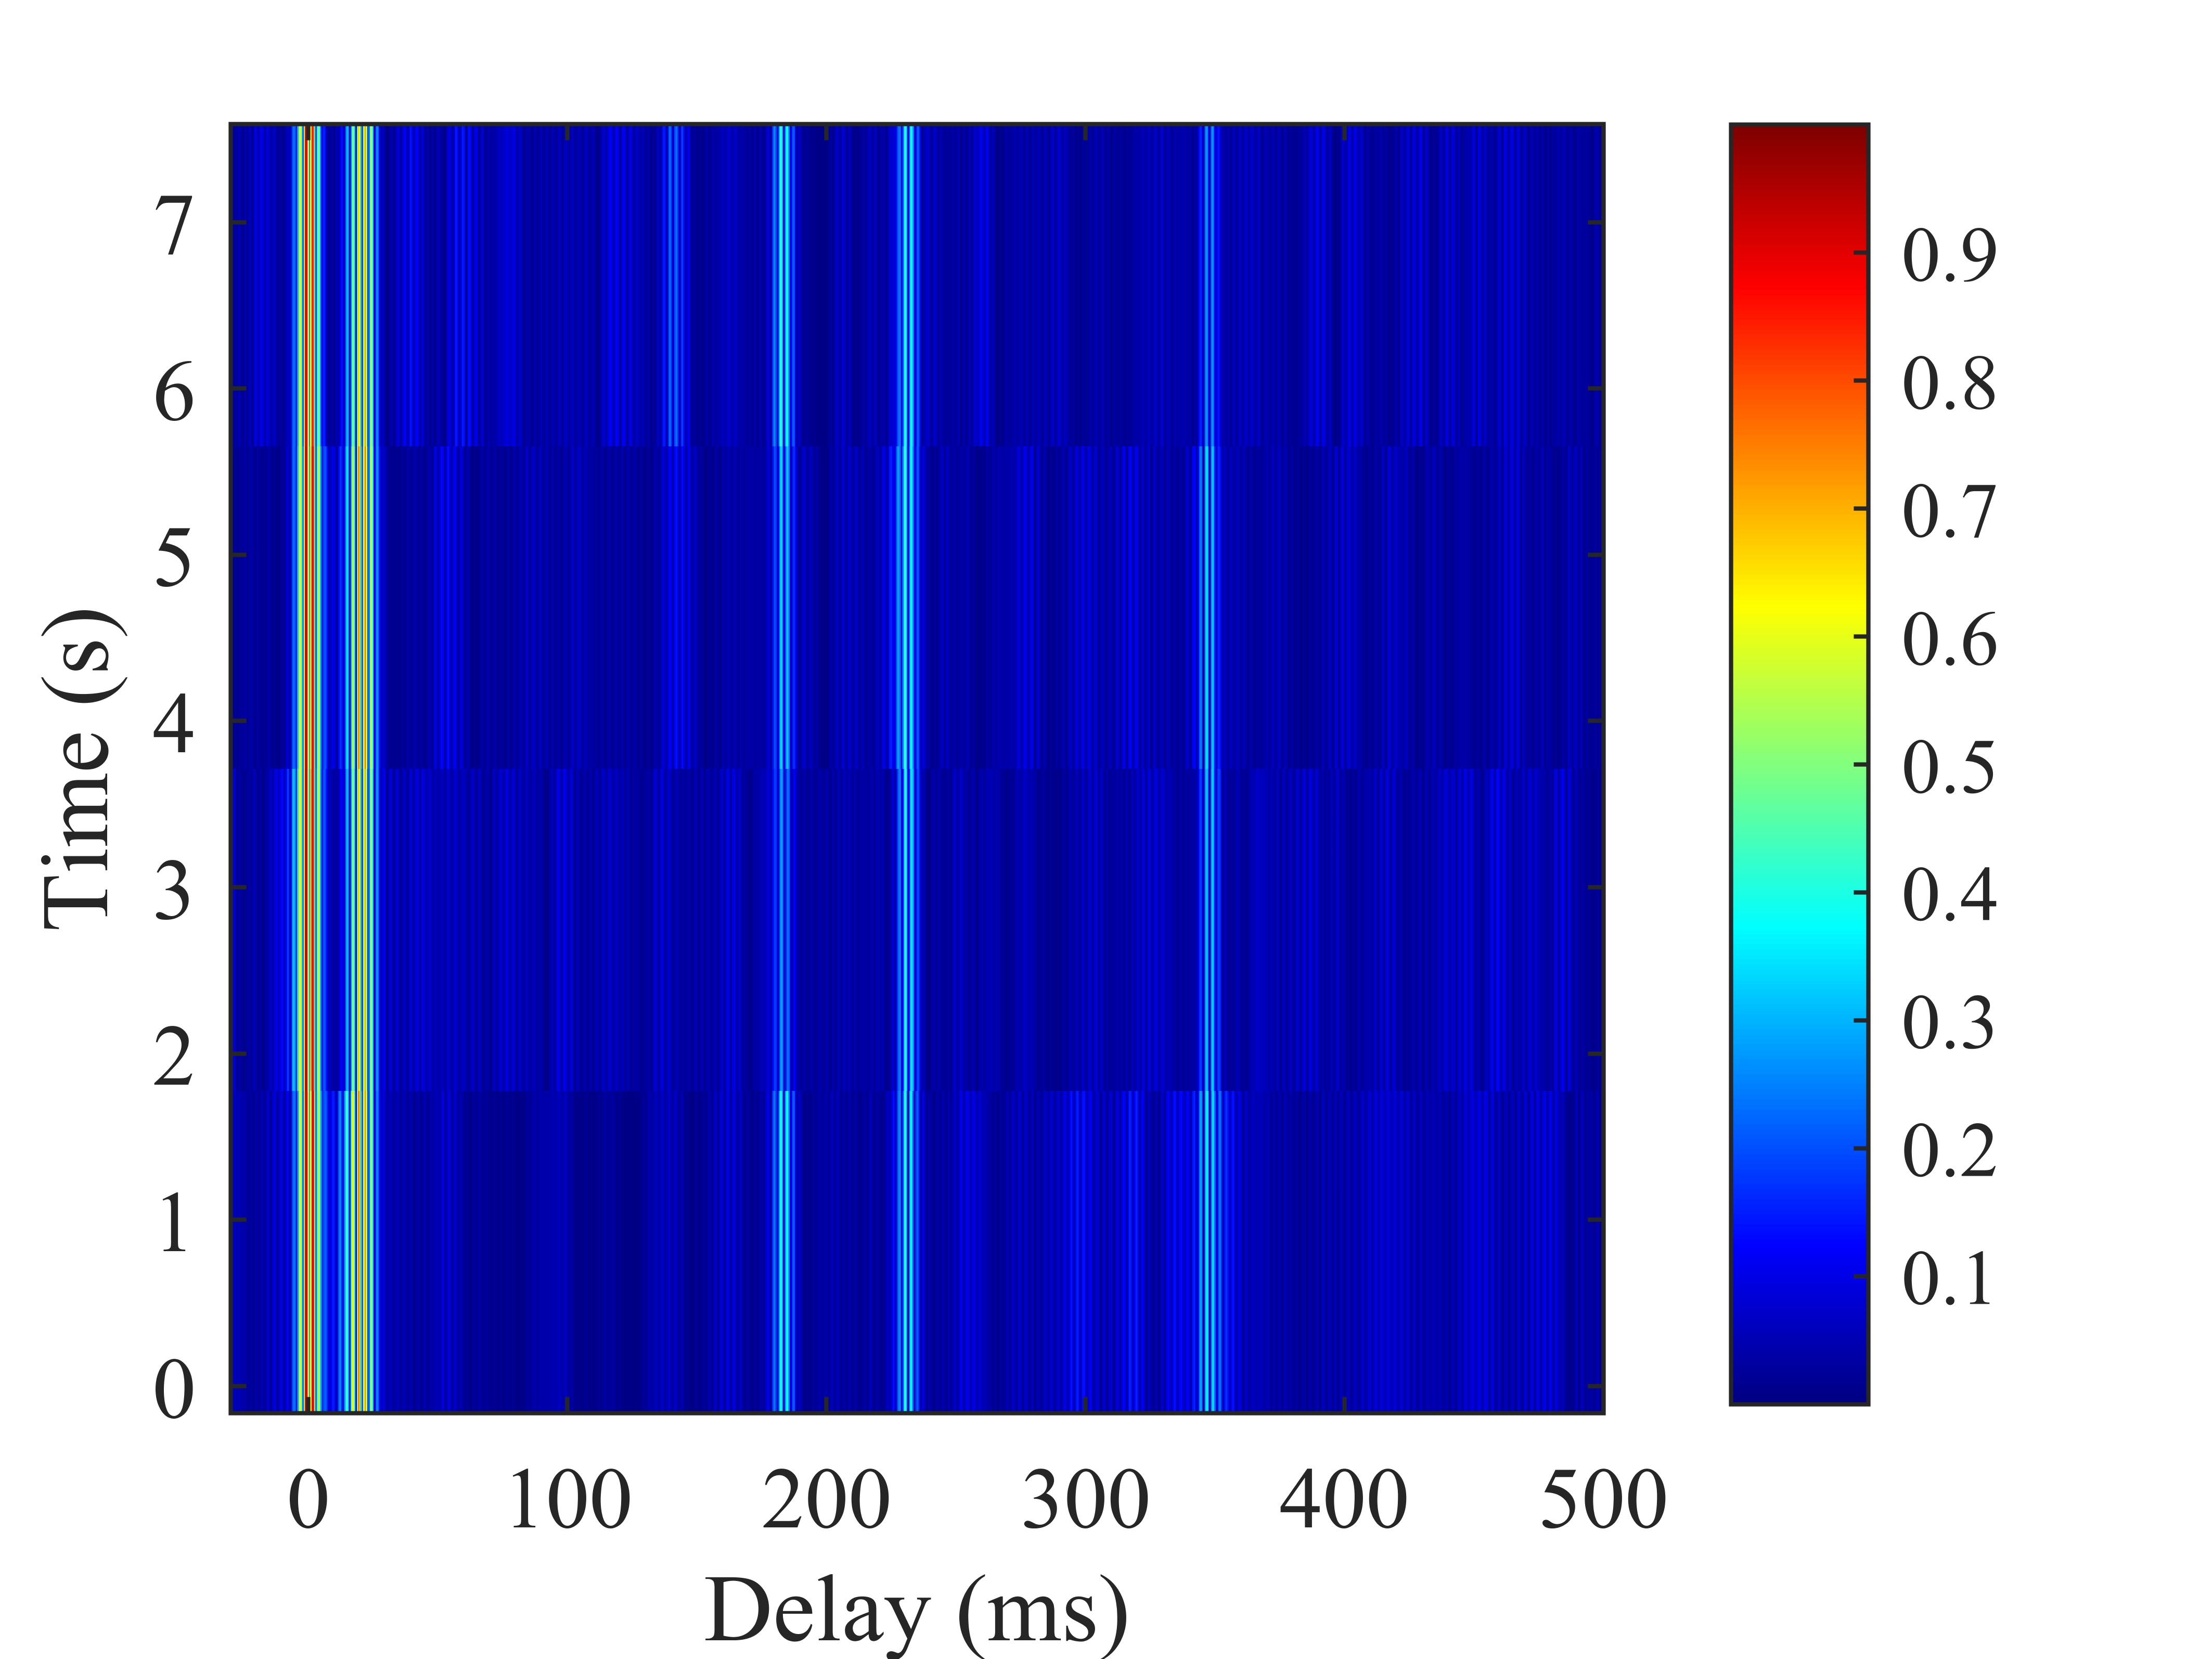
\includegraphics[width=2.5in]{fig/CIR_2.5.png}
\label{fixed_window_second}}
\\
\subfloat[]{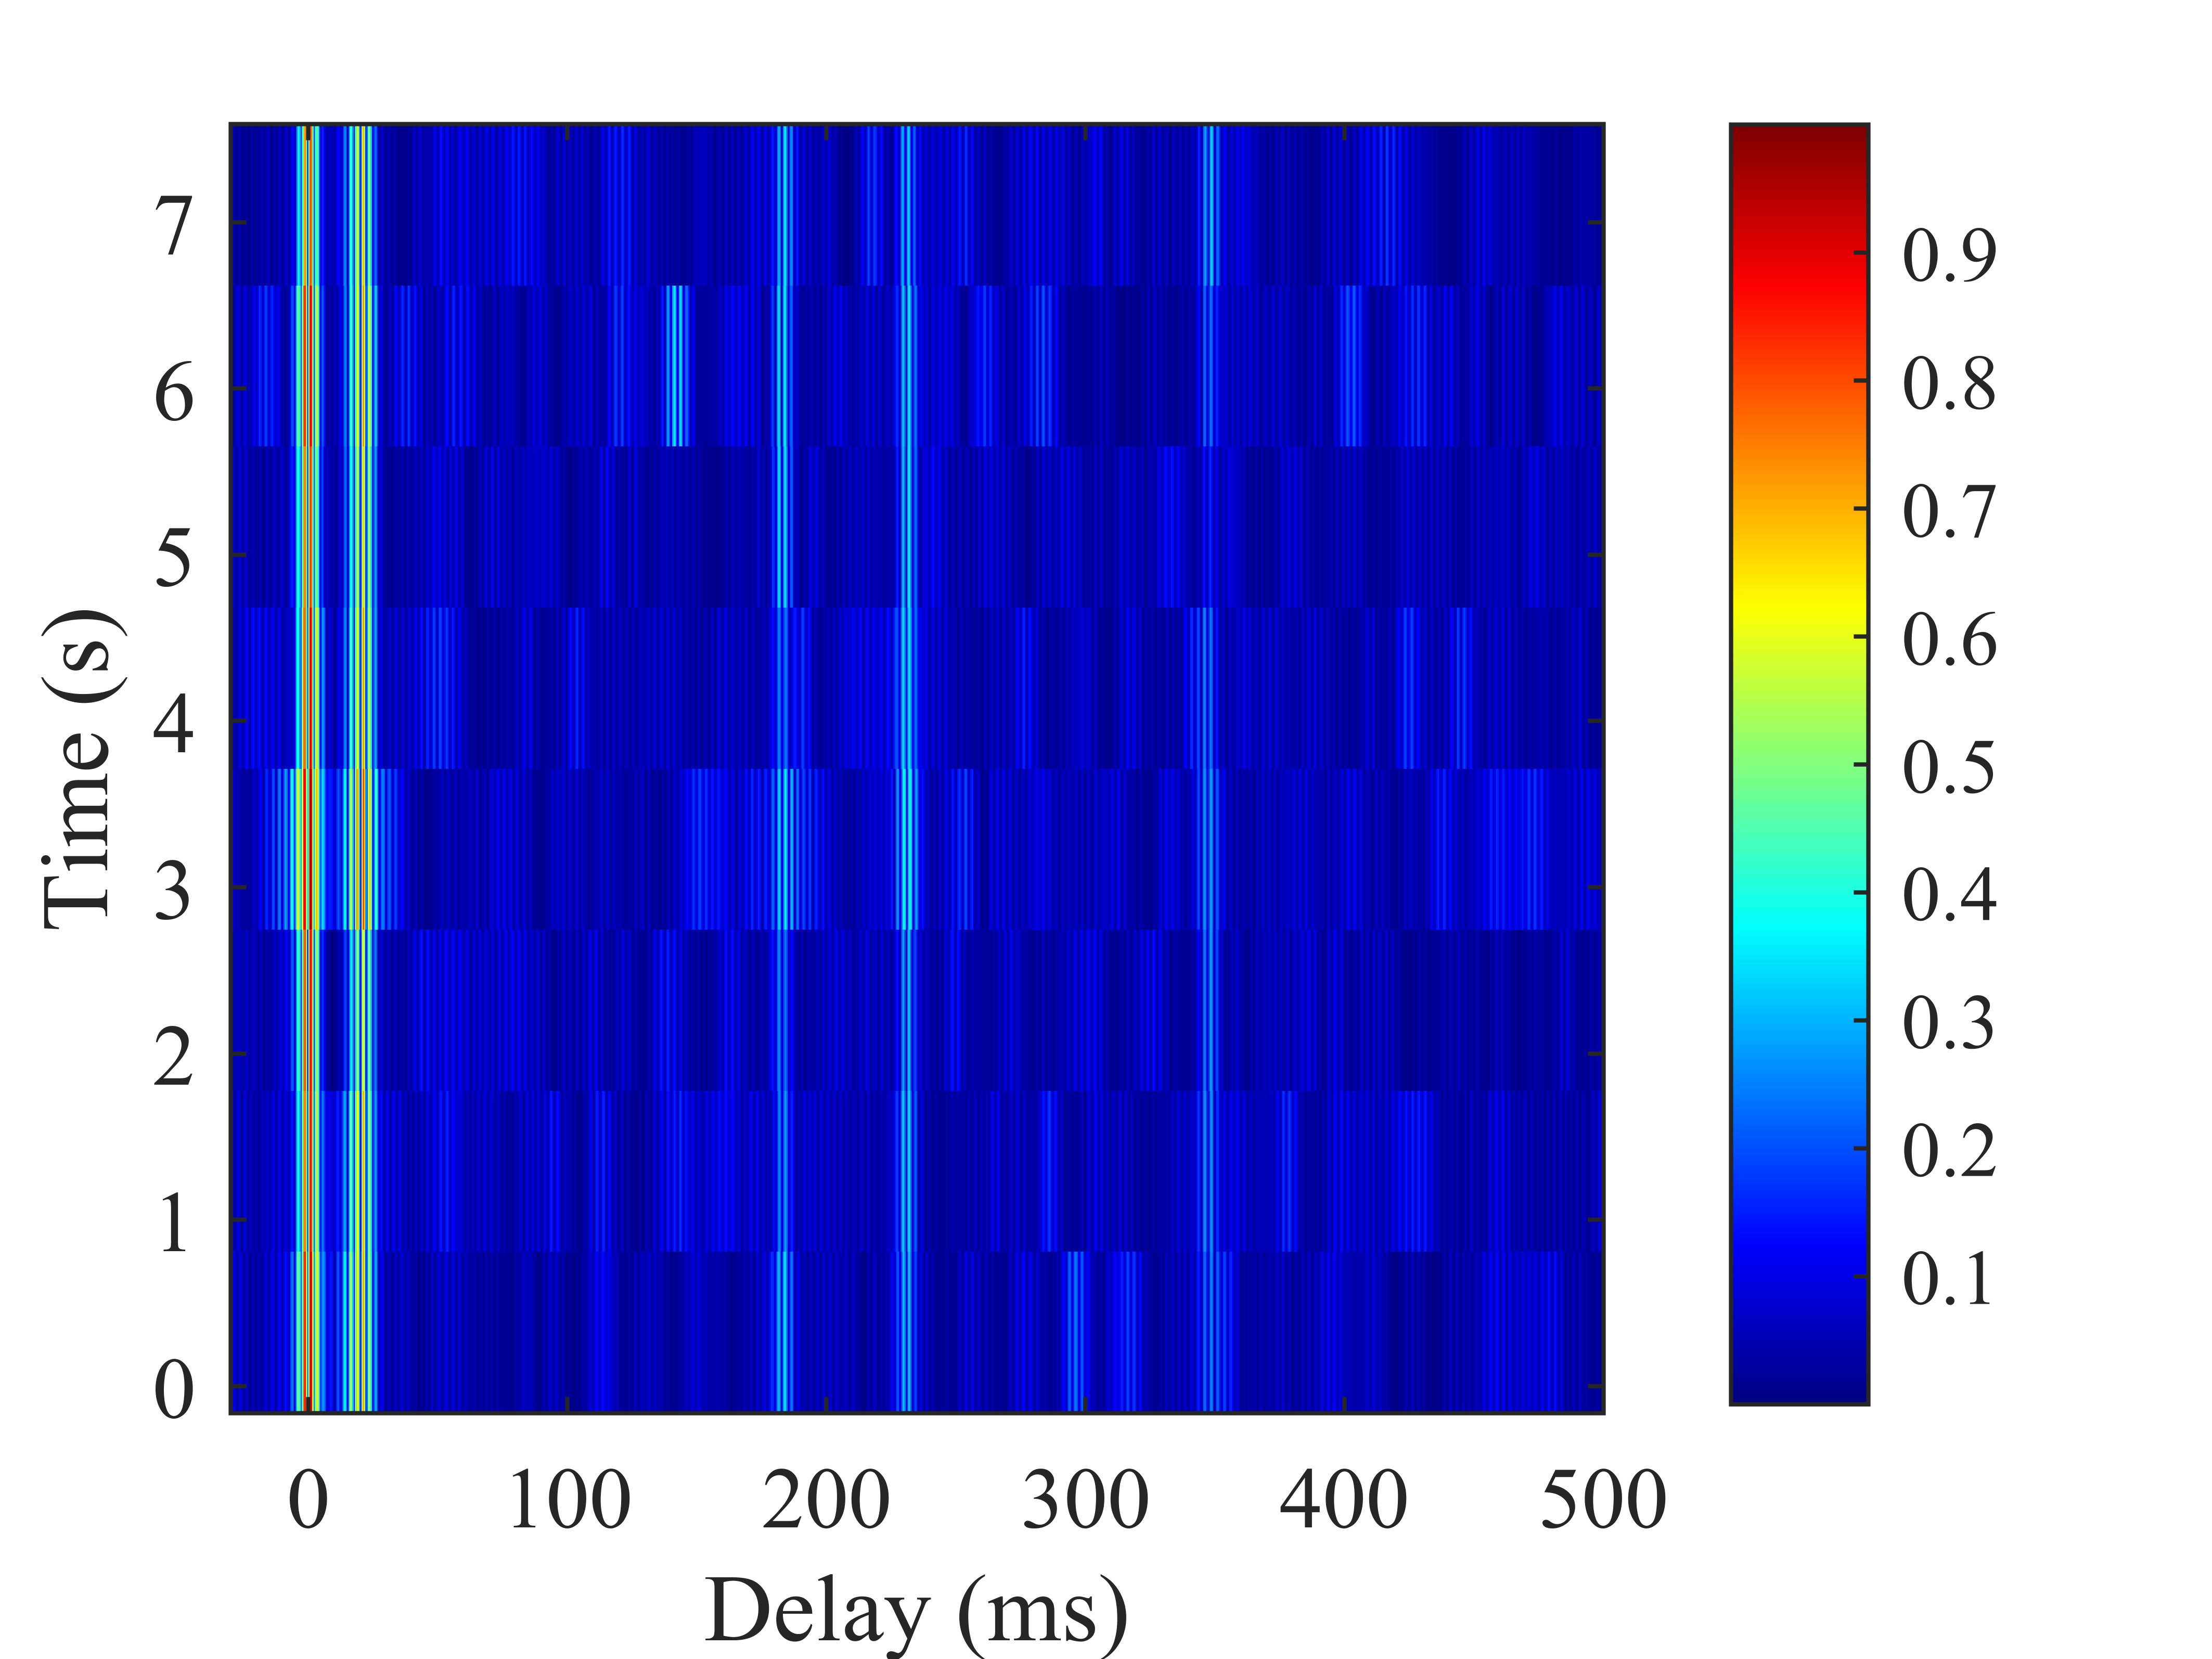
\includegraphics[width=2.5in]{fig/CIR_1.25.png}
\label{fixed_window_third}}
\hfil
\subfloat[]{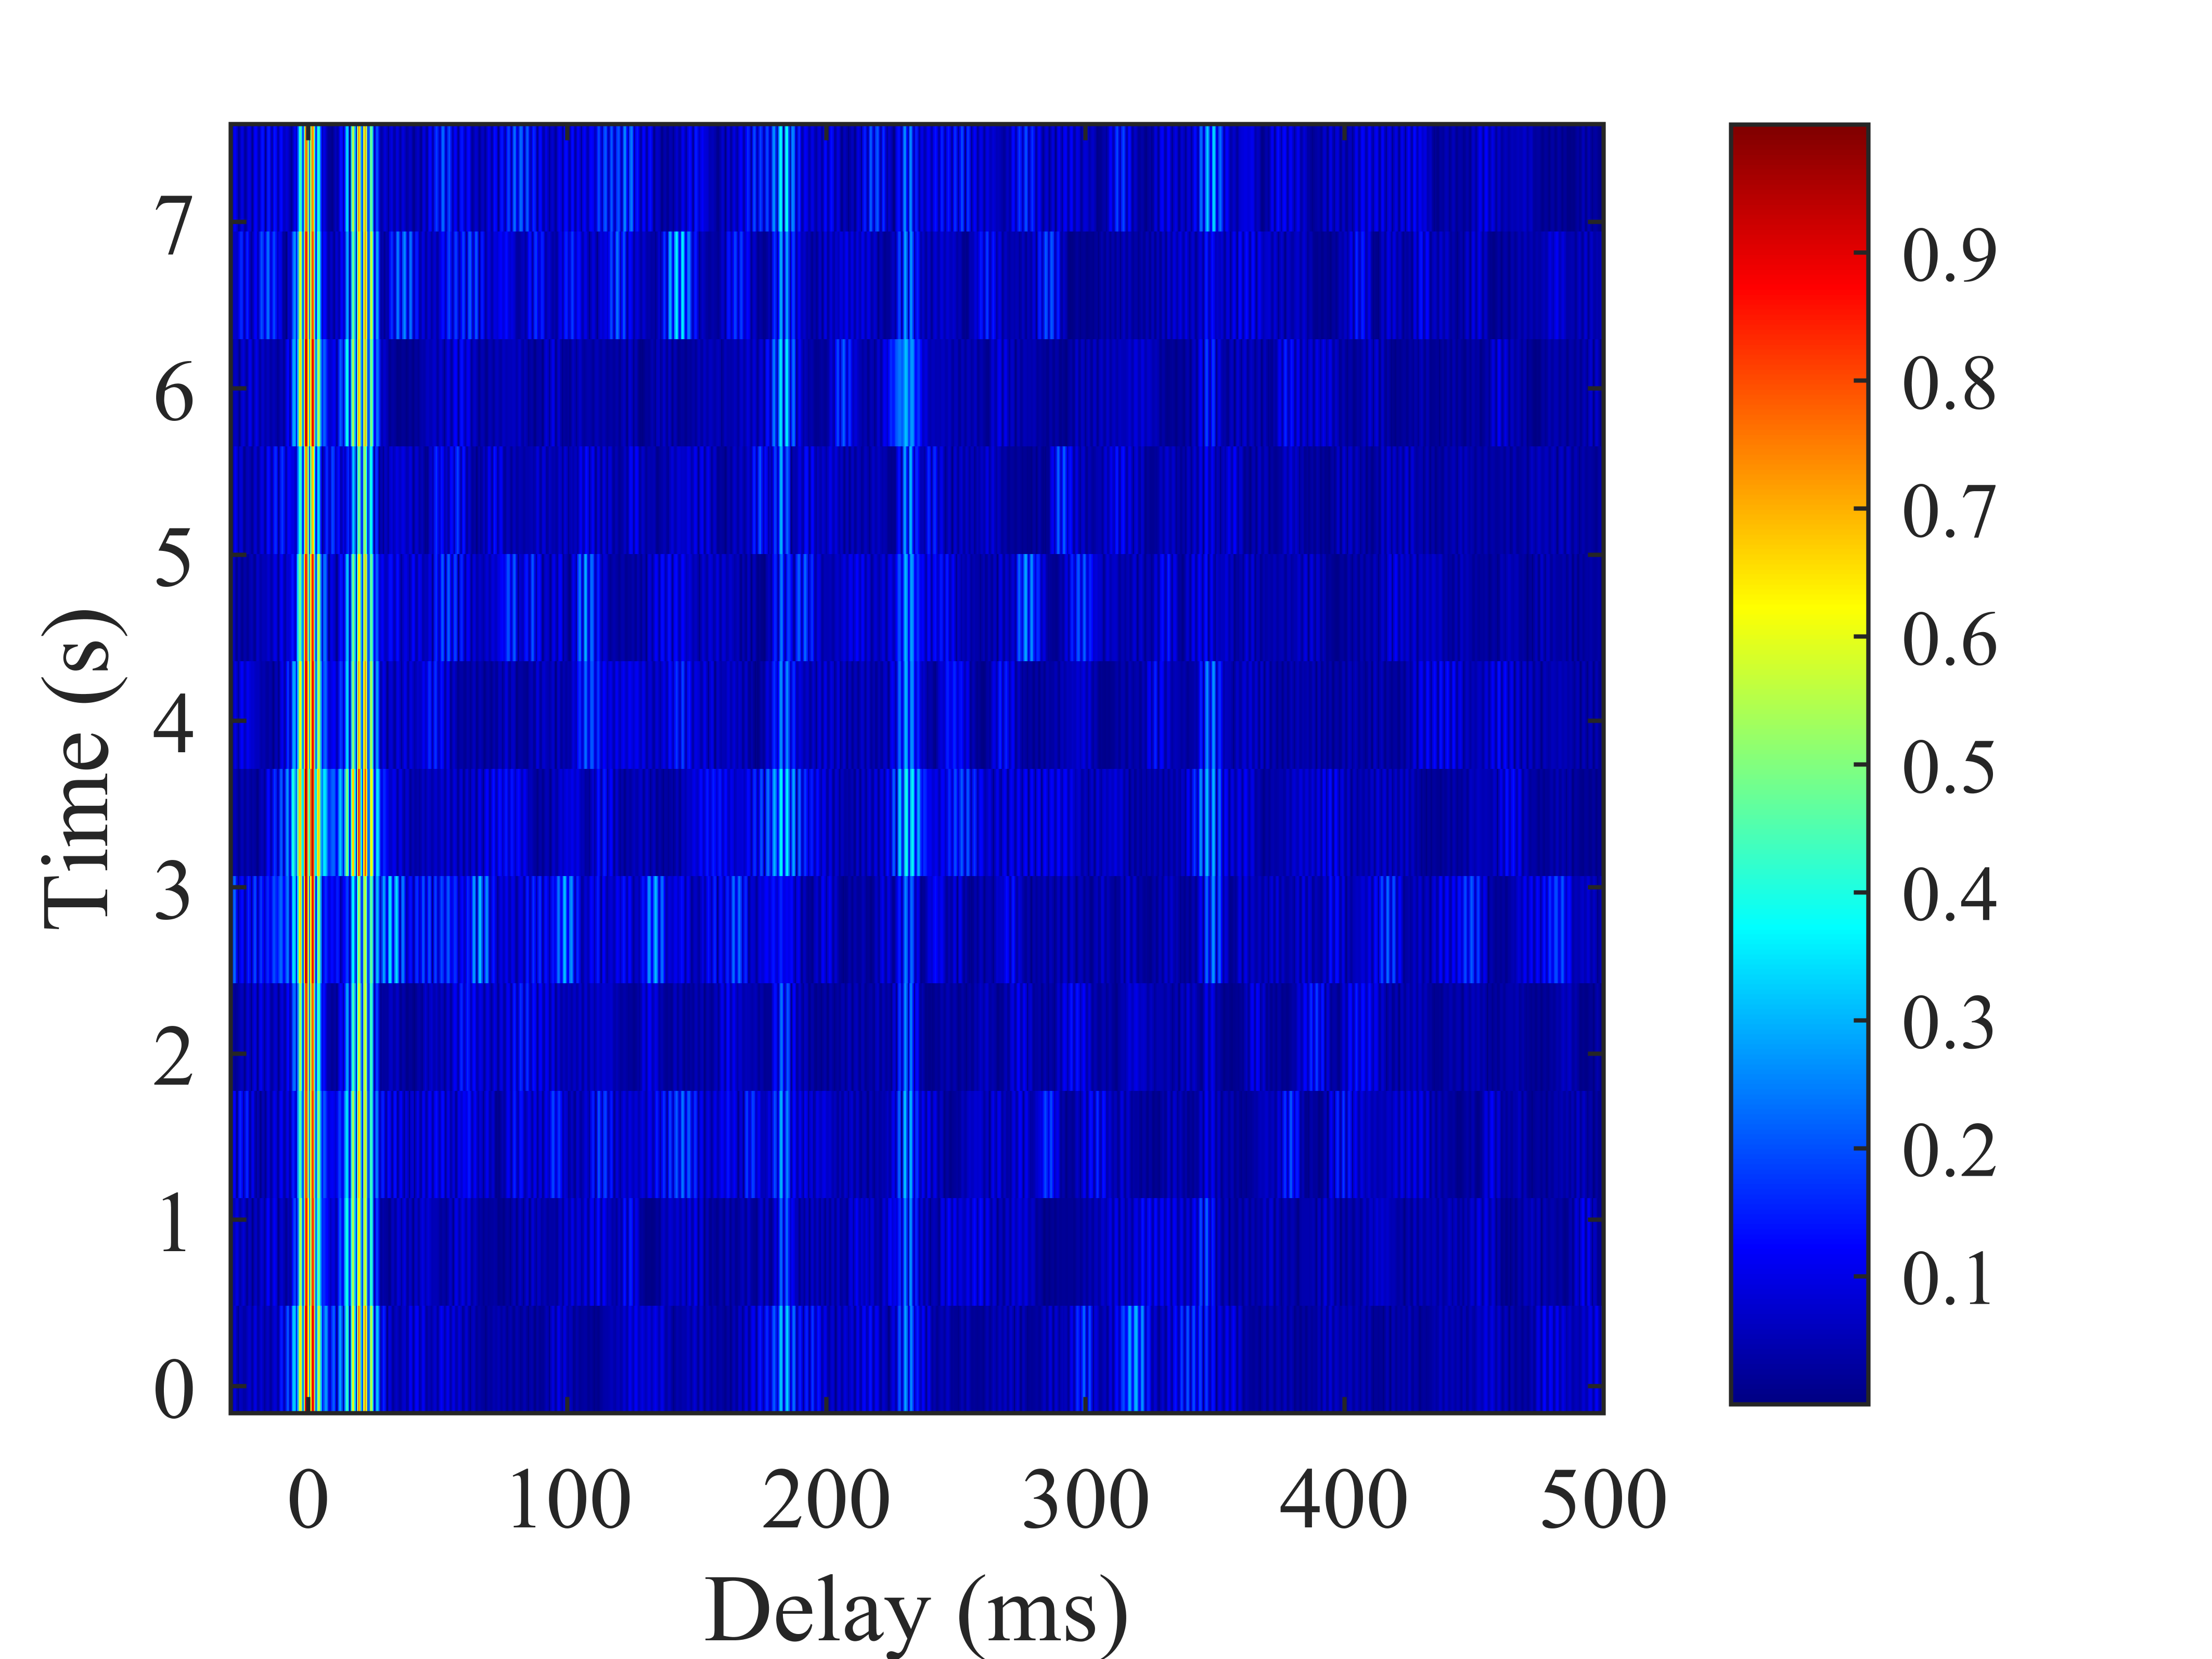
\includegraphics[width=2.5in]{fig/CIR_0.625.png}
\label{fixed_window_forth}}
\caption{Fixed-window channel estimation degradation at 475.8~m depth: (a) reference CIR without windowing; (b)--(d) estimated CIRs with $T_w = 2.5$~s, 1.25~s, and 0.625~s, respectively.}
\label{fig:fixed_window}
\end{figure*}

\subsubsection{Sliding-Window Correlation Method}

To resolve this conflict, we employ a sliding-window correlation technique that decouples the integration length from the temporal sampling interval. Let $\mathbf{x}[n]$ and $\mathbf{y}[n]$ denote discrete-time synchronized transmit and receive sequences, respectively. A rectangular window $\mathbf{w}[n]$ of length $L_w$ samples is defined as:
\begin{equation}
\mathbf{w}[n] = \begin{cases} 
1, & 0 \leq n \leq L_w - 1 \\
0, & \text{otherwise}
\end{cases}
\end{equation}

The window slides along the time axis with step size $S$ samples, generating $K$ overlapping segments. The $k$-th windowed signals are:
\begin{align}
\mathbf{x}_k[n] &= \mathbf{x}[n + kS] \cdot \mathbf{w}[n], \\
\mathbf{y}_k[n] &= \mathbf{y}[n + kS] \cdot \mathbf{w}[n],
\end{align}
for $0 \leq n \leq L_w - 1$ and $k = 0, 1, \ldots, K-1$.

The local CIR estimate at position $k$ is obtained by cross-correlation:
\begin{equation}
\hat{\mathbf{h}}_k[\tau] = \sum_{m=0}^{L_w-1} \mathbf{y}_k[m+\tau] \cdot \mathbf{x}_k^*[m]
\label{eq:sliding_correlation}
\end{equation}

Repeating this process yields a time-varying channel matrix $\mathbf{H} = [\hat{\mathbf{h}}_0, \hat{\mathbf{h}}_1, \ldots, \hat{\mathbf{h}}_{K-1}]^{\mathrm{T}}$ with high temporal fidelity. This framework allows independent parameter optimization: $L_w$ can be set sufficiently large to ensure robust correlation gain and full delay-spread coverage, while $S$ can be set small to enable fine-grained tracking of channel variation.

\subsubsection{Parameter Selection via Simulation}

The selection of $(L_w, S)$ is critical and was determined through systematic Bellhop-based simulations. As shown in Fig.~\ref{fig:parameter_opt}, we evaluated the fidelity of the CIR estimation for different combinations of parameters against a reference case (no windowing). The analysis established quantitative thresholds: a window length $L_w \geq 3$~s is required to maintain near-optimal correlation gain and capture full multipath spread, whereas a step size $S \leq 0.1$~s is required to track channel dynamics without significant temporal aliasing.

\begin{figure*}[!t]
\centering
\subfloat[]{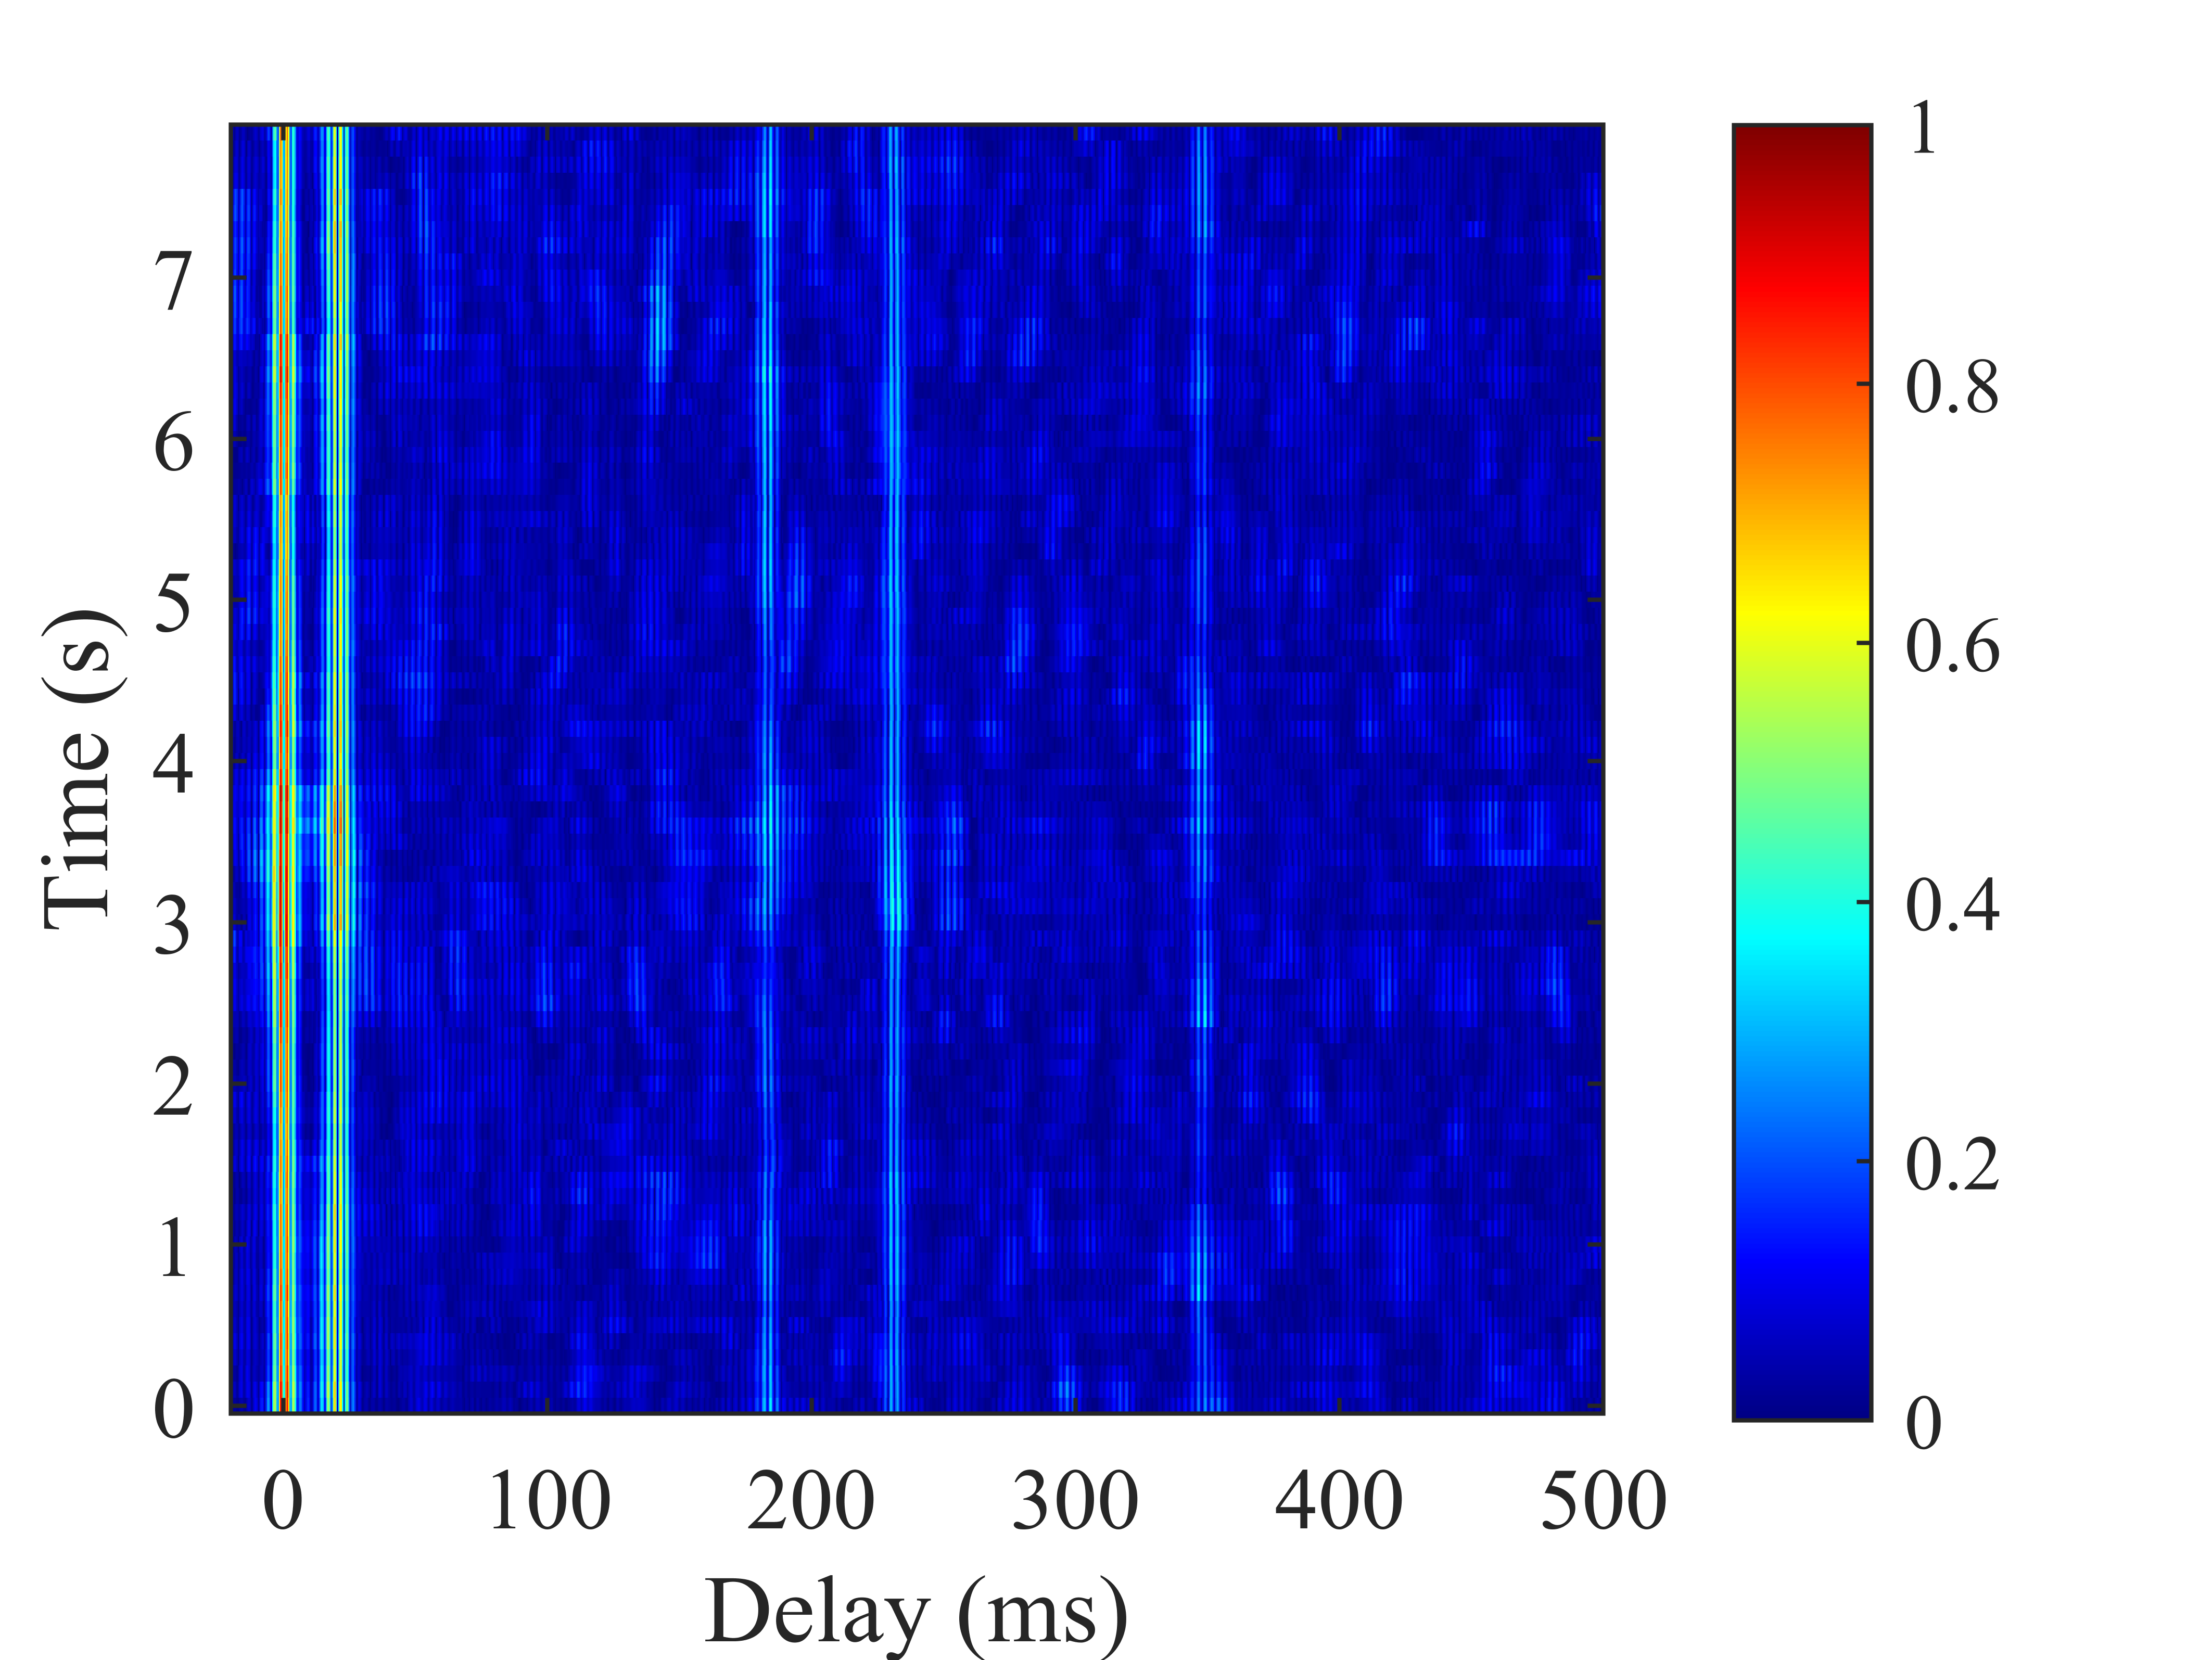
\includegraphics[width=2.5in]{fig/step0.1_window1.png}
\label{parameter_opt_first}}
\hfil
\subfloat[]{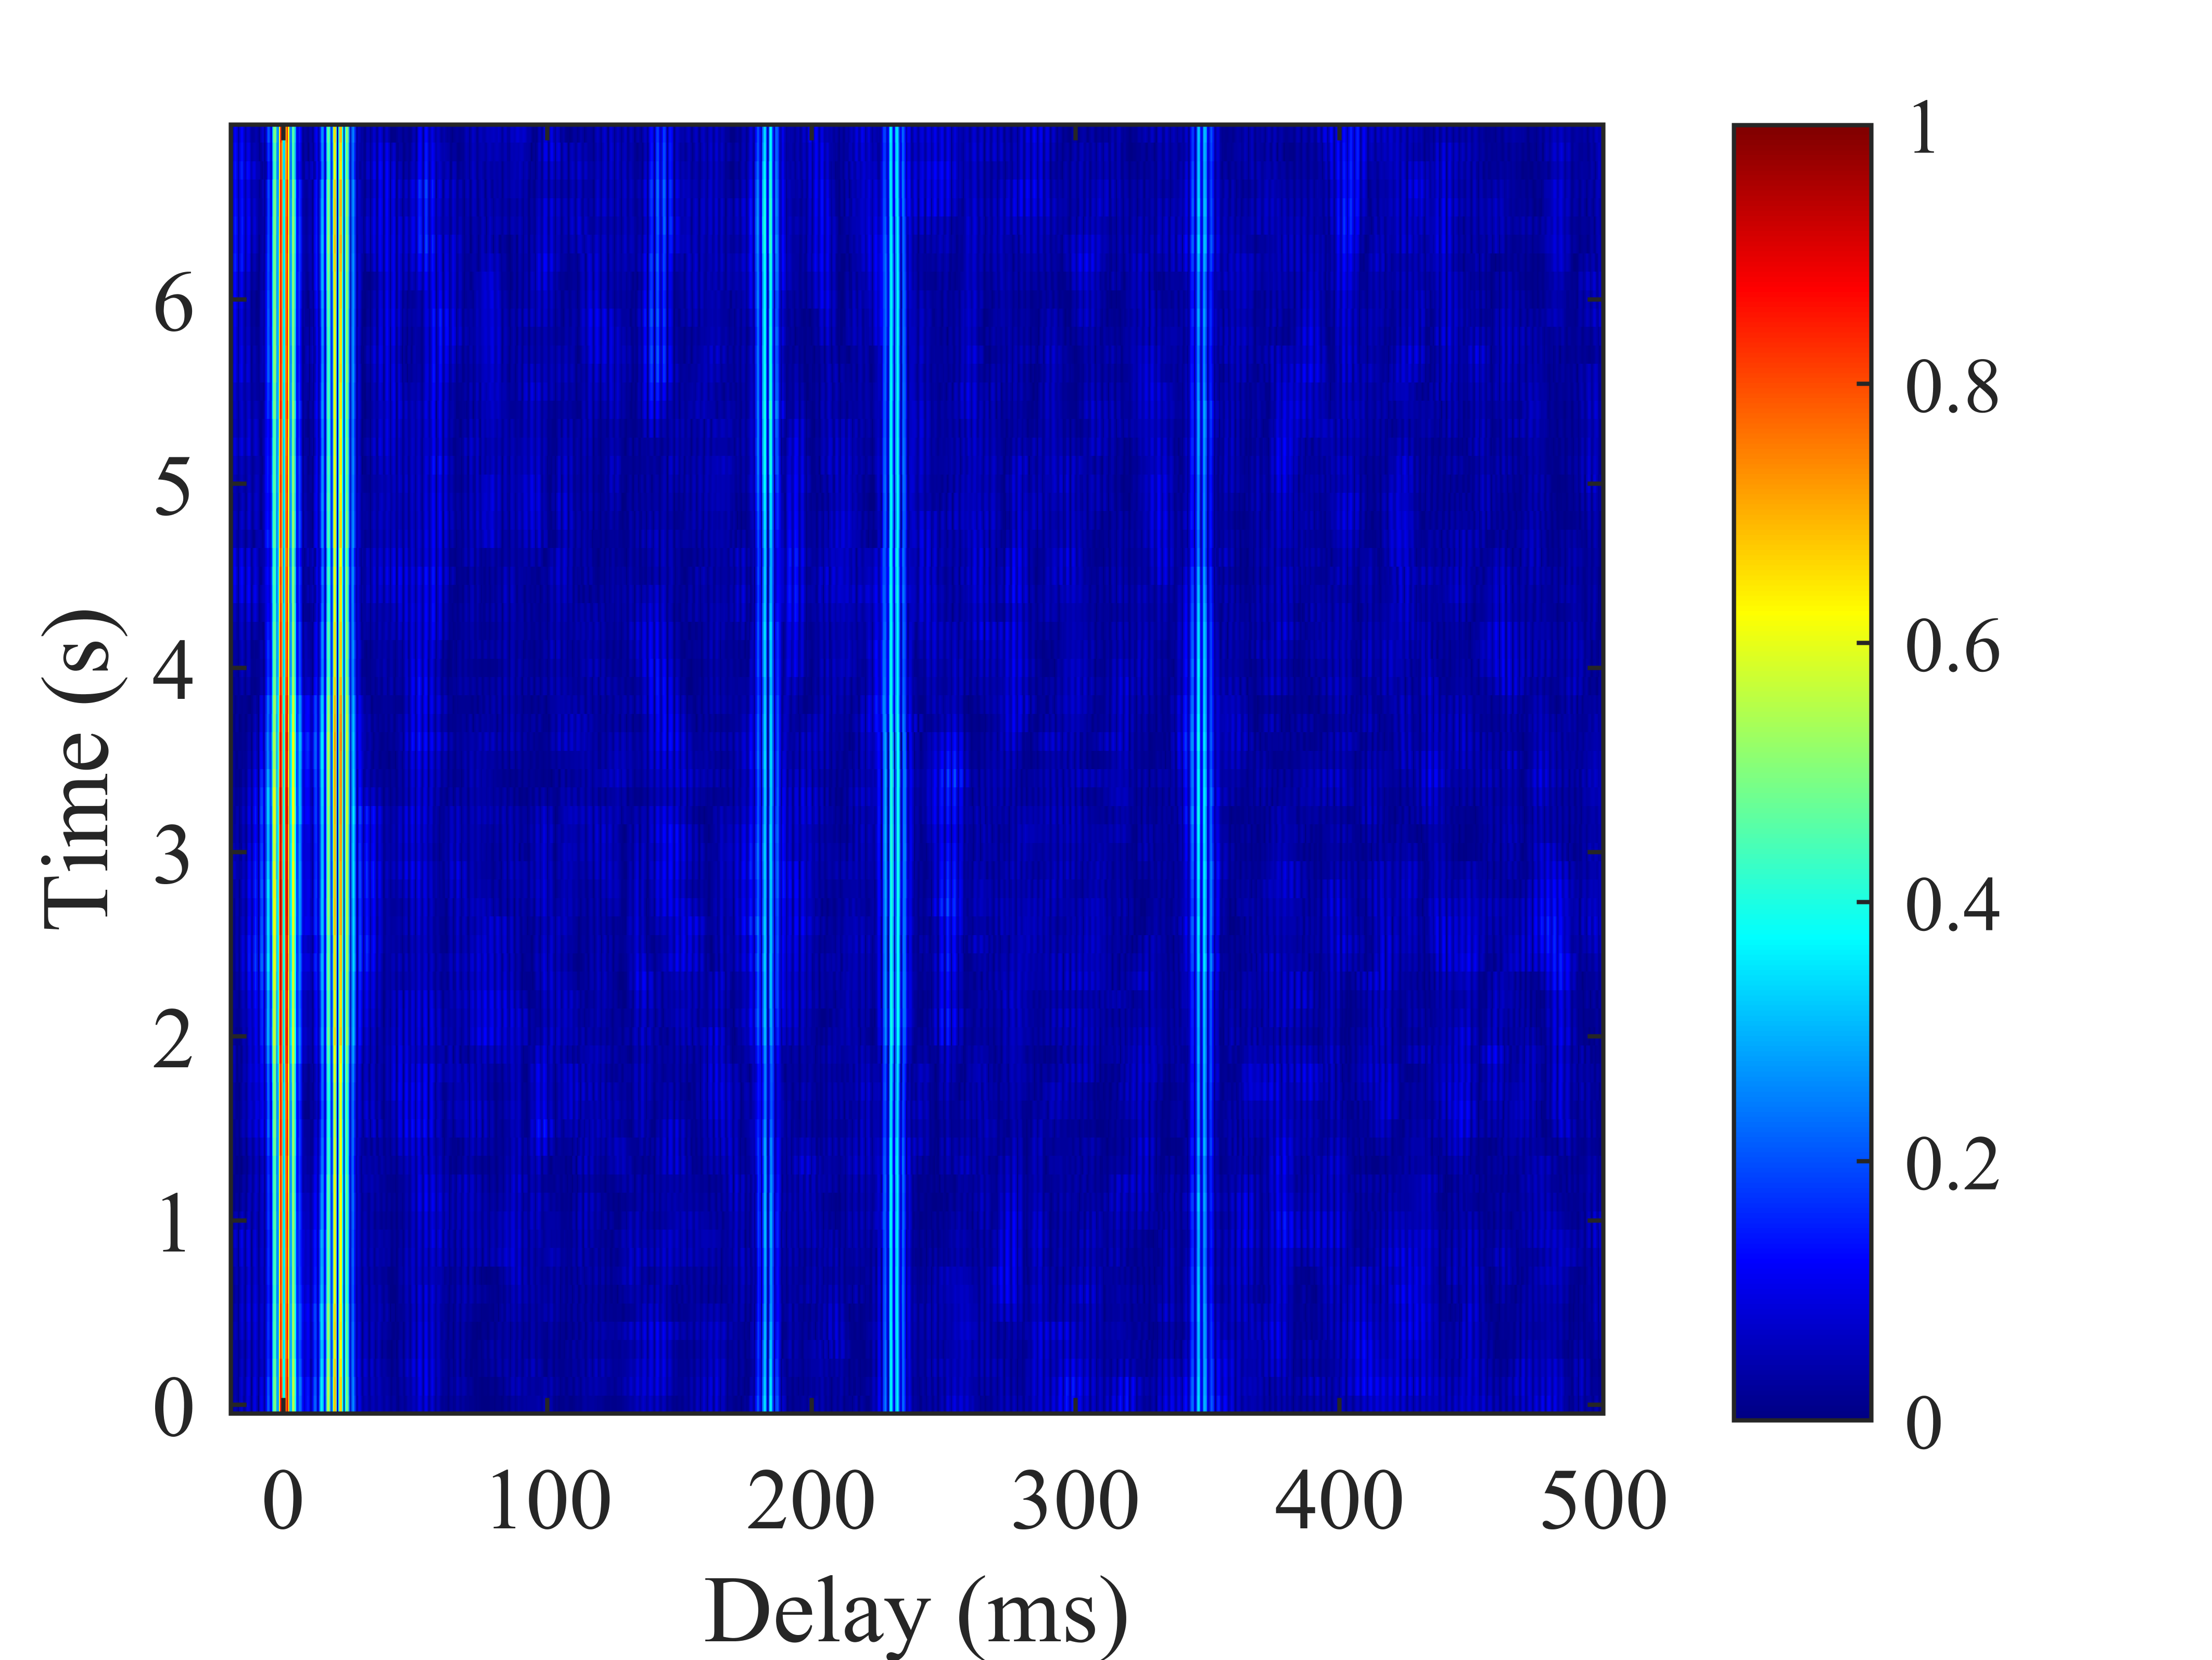
\includegraphics[width=2.5in]{fig/step0.1_window2.png}
\label{parameter_opt_second}}
\\
\subfloat[]{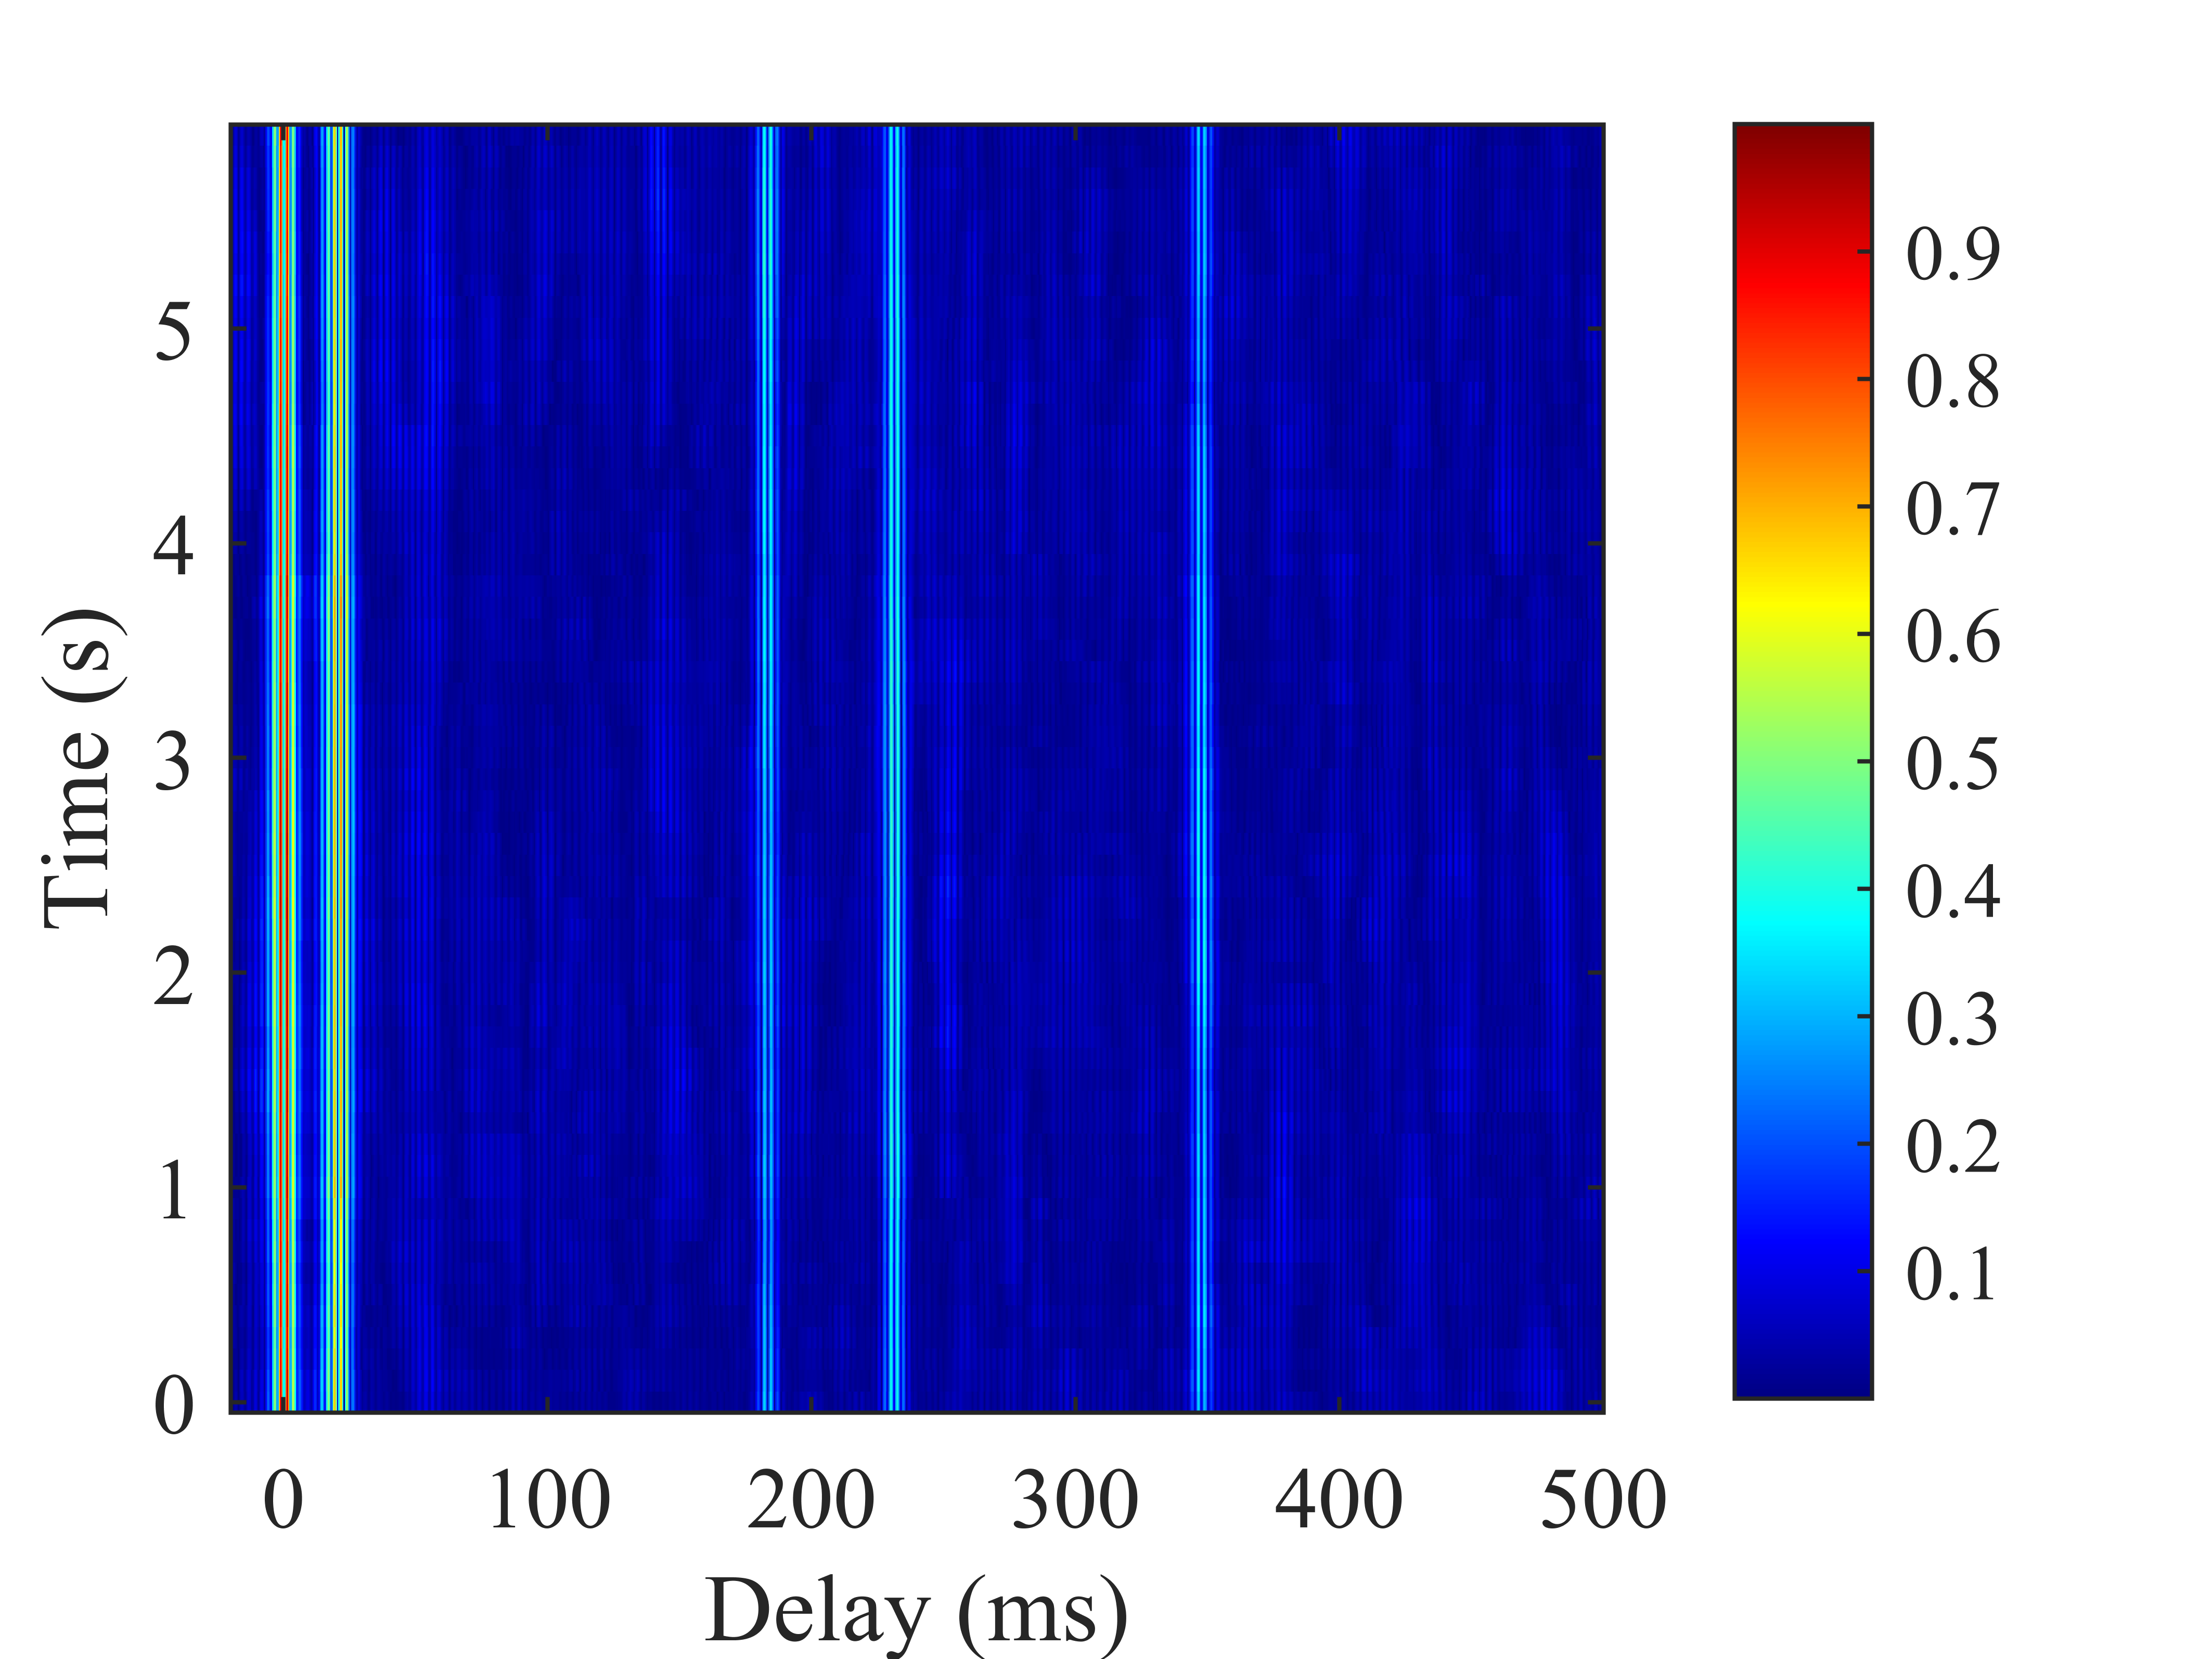
\includegraphics[width=2.5in]{fig/step0.1_window3.png}
\label{parameter_opt_third}}
\hfil
\subfloat[]{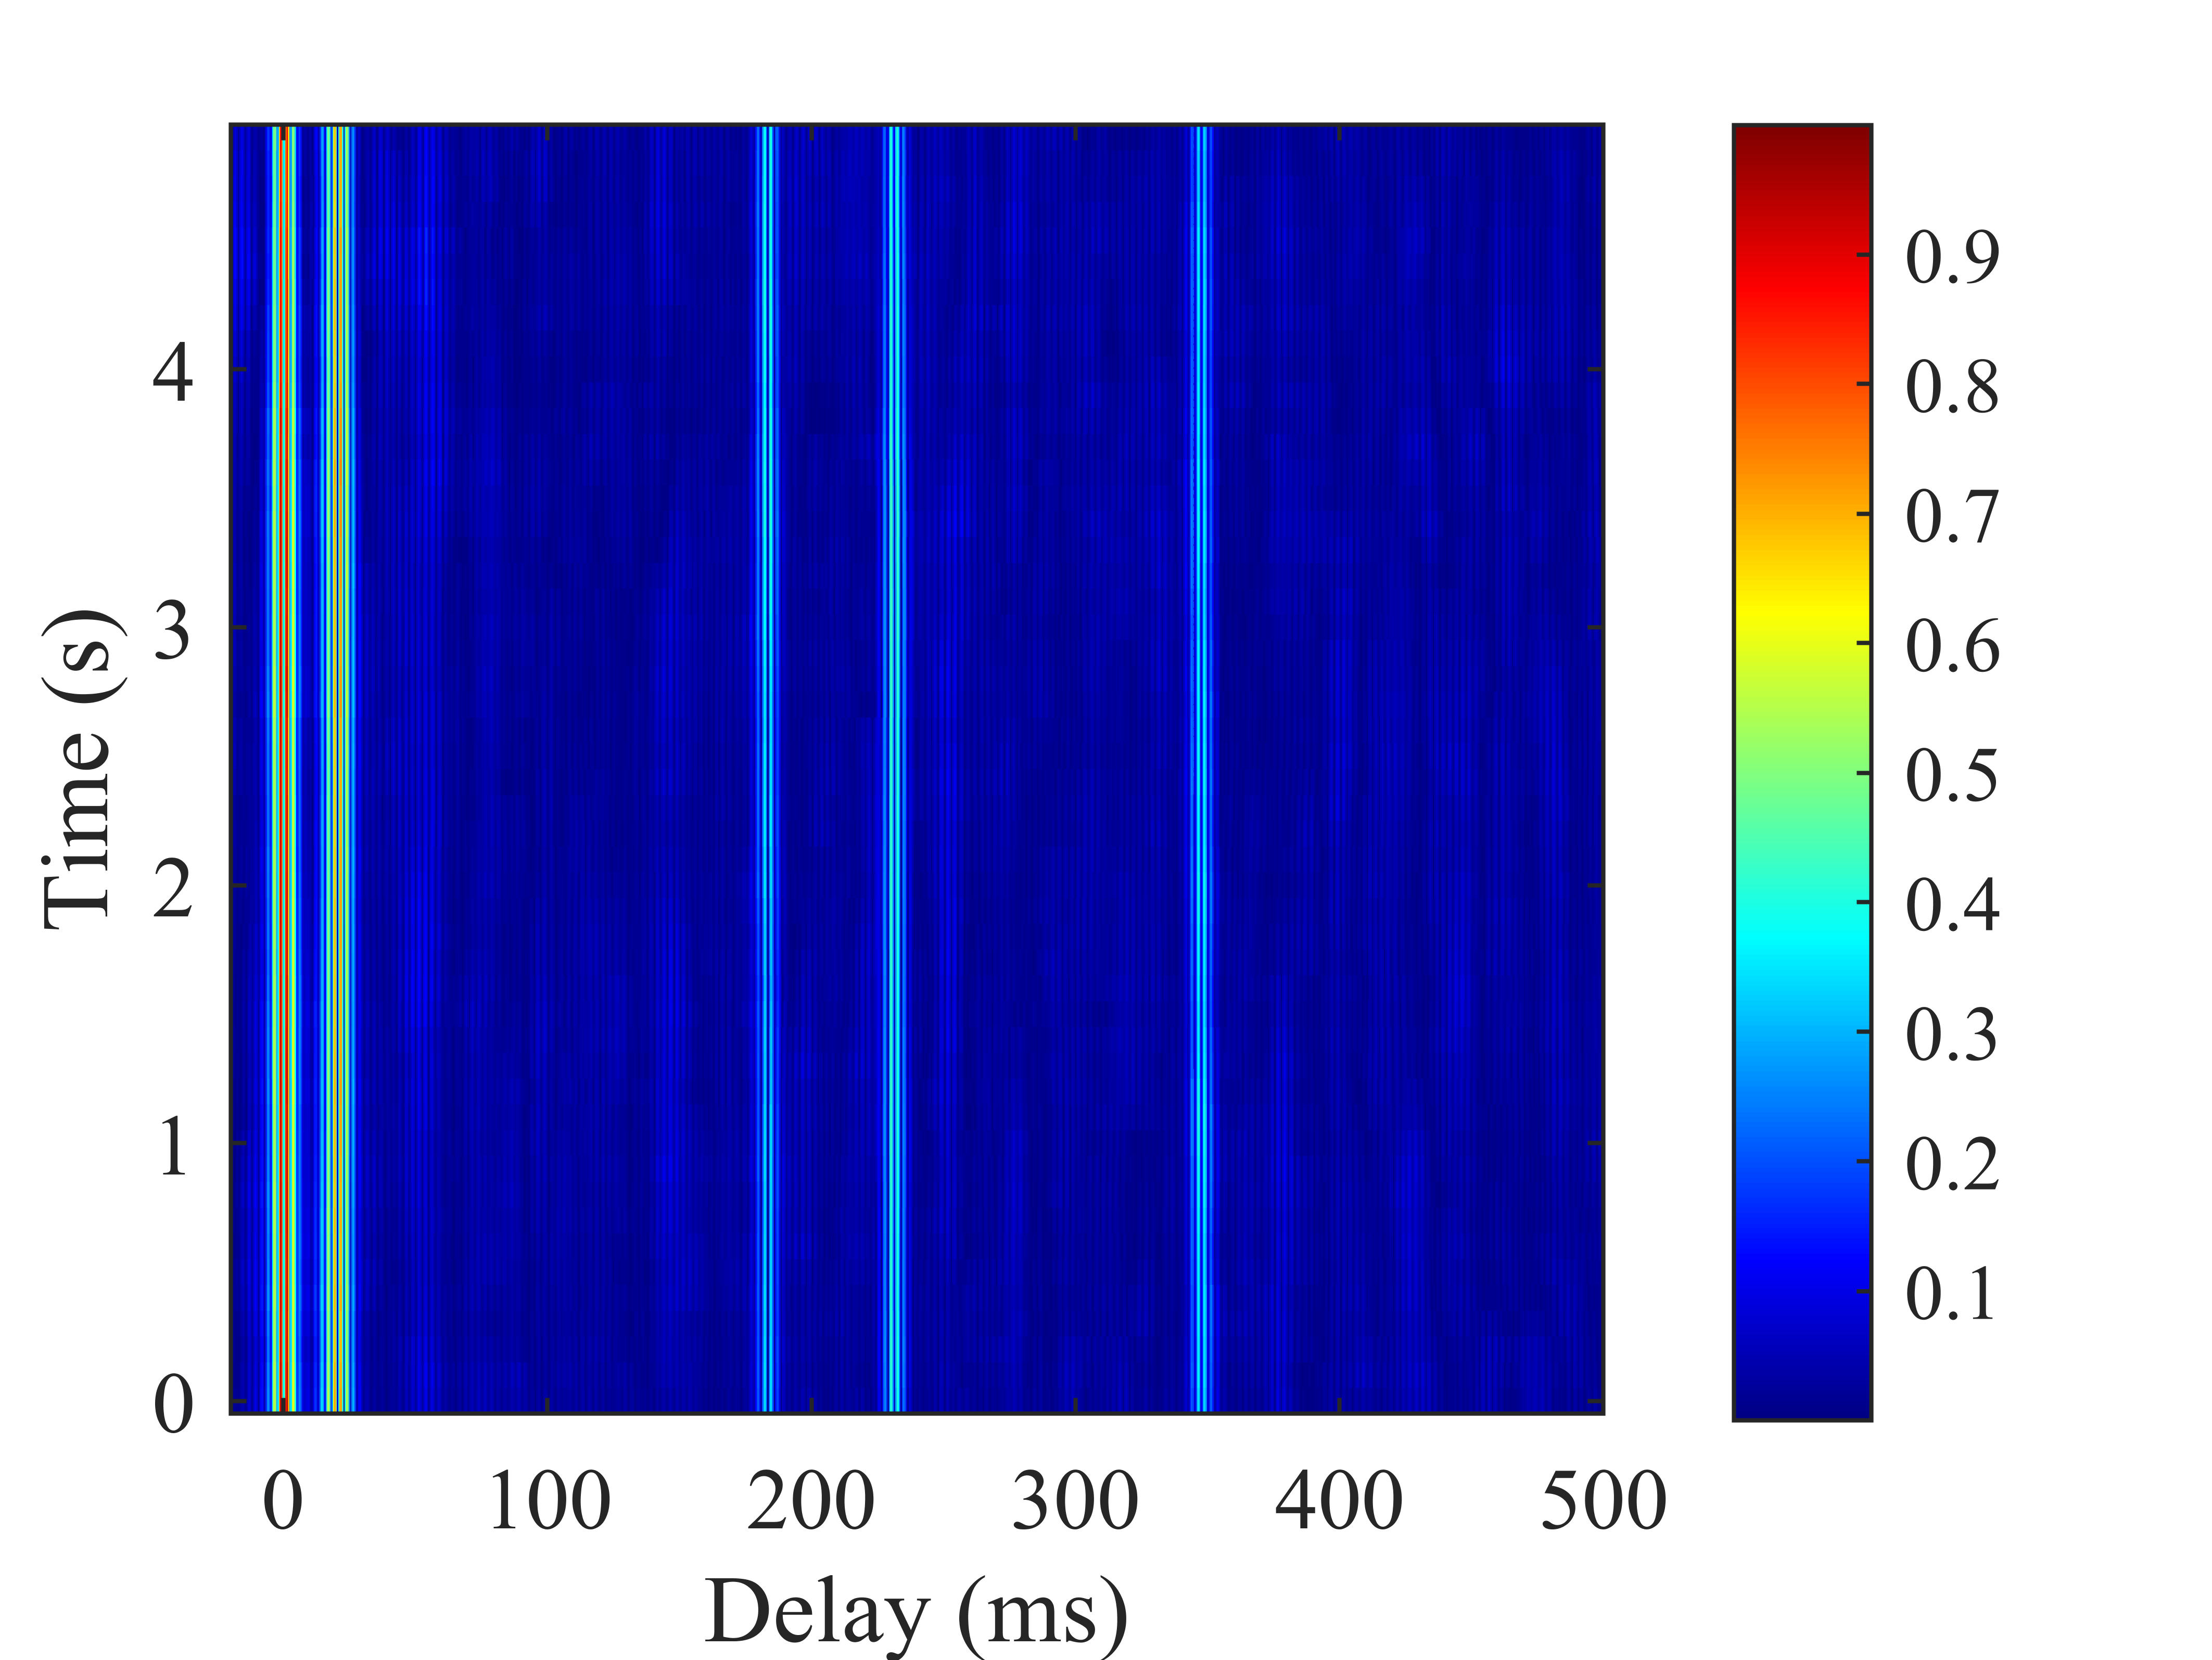
\includegraphics[width=2.5in]{fig/step0.1_window4.png}
\label{parameter_opt_forth}}
\\
\subfloat[]{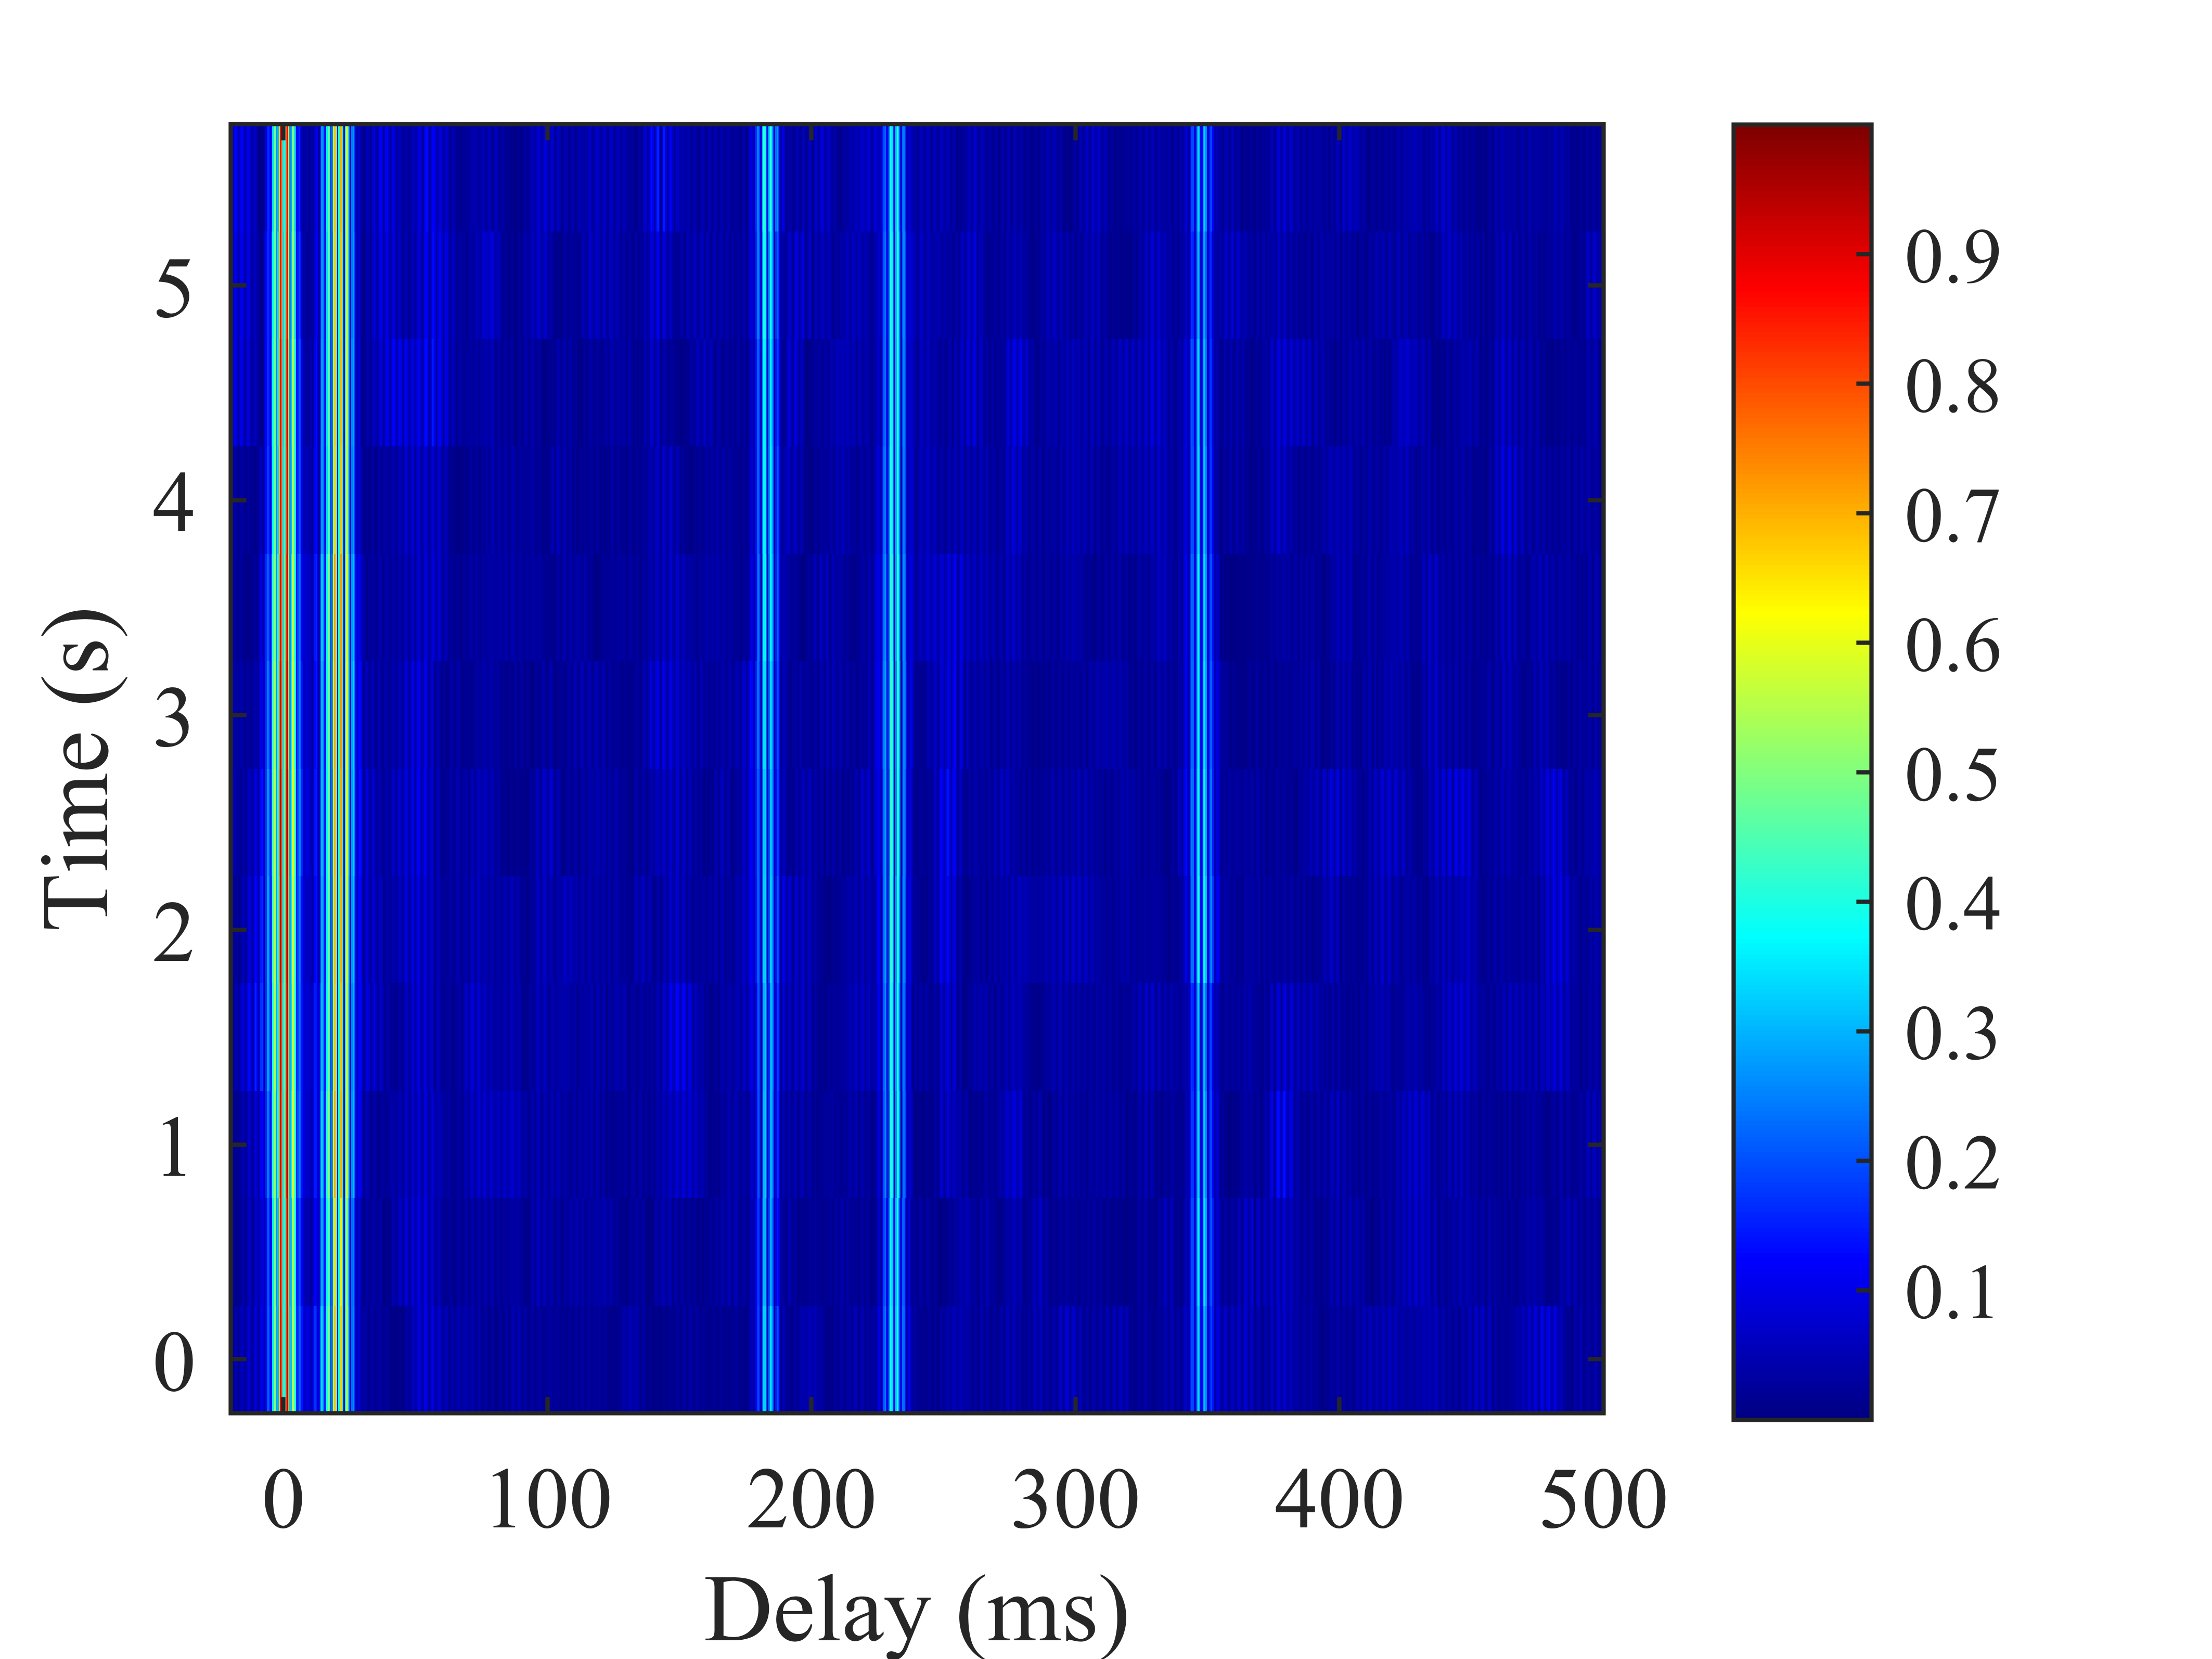
\includegraphics[width=2.5in]{fig/step0.5_window3.png}
\label{parameter_opt_fifth}}
\hfil
\subfloat[]{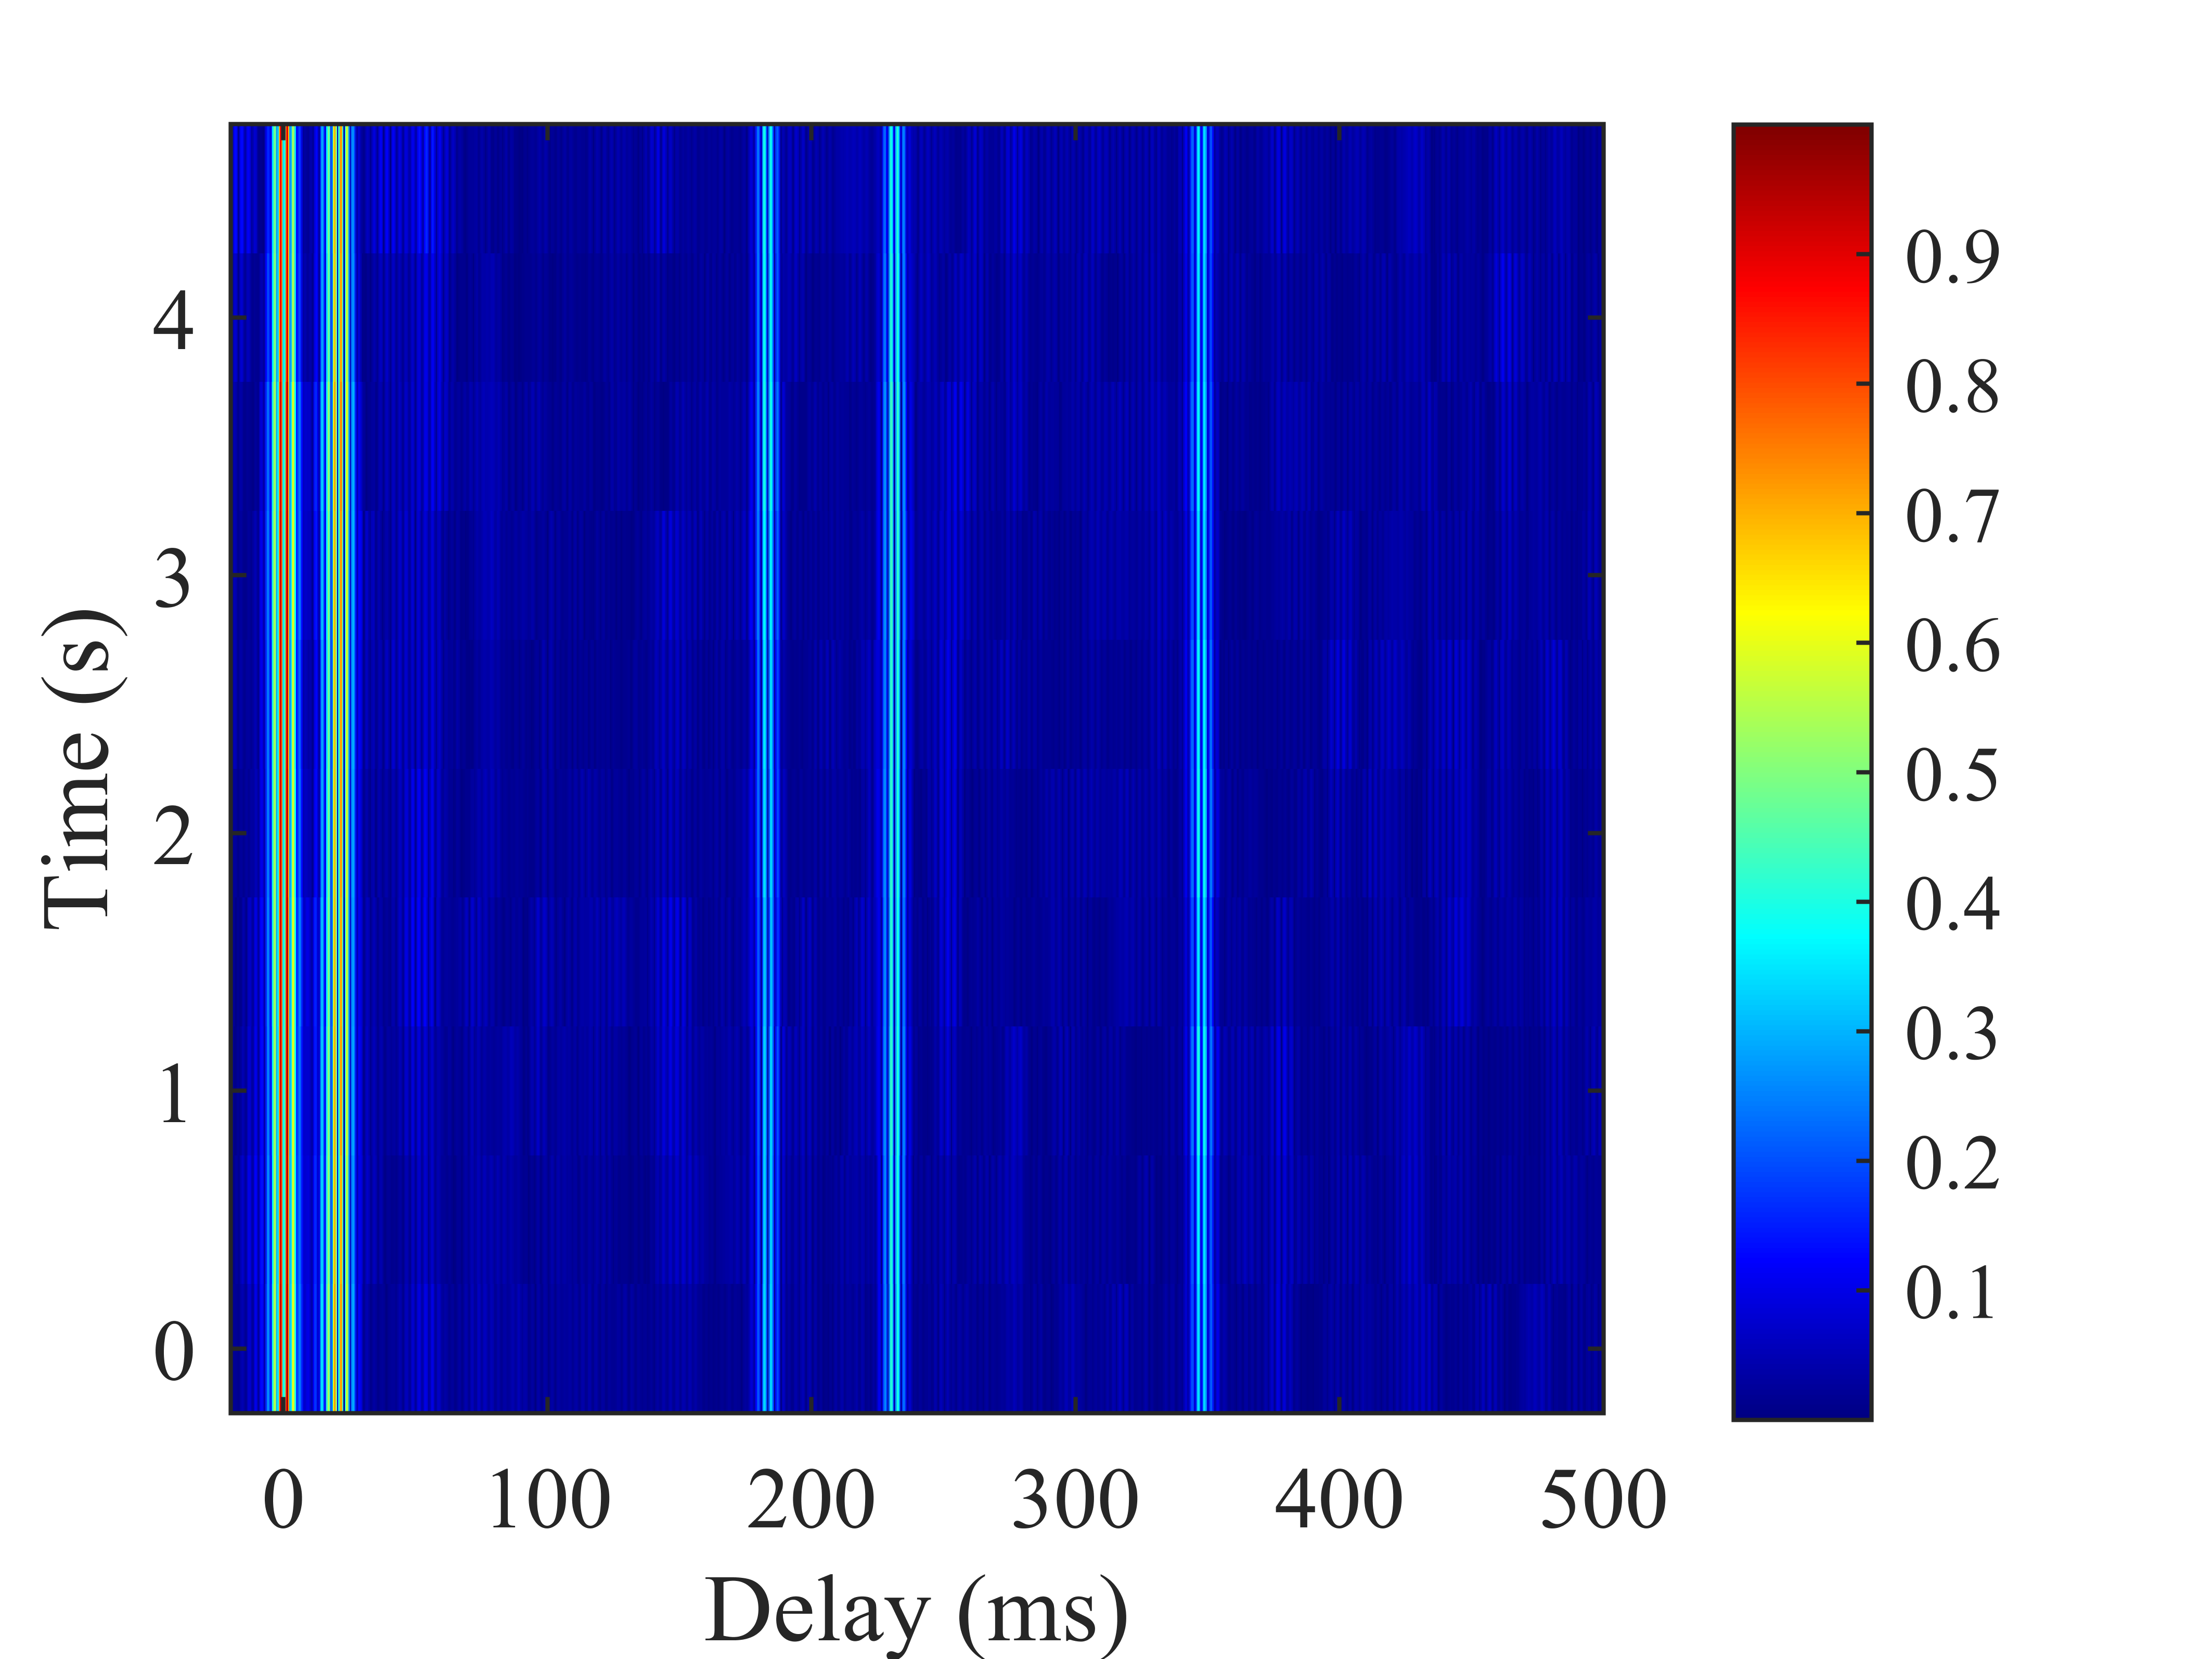
\includegraphics[width=2.5in]{fig/step0.5_window4.png}\label{parameter_opt_sixth}}
\caption{Sliding-window parameter optimization: CIR estimates for varying $(L_w, S)$ combinations: (a) $L_w = 1$, $S = 0.1$; (b) $L_w = 2$, $S = 0.1$; (c) $L_w = 3$, $S = 0.1$; (d) $L_w = 4$, $S = 0.1$; (e) $L_w = 3$, $S = 0.5$; (f) $L_w = 4$, $S = 0.5$.}
\label{fig:parameter_opt}
\end{figure*}

Accordingly, we adopted $L_w = 3$~s and $S = 0.1$~s for experimental-data processing, achieving an effective temporal resolution of 0.1~s with a 30-fold overlap. The complete estimation workflow is summarized in Fig.~\ref{fig:flowchart}.

\begin{figure*}[!t]
\centering
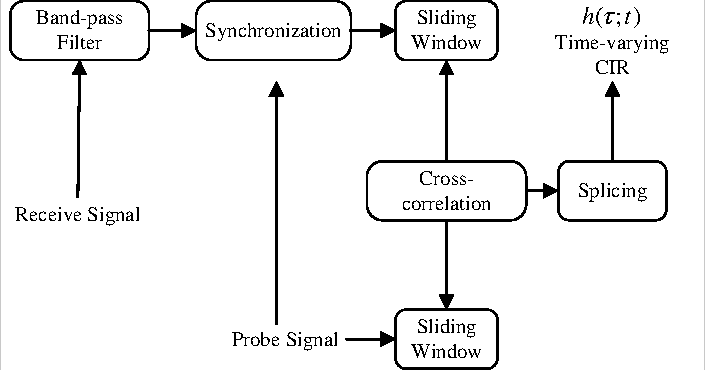
\includegraphics[width=0.62\textwidth]{fig/Flowchart.pdf}
\caption{Flowchart of sliding-window-based time-varying CIR estimation.}
\label{fig:flowchart}
\end{figure*}

\subsection{Channel Characterization Metrics}

From the estimated time-varying CIRs $\mathbf{H}$, we derive the following second-order statistics for comprehensive channel characterization\cite{ref18}.

\textbf{Delay-domain metrics:} The delay power spectrum $P_d(\tau)$ is obtained by averaging $|\hat{\mathbf{h}}_k[\tau]|^2$ over observation time. From this, the mean excess delay and RMS delay spread are computed as:
\begin{equation}
\tau_m = \frac{\int \tau P_d(\tau) \, d\tau}{\int P_d(\tau) \, d\tau}, \quad
\tau_{\mathrm{rms}} = \sqrt{\frac{\int (\tau - \tau_m)^2 P_d(\tau) \, d\tau}{\int P_d(\tau) \, d\tau}}
\end{equation}

\textbf{Time-domain metrics:} The time-correlation function $R_t(\Delta t)$ quantifies channel decorrelation over time intervals. The coherence time $T_c(\rho)$ is defined as the time lag where $|R_t(\Delta t)|$ falls below threshold $\rho$ (typically 0.5 or 0.9).

\textbf{Frequency-domain metrics:} The frequency-correlation function $R_f(\Delta f)$ yields the coherence bandwidth $B_c(\rho)$, analogously defined as the frequency separation where correlation drops below $\rho$.

\textbf{Doppler-domain metrics:} The scattering function $S_c(\tau, \nu)$, obtained via Fourier transform of $R_t(\Delta t)$, characterizes the Doppler spectrum. The RMS Doppler spread is:
\begin{equation}
\nu_{\mathrm{rms}} = \sqrt{\frac{\int (\nu - \nu_m)^2 S_c(\nu) \, d\nu}{\int S_c(\nu) \, d\nu}}
\end{equation}
where $\nu_m$ is the mean Doppler shift.

These metrics form the basis of the depth-dependent analysis presented in Section~\ref{sec:results} and the system-design implications discussed in Section~\ref{sec:mechanism}.


\section{Impact of AUV Vertical Mobility on Channel Dynamics}
\label{sec:results}

This section presents the core experimental findings on how deep sea acoustic channel characteristics evolve with receiver depth. We first examine multipath evolution using time-varying CIRs and power delay profiles (PDPs), then quantify depth-dependent statistical parameters, and finally demonstrate the breakdown of classical channel relationships in this environment.

\subsection{Evolution of Multipath Structure with Depth}
\label{subsec:multipath}

The multipath structure varies markedly across the vertical array, transitioning from relatively simple to highly complex and then back to sparse as the depth increases. This non-monotonic evolution is a key finding of this study.

Fig.~\ref{fig:cir_time} shows time-varying CIR magnitudes at the four measurement depths over a 10-s observation window. At 475.8~m, the shallowest receiver position in the main thermocline, the CIR is comparatively simple: acoustic energy is concentrated primarily in two arrivals, namely the direct path and a robust surface reflection, exhibiting minimal inter-path delay and relatively stable amplitudes.

At 624.8~m, the mid-thermocline, the channel becomes more intricate. Although the direct path remains dominant, energy spreads over multiple closely spaced arrivals. A weak but clear component appears near 140~ms, suggesting activation of longer refracted or bottom-interacting paths. Relative to the 475.8~m case, the strongest reflected path is attenuated, consistent with increased geometric spreading and boundary loss at steeper ray angles.

The most pronounced transformation appears at 824.8~m, the lower main thermocline. The CIR exhibits a dense multipath pattern with arrivals distributed over approximately 400~ms. Notably, an energy inversion is observed, where the third arrival exceeds the second in power. This ordering is inconsistent with simple geometric expectations and strongly suggests caustic focusing\cite{ref19}, i.e., localized intensity enhancement due to ray convergence near the sound-channel axis. This depth therefore represents the peak multipath complexity observed in the experiment.

In the main thermocline base (924.8~m), near the seabed, the channel becomes sparser again. Despite the larger traversed water column, the number of resolvable components decreases. This behavior is consistent with enhanced bottom absorption and scattering suppressing long, grazing paths that contributed to the dense structure at 824.8~m.

Fig.~\ref{fig:pdp} confirms these trends in the time-averaged PDPs. The 475.8~m profile shows two sharp dominant peaks; the 624.8~m profile broadens with additional weaker lobes; the 824.8~m profile exhibits the most diffuse, cluster-like distribution; and the 924.8~m profile returns to a more concentrated but asymmetric shape with delayed yet weaker secondary arrivals. This non-monotonic multipath evolution directly dictates the required baseband computational resources. The dense and elongated multipath clustering observed at 824.8 m necessitates a significantly expanded equalizer memory to mitigate severe ISI. For power-constrained AUVs, this expansion translates to a substantial increase in computational burden and energy drain compared to operating in the sparser multipath regimes at 475.8 m or 924.8 m. 

\begin{figure*}[!t]
\centering
\subfloat[]{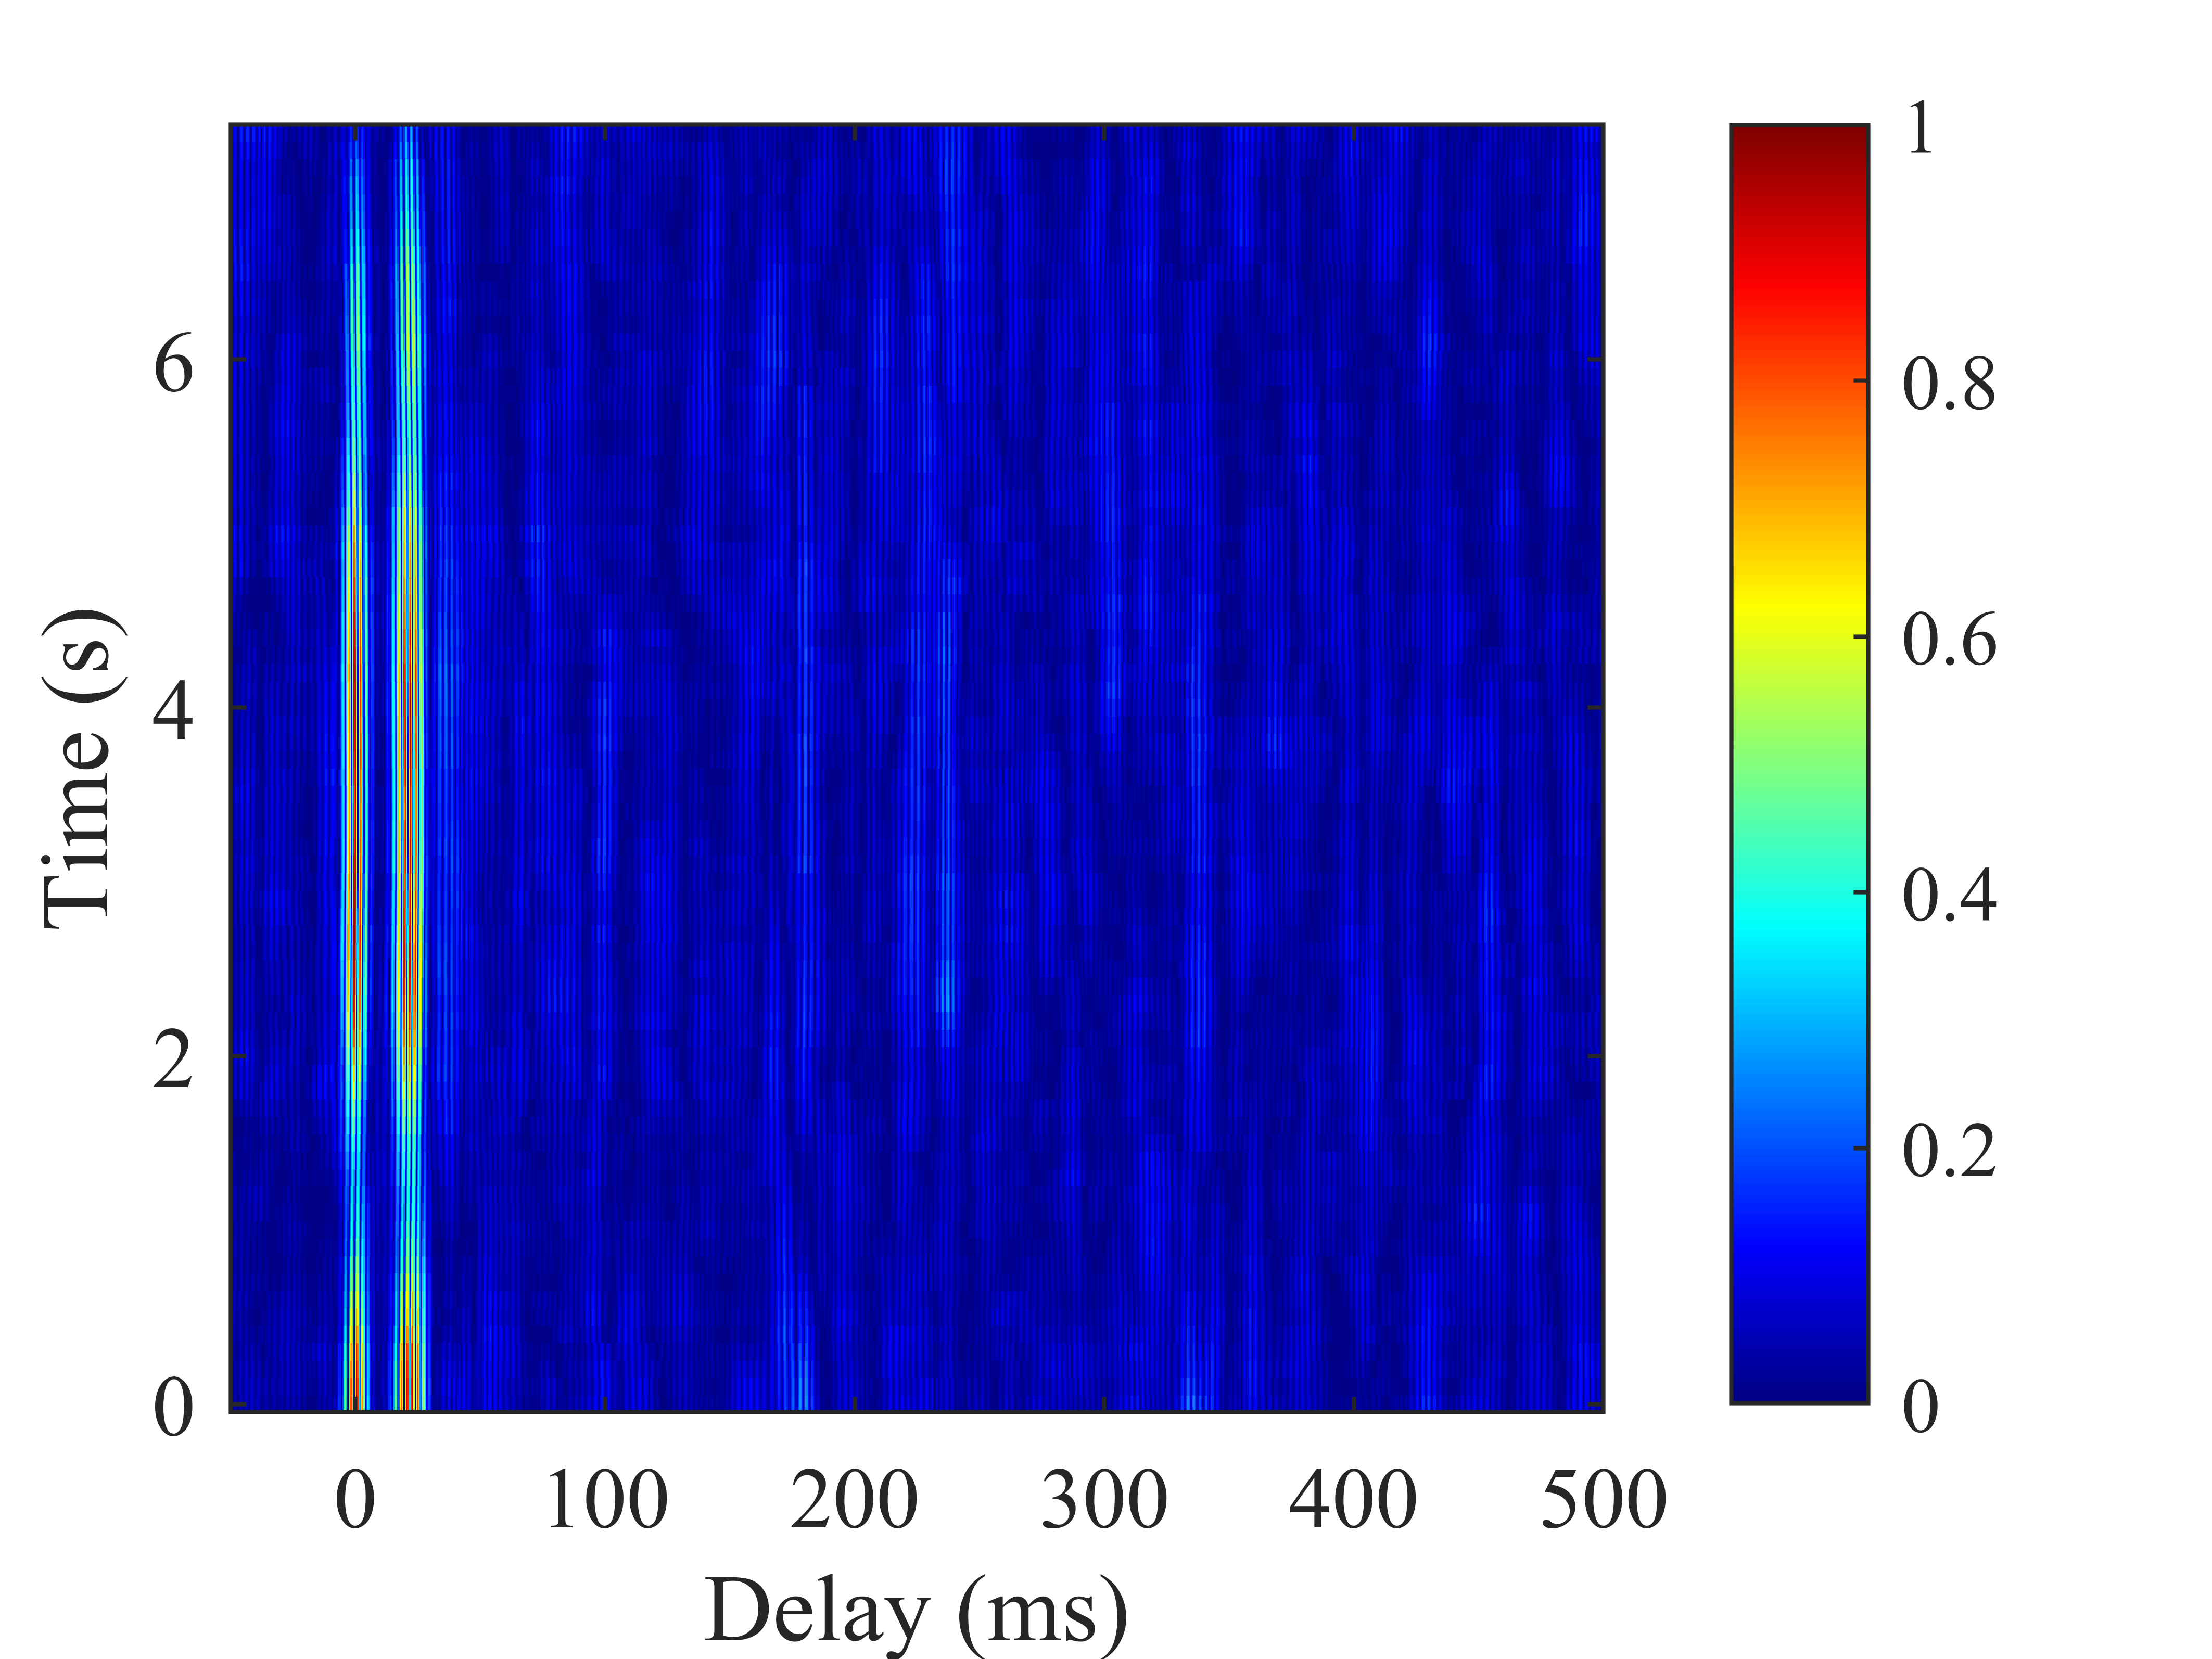
\includegraphics[width=2.5in]{fig/CIR(a).png}
\label{cir_time_first}}
\hfil
\subfloat[]{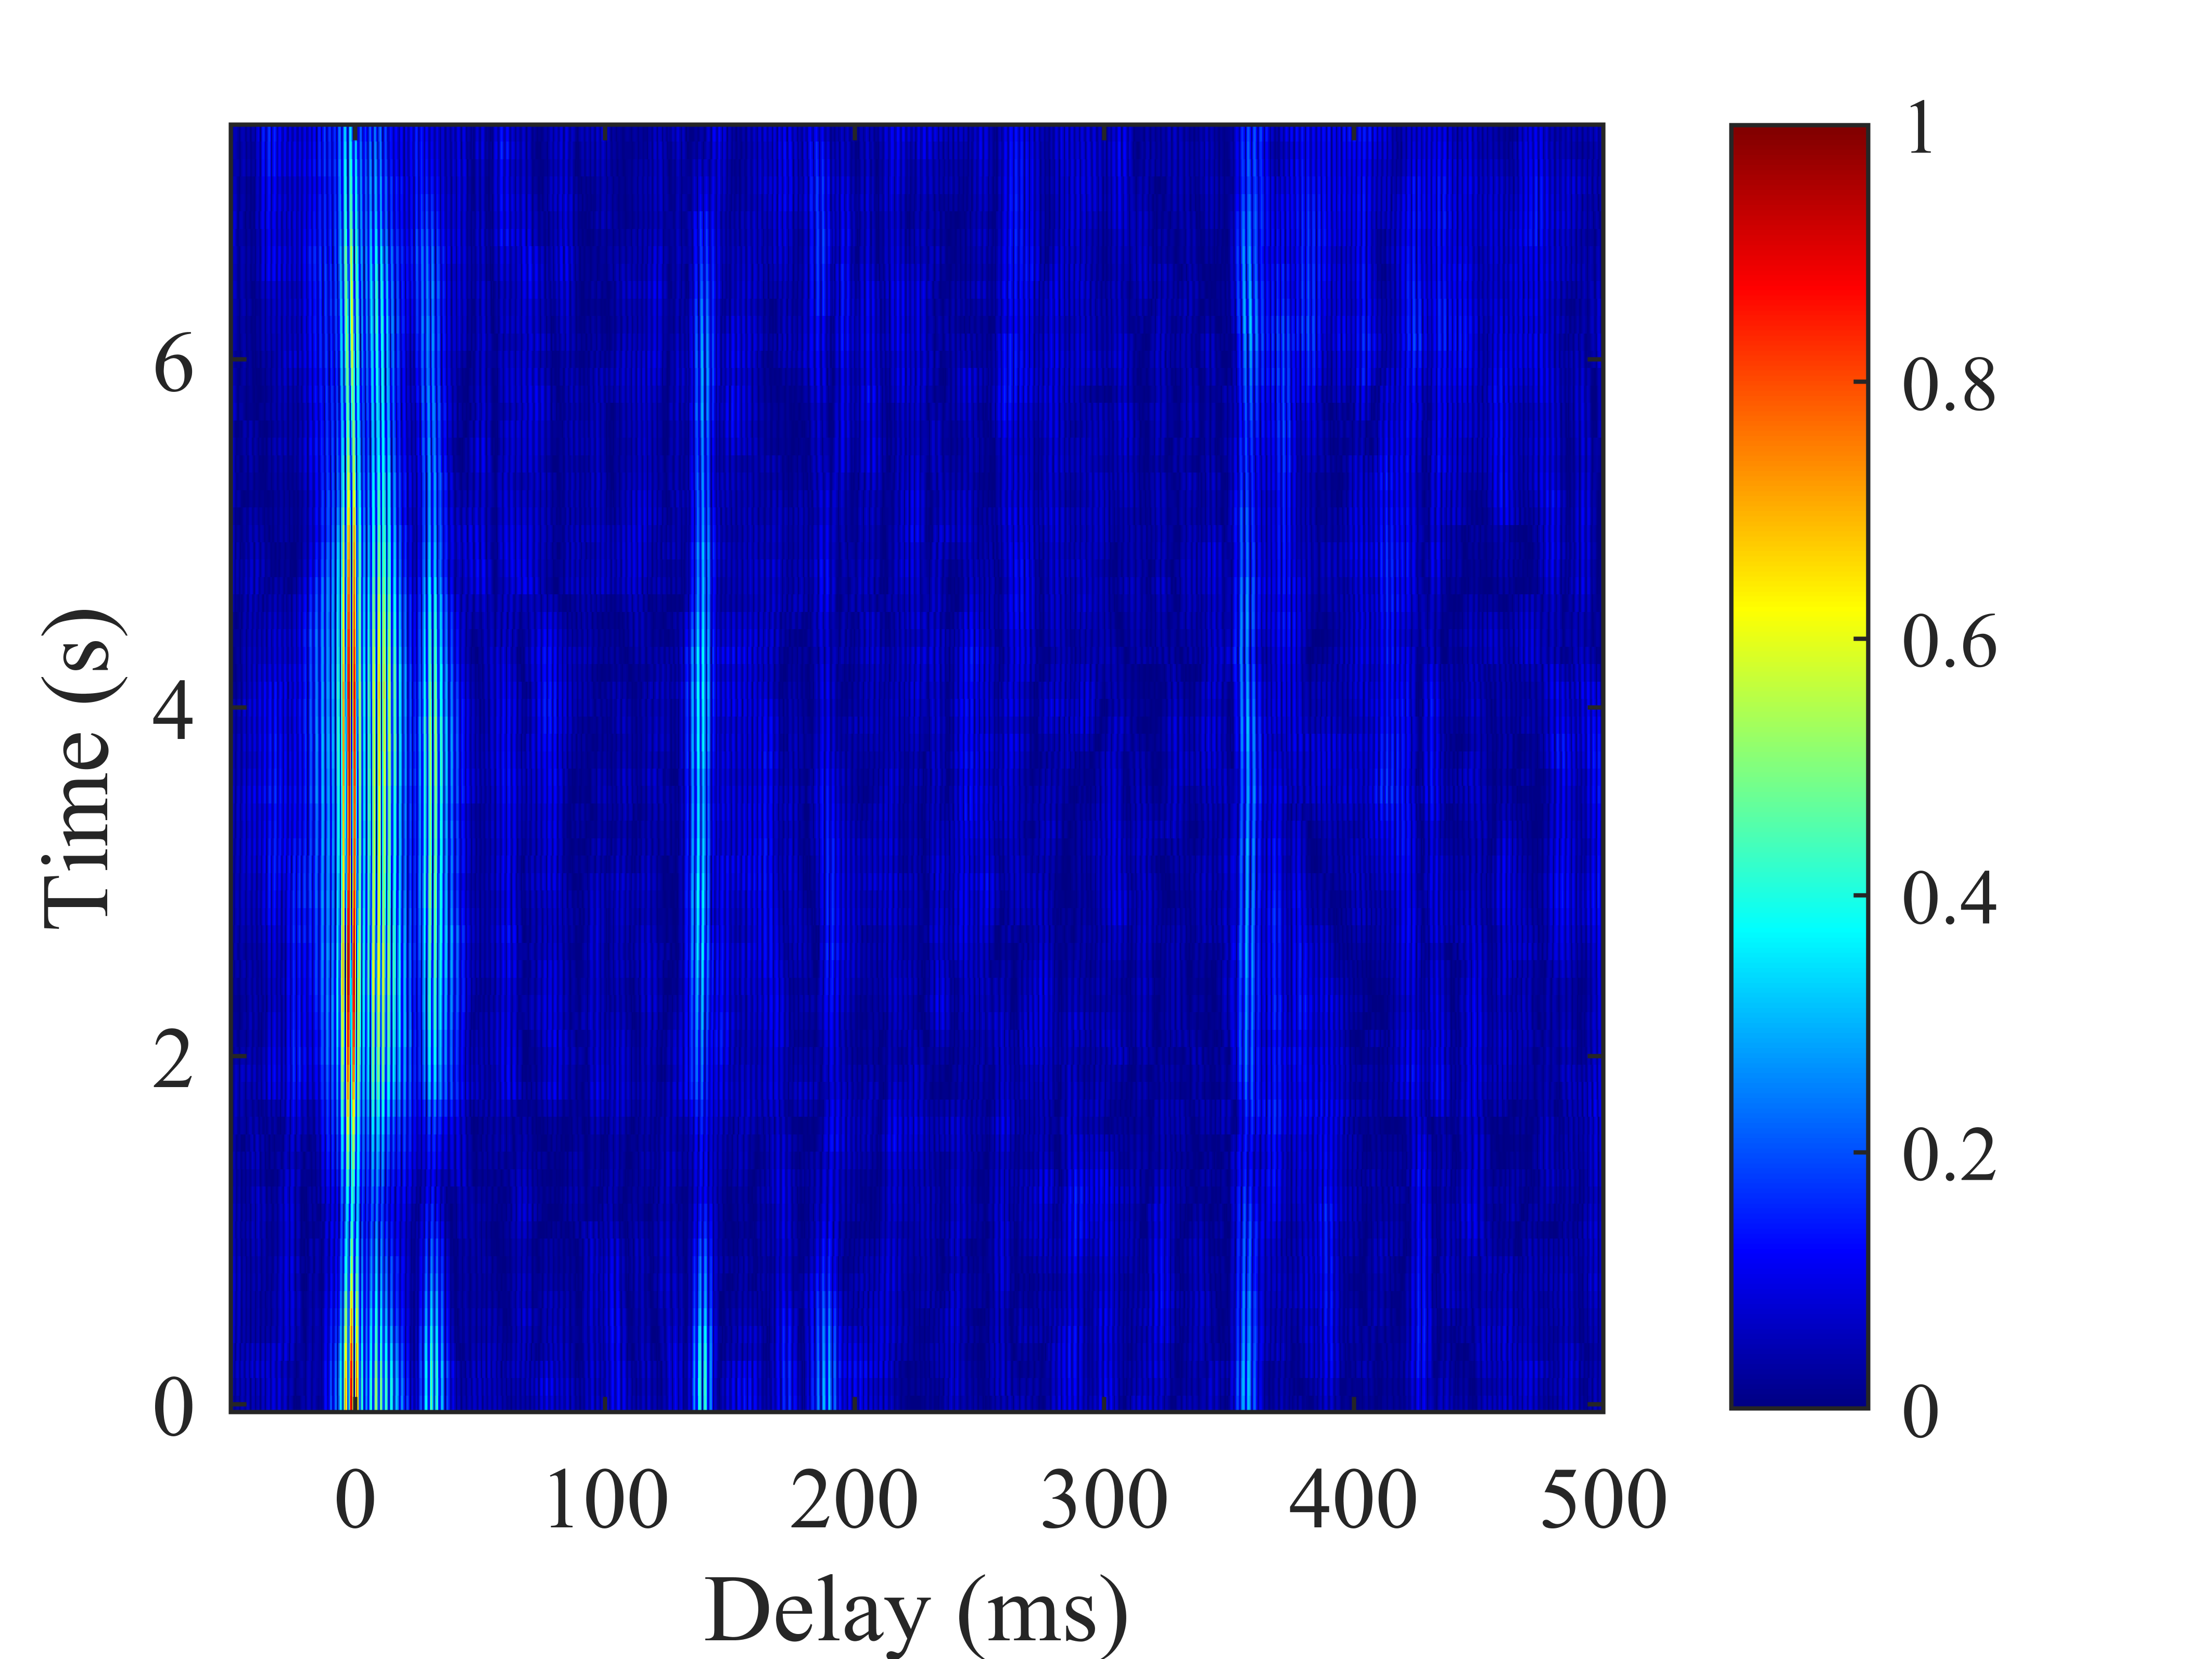
\includegraphics[width=2.5in]{fig/CIR(b).png}
\label{cir_time_second}}
\\
\subfloat[]{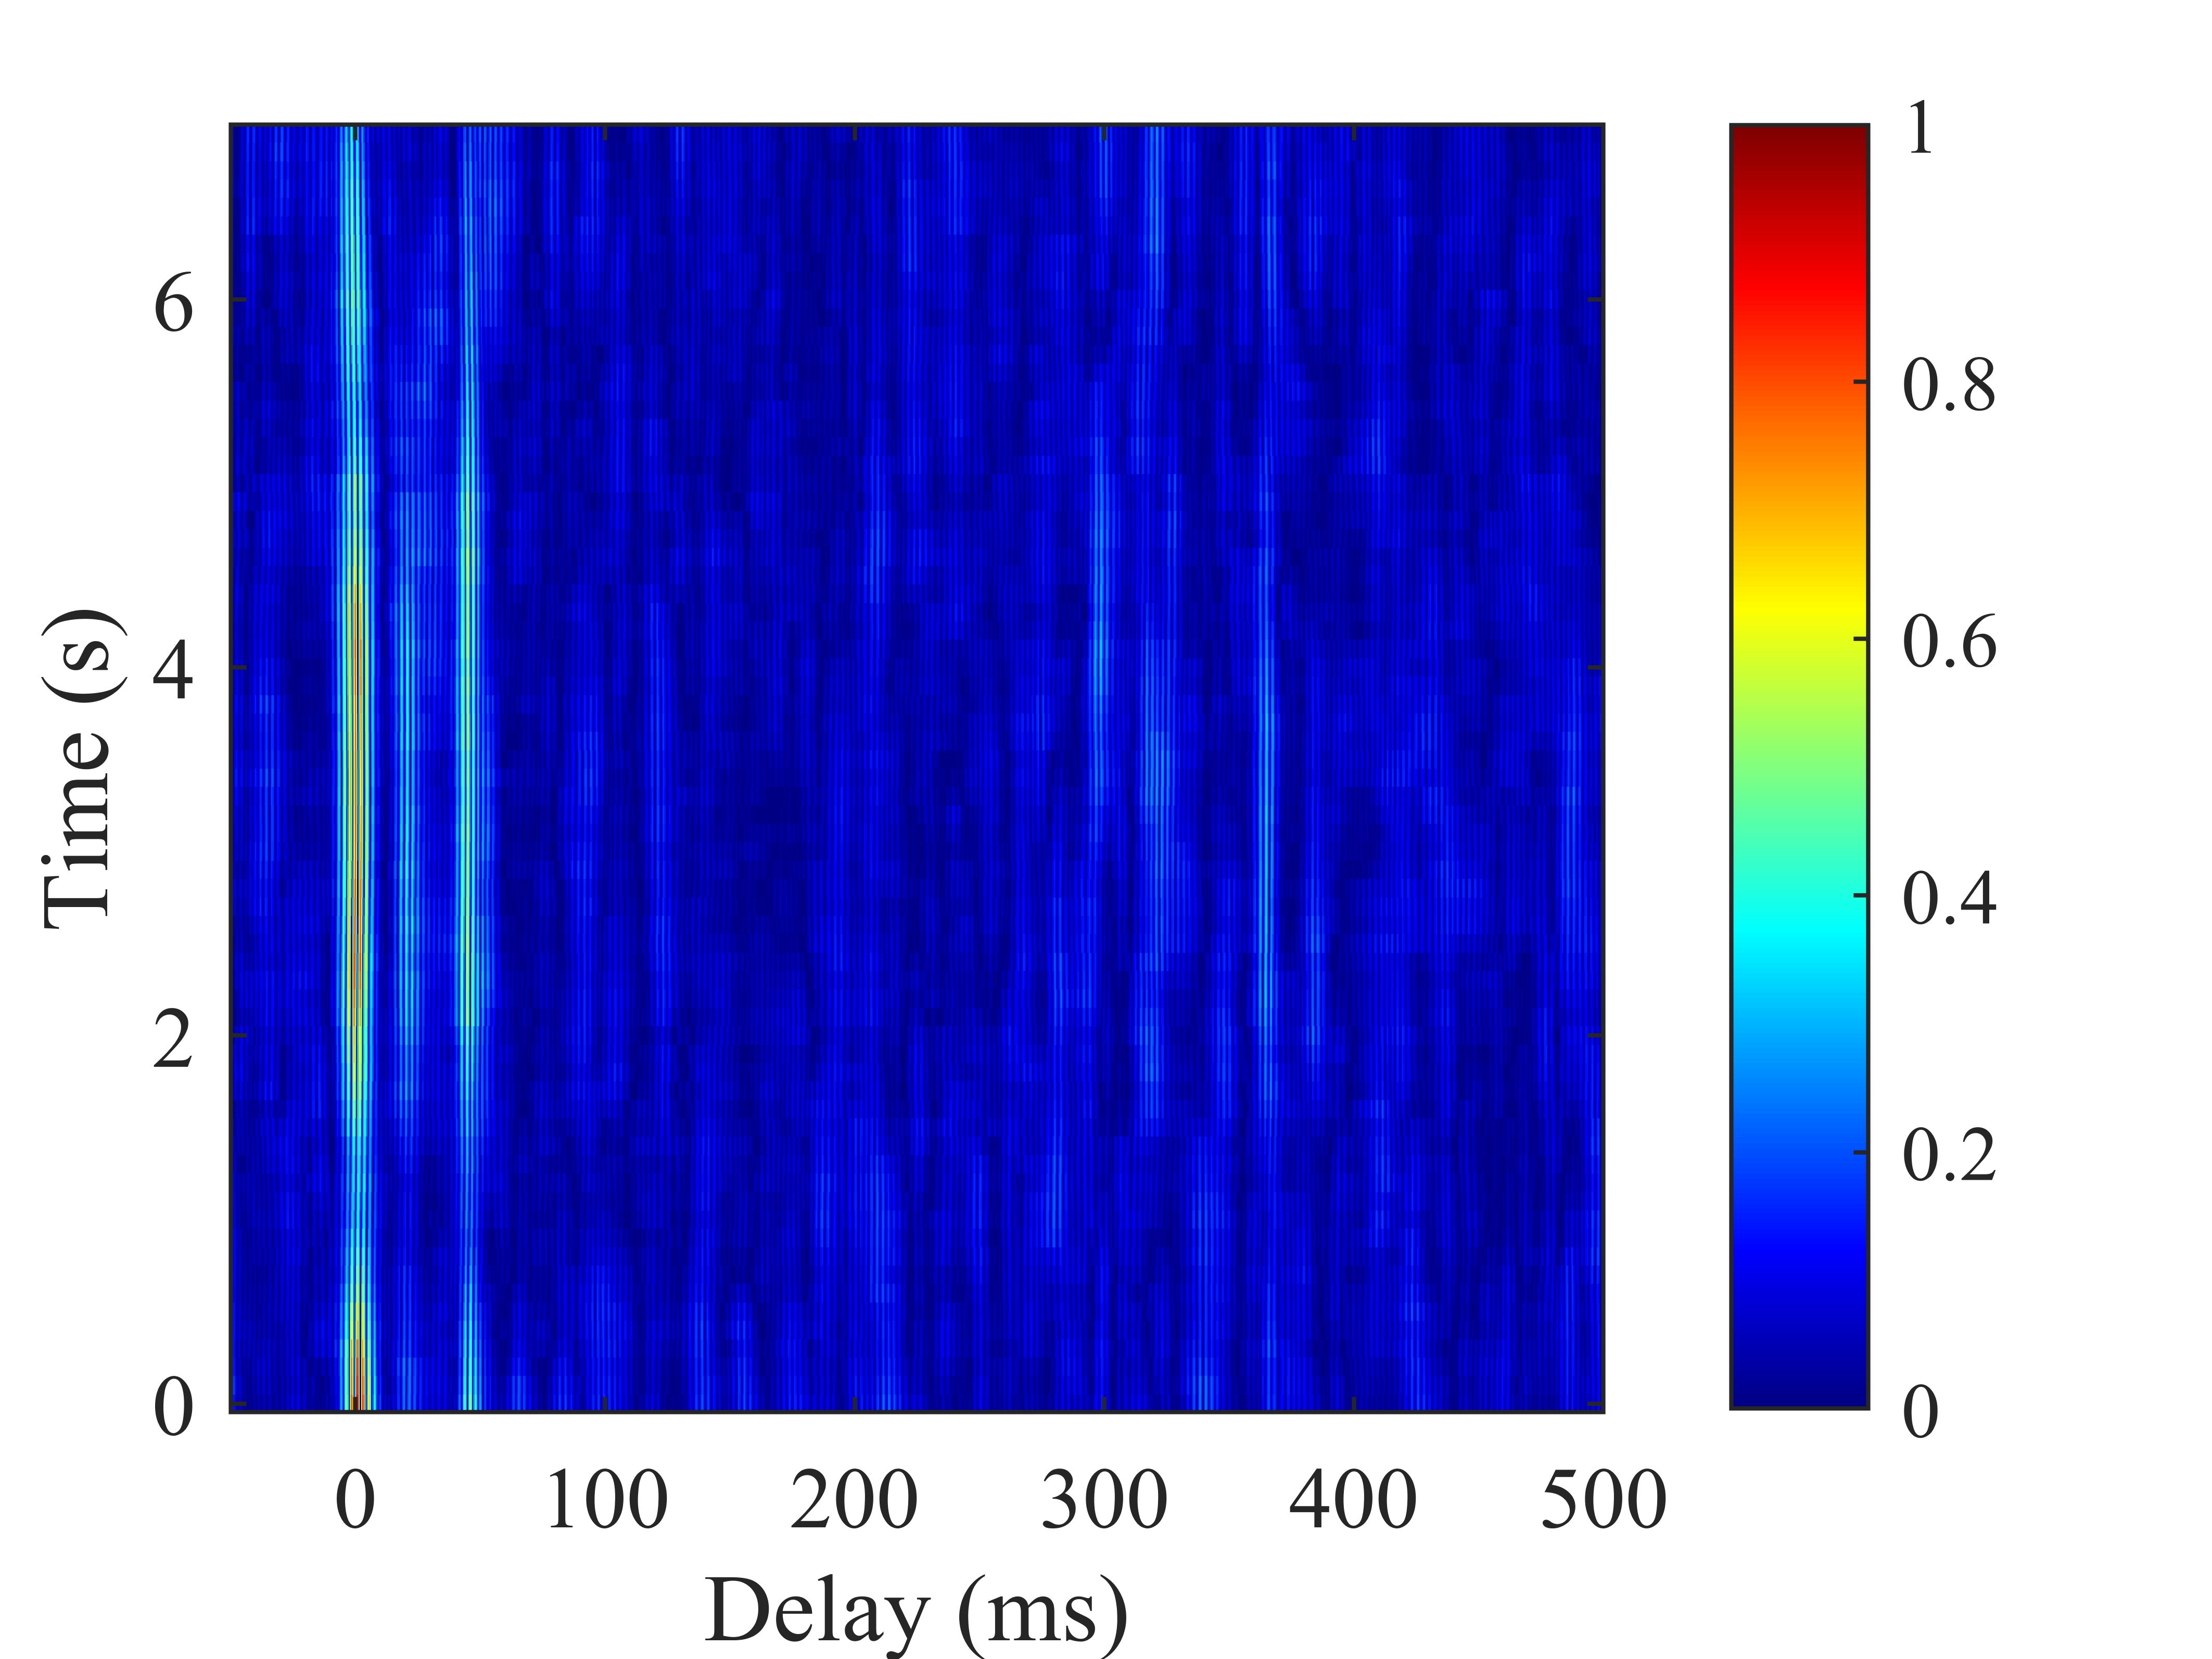
\includegraphics[width=2.5in]{fig/CIR(c).png}
\label{cir_time_third}}
\hfil
\subfloat[]{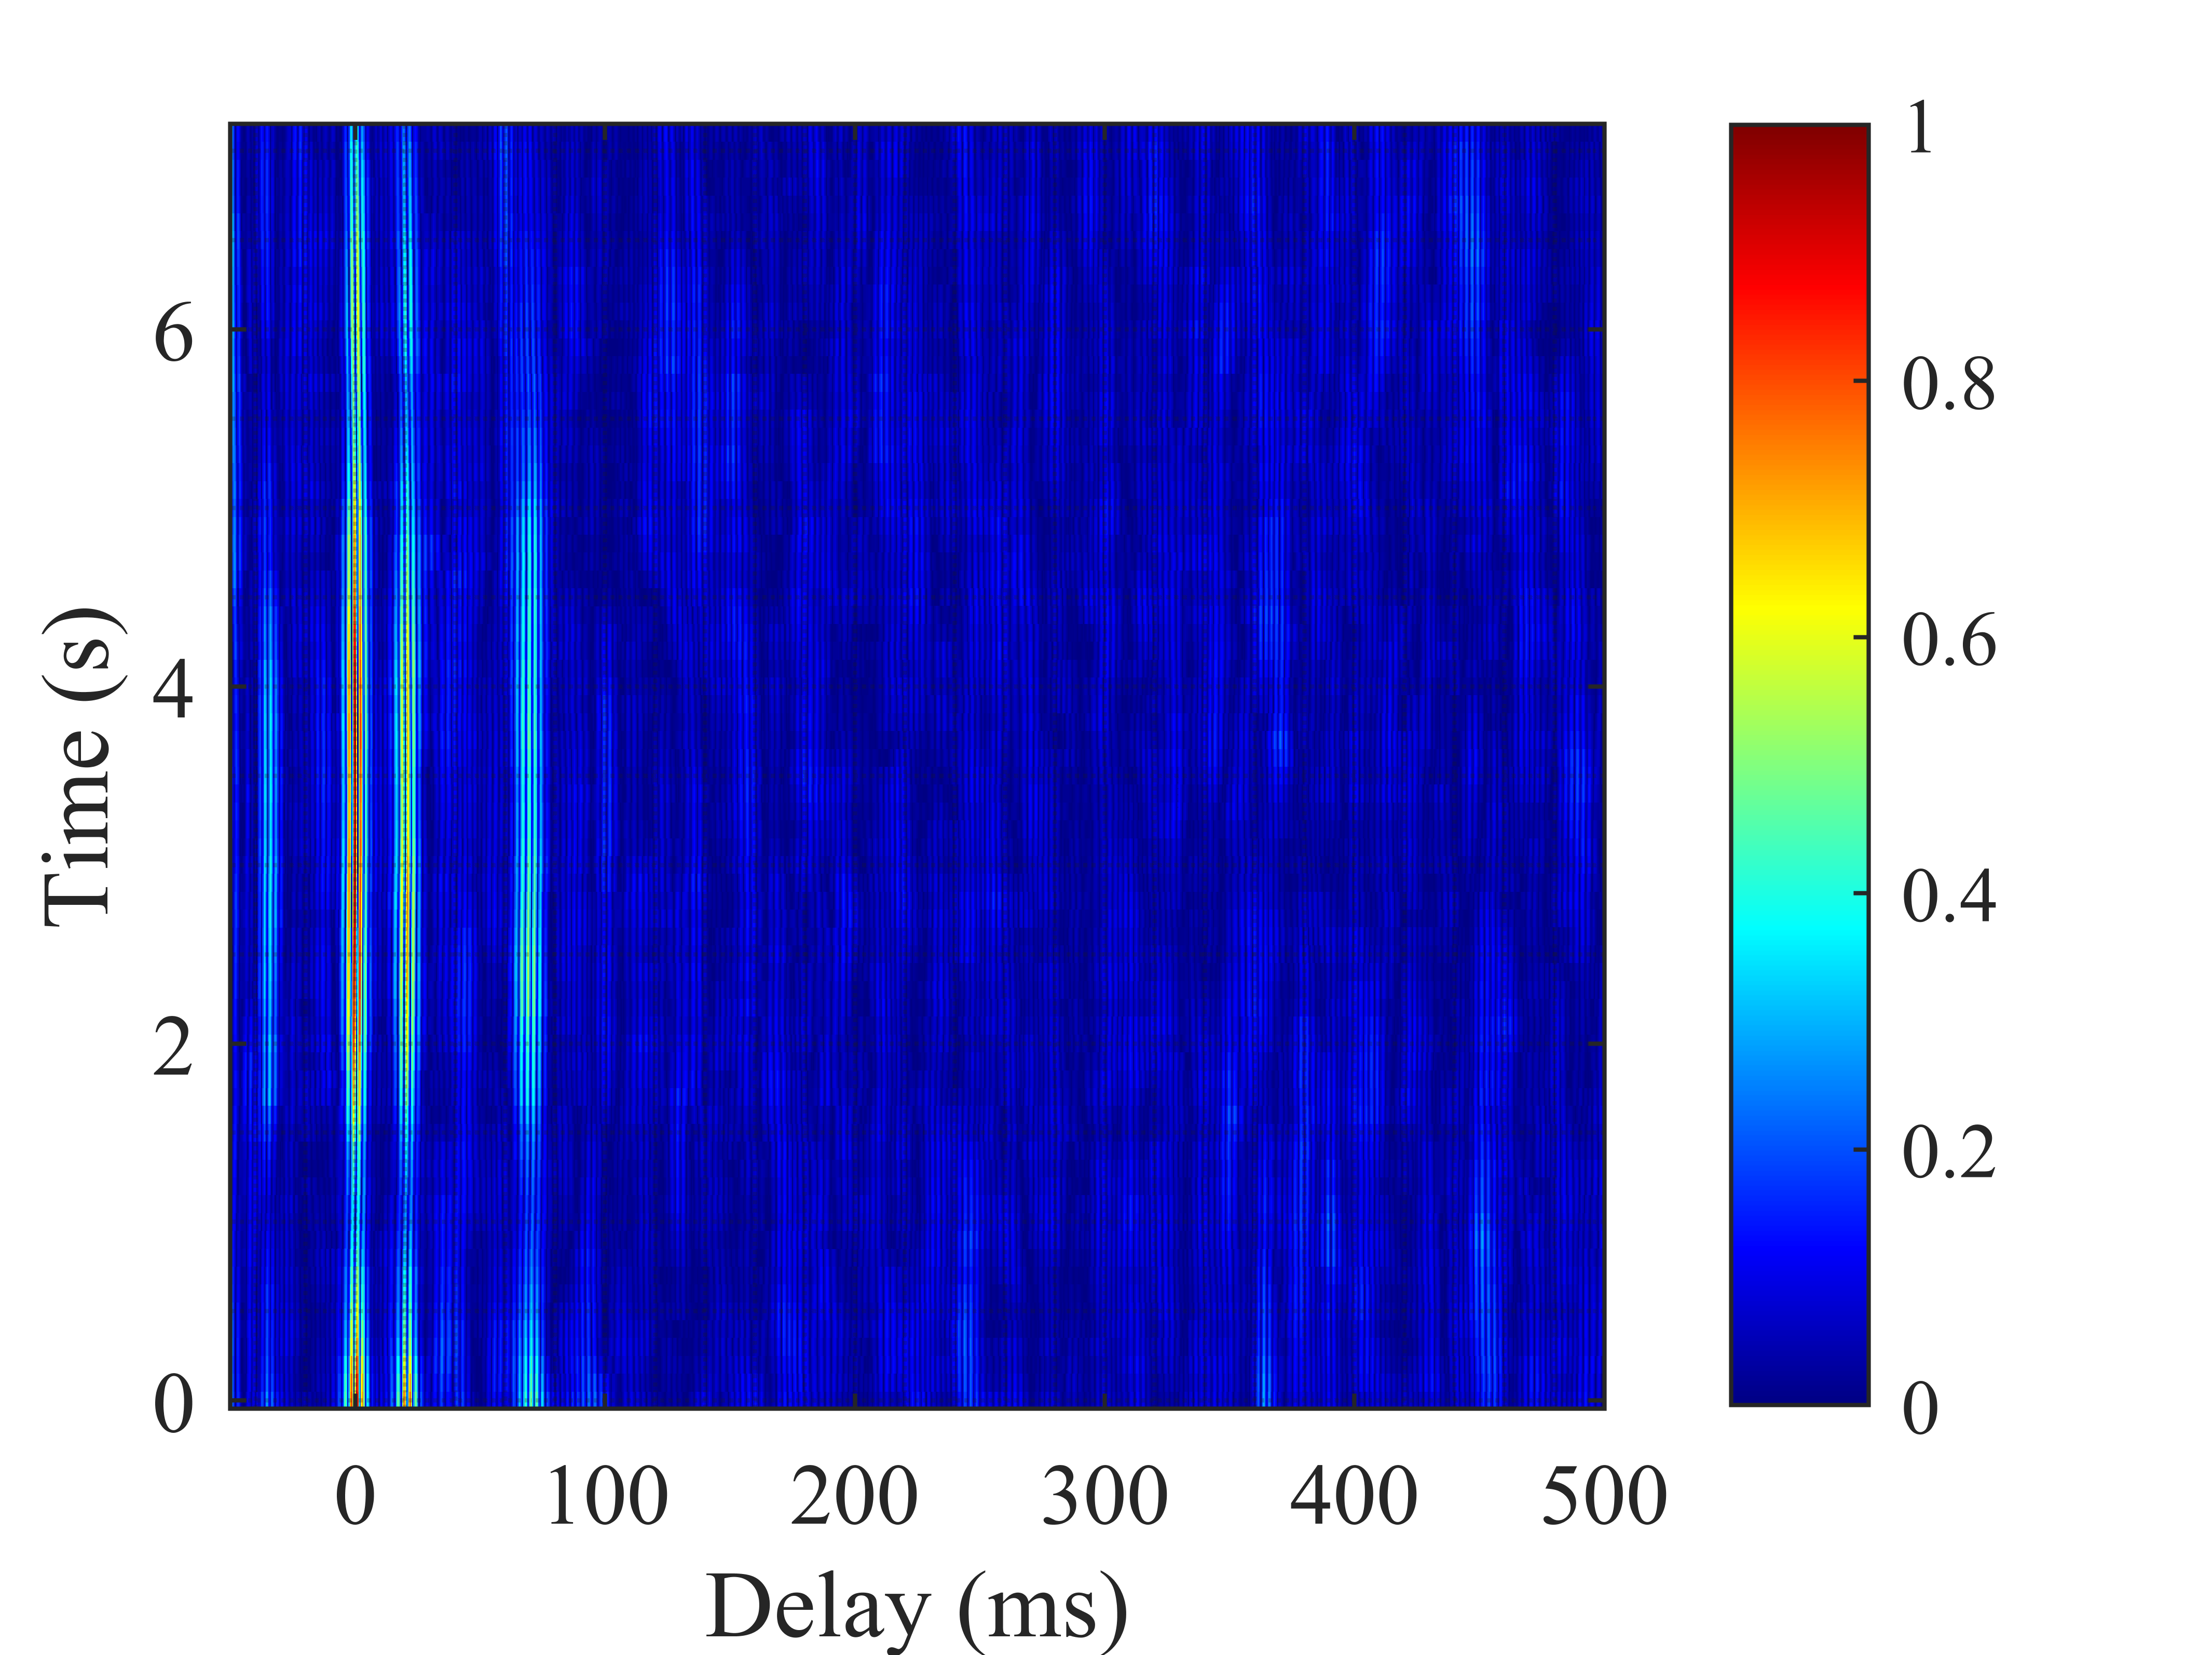
\includegraphics[width=2.5in]{fig/CIR(d).png}
\label{cir_time_forth}}
\caption{Time-varying CIR magnitude at four receiver depths over a 10-s observation period: (a) 475.8~m, (b) 624.8~m, (c) 824.8~m, (d) 924.8~m.}
\label{fig:cir_time}
\end{figure*}

\begin{figure}[!t]
\centering
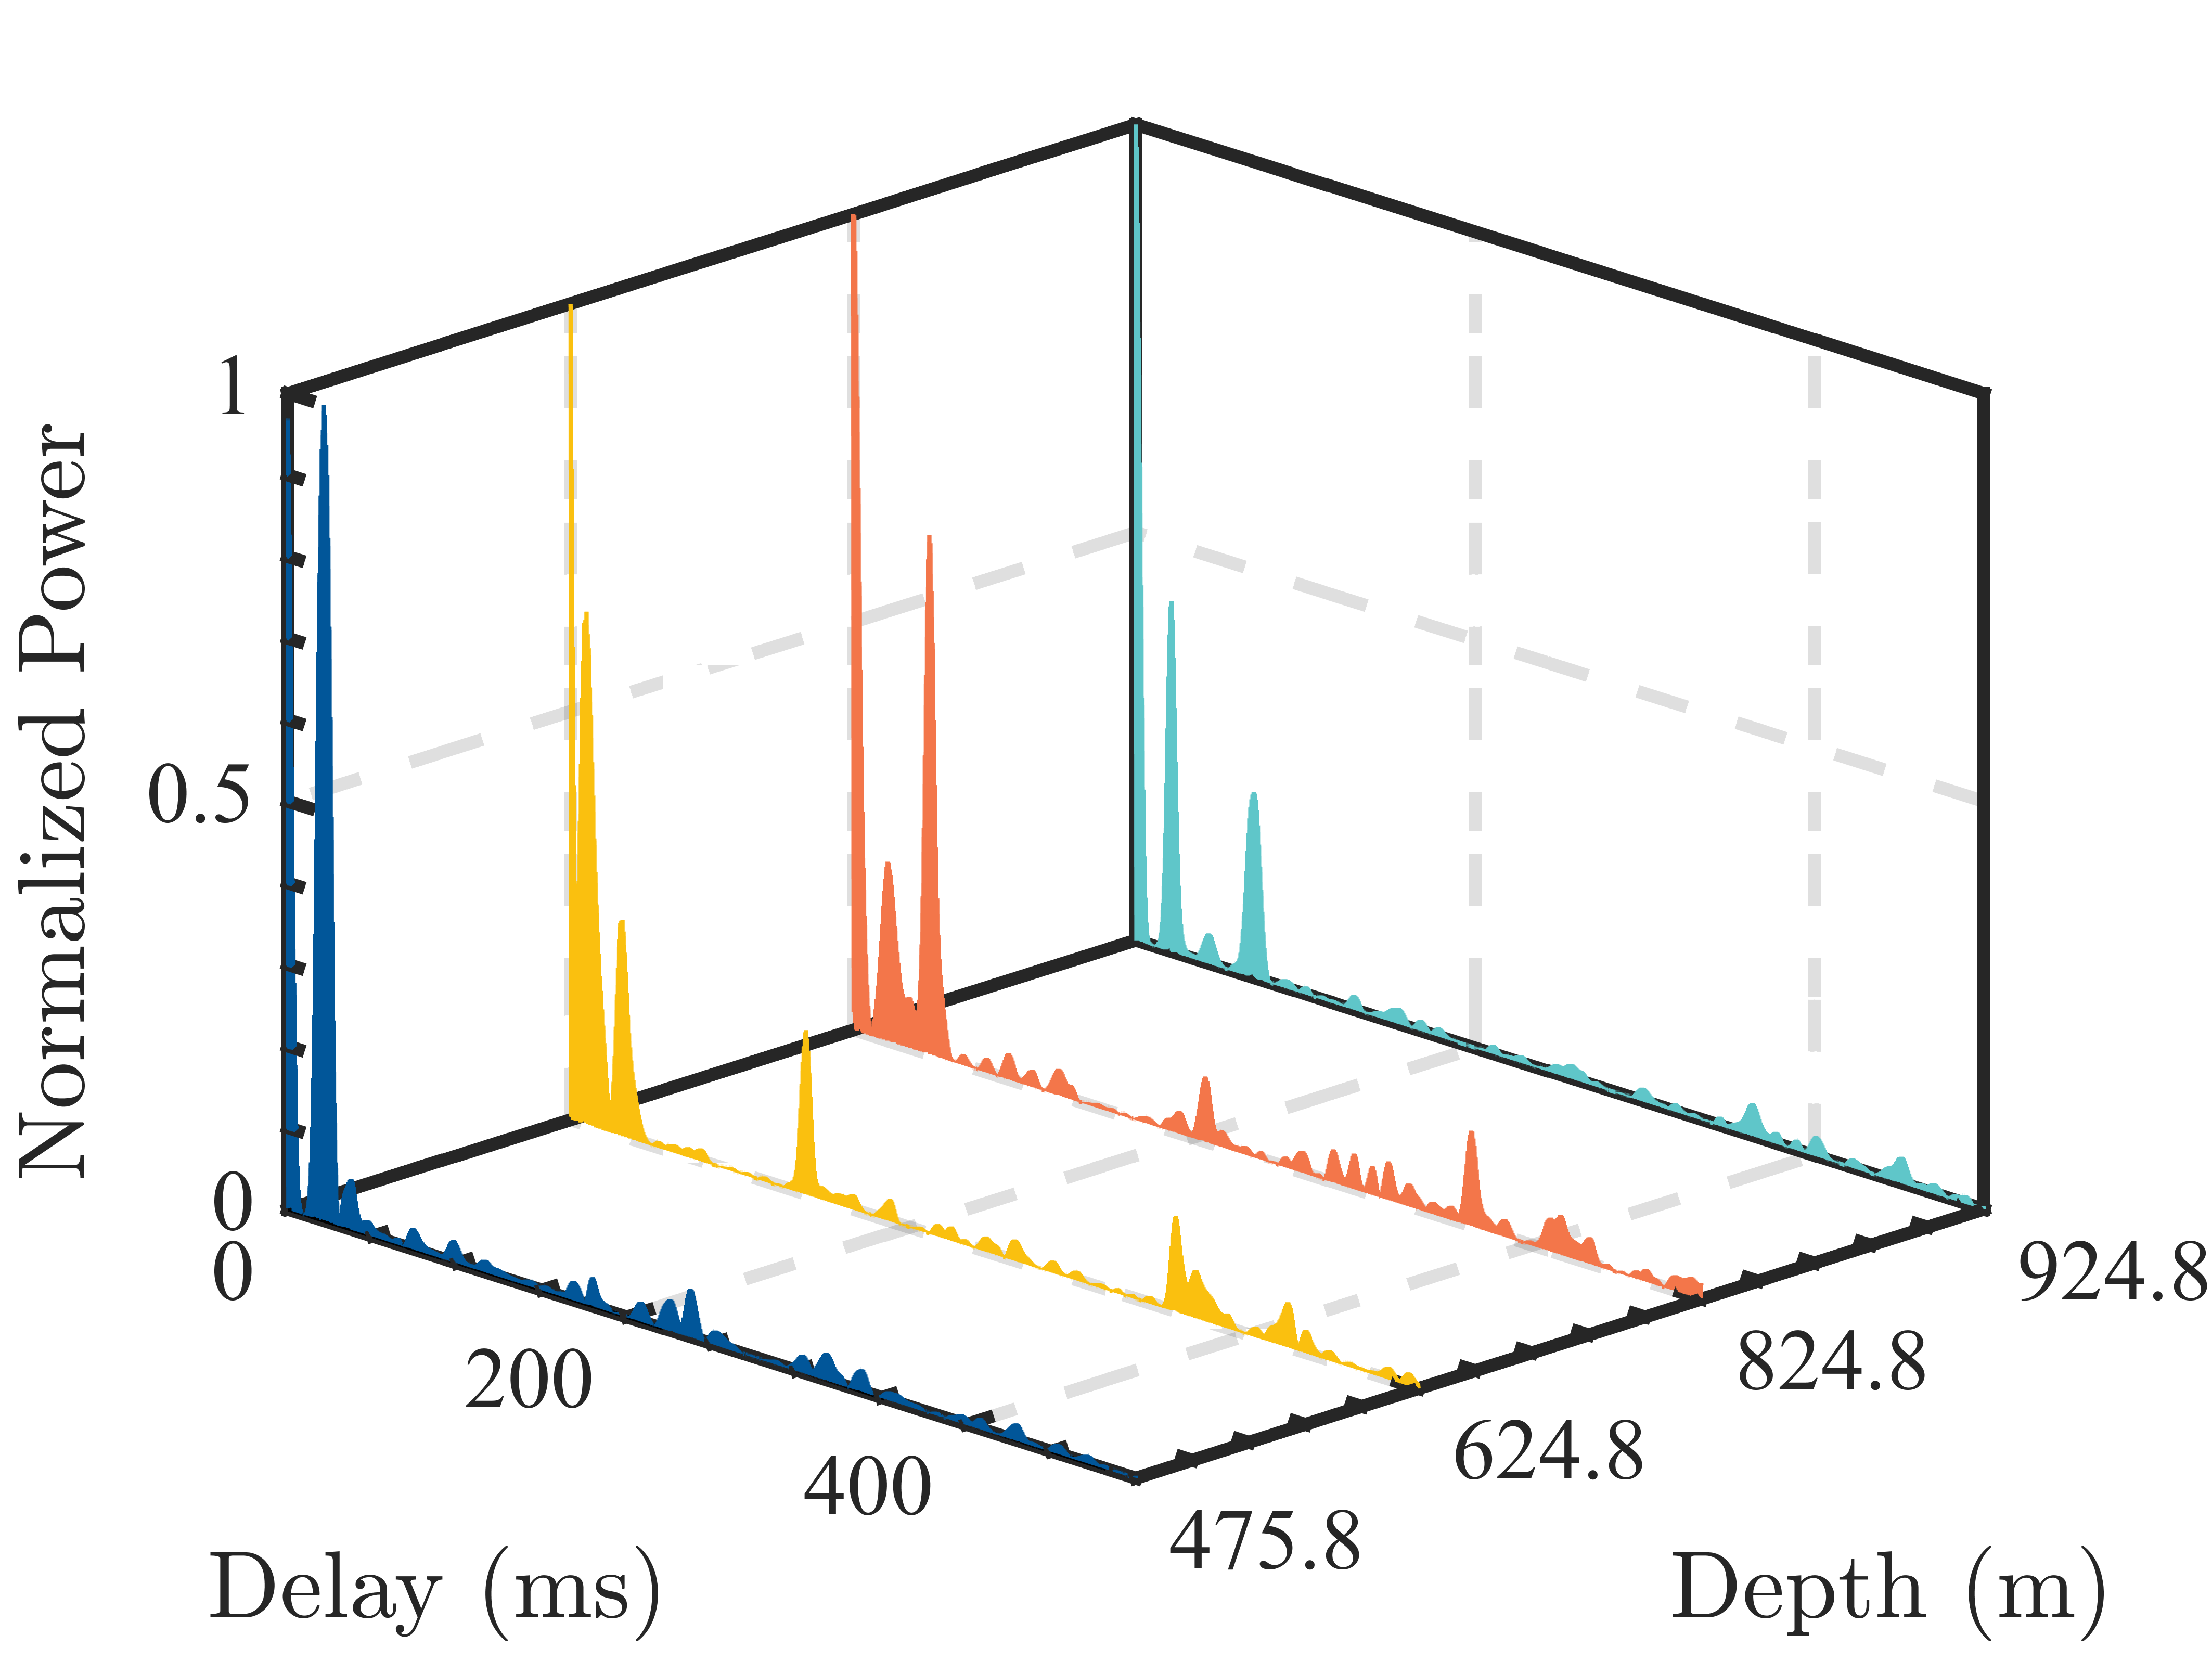
\includegraphics[width=2.5in]{fig/All_power.png}%
\caption{Time-averaged power delay profiles at four receiver depths.}
\label{fig:pdp}
\end{figure}

\subsection{Depth Dependence of Time-Varying Statistics}
\label{subsec:timevar}

Beyond static multipath morphology, channel temporal stability also changes systematically with depth, revealing pronounced deep-layer dynamics that significantly complicate coherent acoustic processing and channel tracking.

\subsubsection{Coherence Time Analysis}

Fig.~\ref{fig:correlation_time} presents the time-interval correlation functions $R_c(\Delta t)$ at all four depths. Their decay rates directly reflect temporal coherence. At 475.8~m, the correlation decays most slowly and remains substantial beyond 1~s, indicating the highest temporal stability among the measured depths.

By contrast, at 824.8~m decorrelation is the fastest, with $|R_c(\Delta t)|$ dropping below 0.5 in about 800~ms. Channel 624.8~m shows intermediate behavior, while 924.8~m exhibits partial stability recovery relative to 824.8~m, although it remains more variable than 475.8~m.

Table~\ref{tab:channel_params} quantifies this behavior via coherence time $T_c$ at thresholds of 0.9 and 0.5. The results show a non-monotonic trend with overall degradation at greater depth. At the 0.5 threshold, $T_c$ is 1003.09~ms, 946.23~ms, 825.59~ms, and 891.59~ms for 475.8~m, 624.8~m, 824.8~m, and 924.8~m, respectively. The minimum at 824.8~m coincides with maximum multipath complexity, indicating the strongest combined impairment from delay dispersion and temporal fluctuation.For a mobile AUV navigating through the main thermocline, this drastic variation in temporal stability poses a critical challenge for adaptive receiver tracking. The rapid channel dynamics at 824.8 m demand aggressive tracking parameters to prevent tracking lag, whereas the high temporal stability at 475.8 m allows for relaxed tracking.

\begin{figure}[!t]
\centering
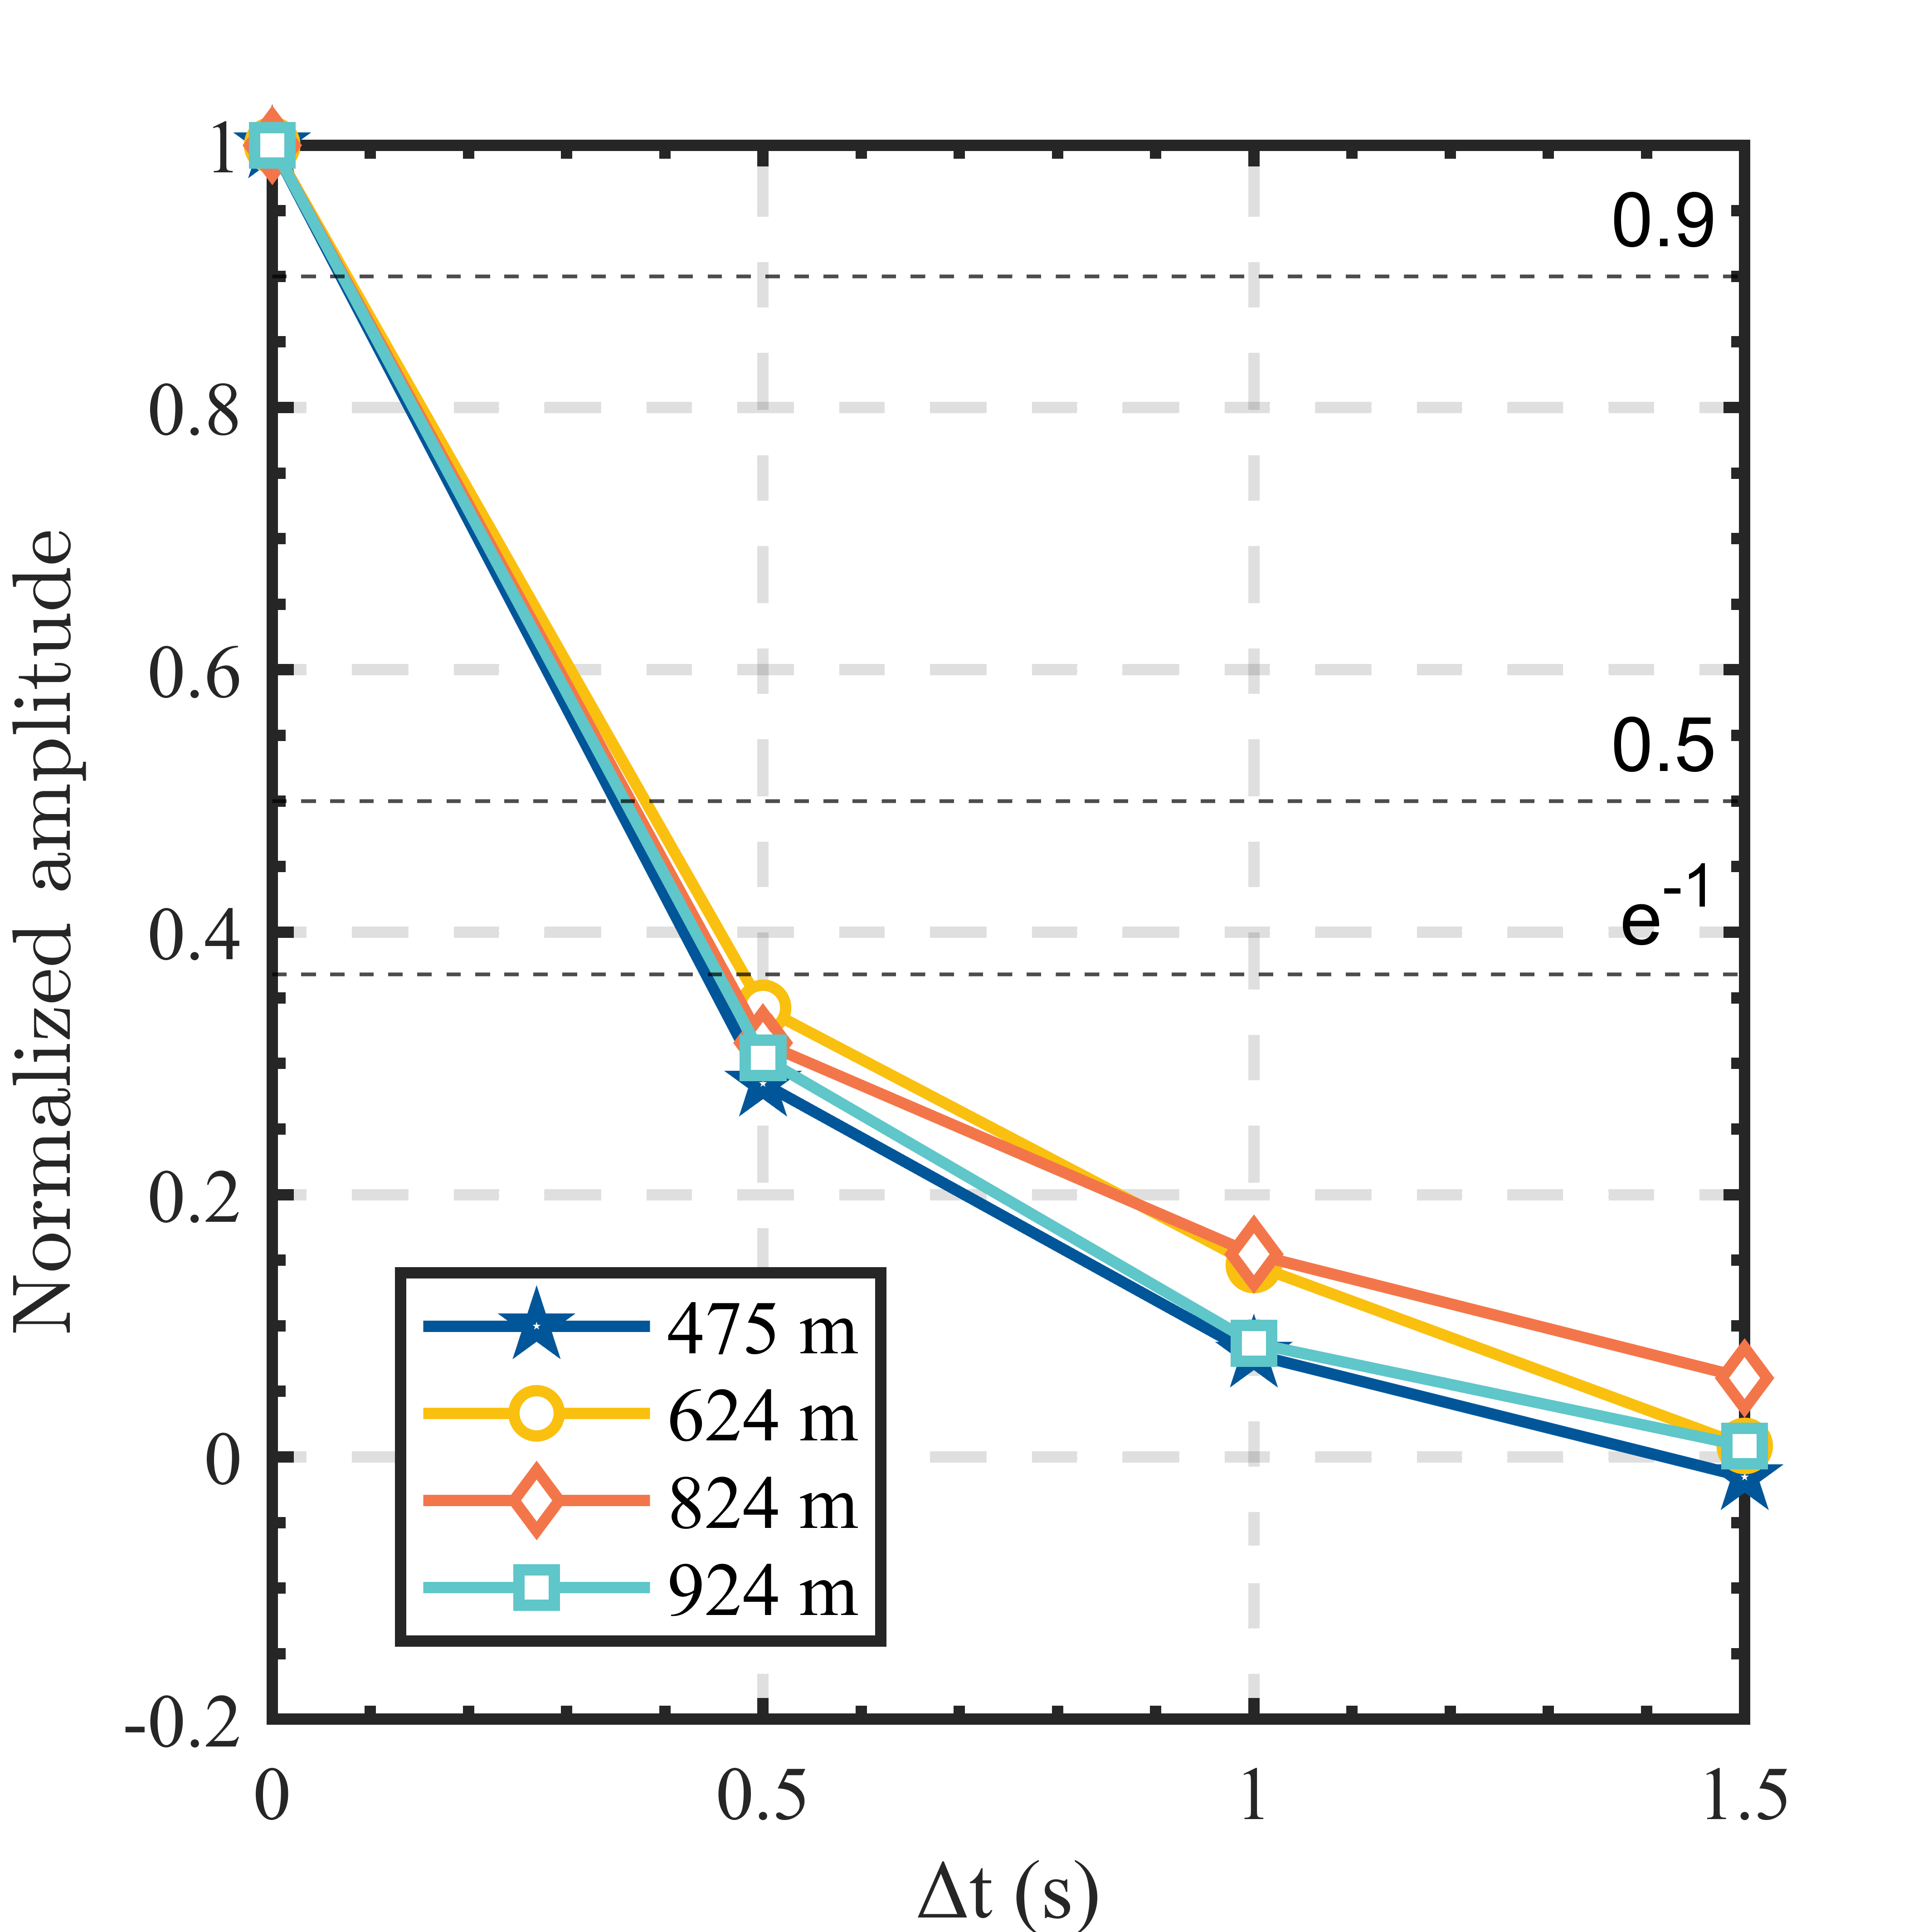
\includegraphics[width=2.5in]{fig/cor_time.png}
\caption{Time-interval correlation functions $|R_c(\Delta t)|$ at four receiver depths.}
\label{fig:correlation_time}
\end{figure}

\subsubsection{Delay Spread Quantification}

Table~\ref{tab:channel_params} also reports mean excess delay $\tau_m$ and RMS delay spread $\tau_{\text{rms}}$ derived from the PDPs. Both follow the same non-monotonic trend: from 98.65~ms and 135.70~ms at 475.8~m, increasing to maxima of 159.70~ms and 160.30~ms at 824.8~m, and then decreasing to 129.34~ms and 152.49~ms at 924.8~m. The nearly 62\% increase in $\tau_m$ and the marked variation in $\tau_{\text{rms}}$ demonstrate the strong impact of receiver depth on ISI severity.

\subsubsection{Frequency Selectivity}

Frequency-domain coherence, represented by coherence bandwidth $B_c$, shows an inverse tendency to delay spread. As listed in Table~\ref{tab:channel_params}, $B_c$ (threshold 0.5) narrows from 0.14~Hz at 475.8~m to 0.11~Hz at 824.8~m, with partial recovery at 924.8~m. This narrowing at mid-depth implies stronger frequency-selective fading and greater equalization demand.

\subsubsection{Doppler Characteristics}

The RMS Doppler spread $\nu_{\text{rms}}$ remains nearly constant across depths (0.024--0.026~Hz), with mean Doppler shifts close to zero, as expected for stationary platforms. This indicates that depth-dependent coherence differences are not driven primarily by bulk Doppler magnitude, but by multipath-structure-dependent sensitivity to environmental fluctuation, discussed further in Section~\ref{sec:mechanism}.

\begin{table*}[!t]
\renewcommand{\arraystretch}{1.2}
\caption{Key Channel Parameters at Different Receiver Depths}
\label{tab:channel_params}
\centering
\begin{tabular}{|c|c|c|c|c|c|c|}
\hline
\textbf{Depth (m)} & \boldmath{$\tau_m$} \textbf{(ms)} & \boldmath{$\tau_{\text{rms}}$} \textbf{(ms)} & \boldmath{$T_{c,0.9}$} \textbf{(ms)} & \boldmath{$T_{c,0.5}$} \textbf{(ms)} & \boldmath{$B_{c,0.5}$} \textbf{(Hz)} & \boldmath{$\nu_{\text{rms}}$} \textbf{(Hz)} \\
\hline
475.8 & 98.65 & 135.70 & 1258.34 & 1003.09 & 0.14 & 0.024 \\
\hline
624.8 & 113.79 & 155.22 & 1264.78 & 946.23 & 0.13 & 0.025 \\
\hline
824.8 & \textbf{159.70} & \textbf{160.30} & 1204.82 & \textbf{825.59} & \textbf{0.11} & 0.026 \\
\hline
924.8 & 129.34 & 152.49 & 1228.07 & 891.59 & 0.11 & 0.026 \\
\hline
\end{tabular}
\\[3pt]
Note: Subscripts denote correlation thresholds. Boldface indicates extremal values.
\end{table*}

\subsection{Breakdown of Classical Channel Relationships}
\label{subsec:breakdown}

Classical wireless channel theory often assumes approximate inverse relationships between coherence bandwidth and RMS delay spread ($B_c \propto 1/\tau_{\text{rms}}$), and between coherence time and RMS Doppler spread ($T_c \propto 1/\nu_{\text{rms}}$). Our measurements show that these relationships are insufficient for deep sea UWA channel characterization\cite{ref20}.

Fig.~\ref{fig:classical_breakdown} illustrates the relationships between key parameters, revealing clear deviations in both instances. For $B_c$--$\tau_{\text{rms}}$, the mismatch is attributable to the sparse, discrete, and clustered multipath structure: $\tau_{\text{rms}}$ (a second central moment) is highly sensitive to weak long-delay tails, whereas $B_c$ is governed mainly by interference among dominant arrivals. Consequently, the presence of a low-power path with a large delay can significantly increase $\tau_{\text{rms}}$ while leaving $B_c$ relatively unchanged, thus challenging the universality of  this relationship. In our data, the 824.8~m channel has the largest $\tau_{\text{rms}}$, yet $B_c$ does not decrease proportionally because the extended tail carries a weak, weakly coherent energy.

For $T_c$--$\nu_{\text{rms}}$, near-constant $\nu_{\text{rms}}$ across depths contrasts with substantial $T_c$ variation. This decoupling indicates that deep sea temporal coherence is controlled less by bulk Doppler spread and more by phase stability of dominant refracted paths under dynamic sound-speed structure, which is not captured by first-order Doppler statistics.

These results imply that deep sea UWA channels cannot be adequately parameterized by $\tau_{\text{rms}}$ and $\nu_{\text{rms}}$ alone. Accurate modeling and performance prediction require explicit treatment of path sparsity, dominant-path stability, and depth-dependent environmental coupling.

\begin{figure}[!t]
\centering
\subfloat[]{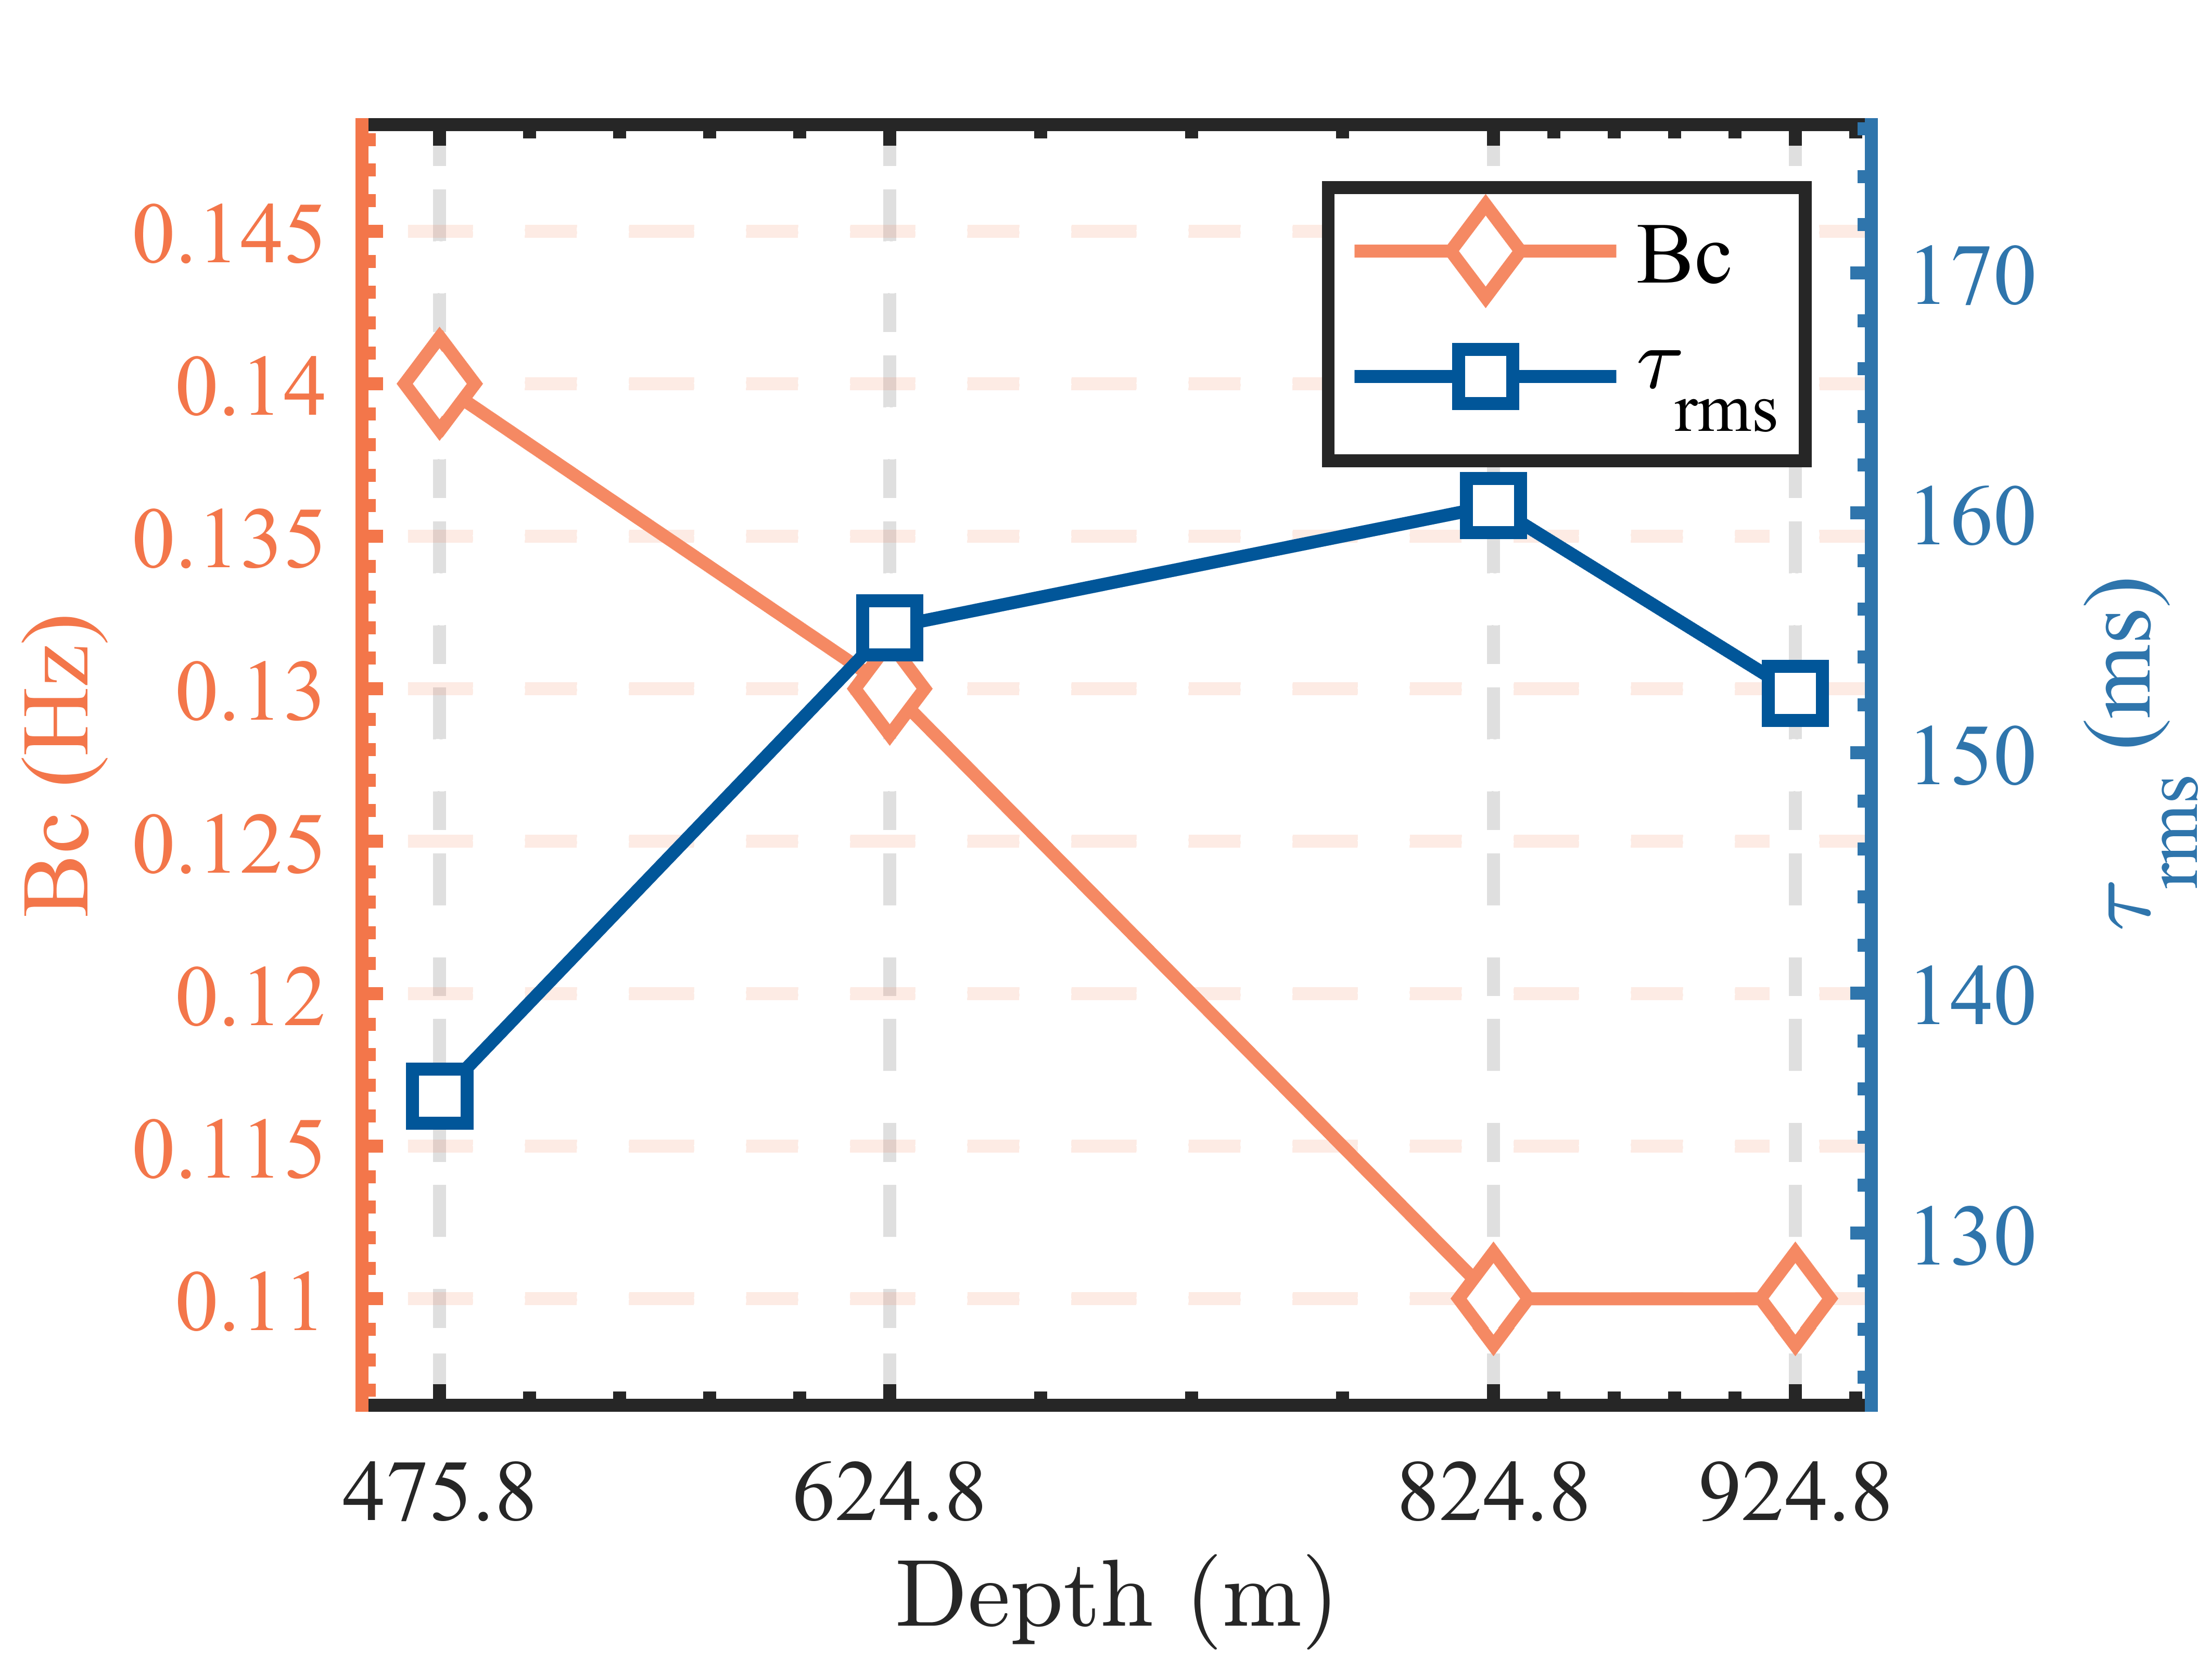
\includegraphics[width=2.5in]{fig/Bc_tau_rms2.png}
\label{fig:bc_tau}}
\hfill
\subfloat[]{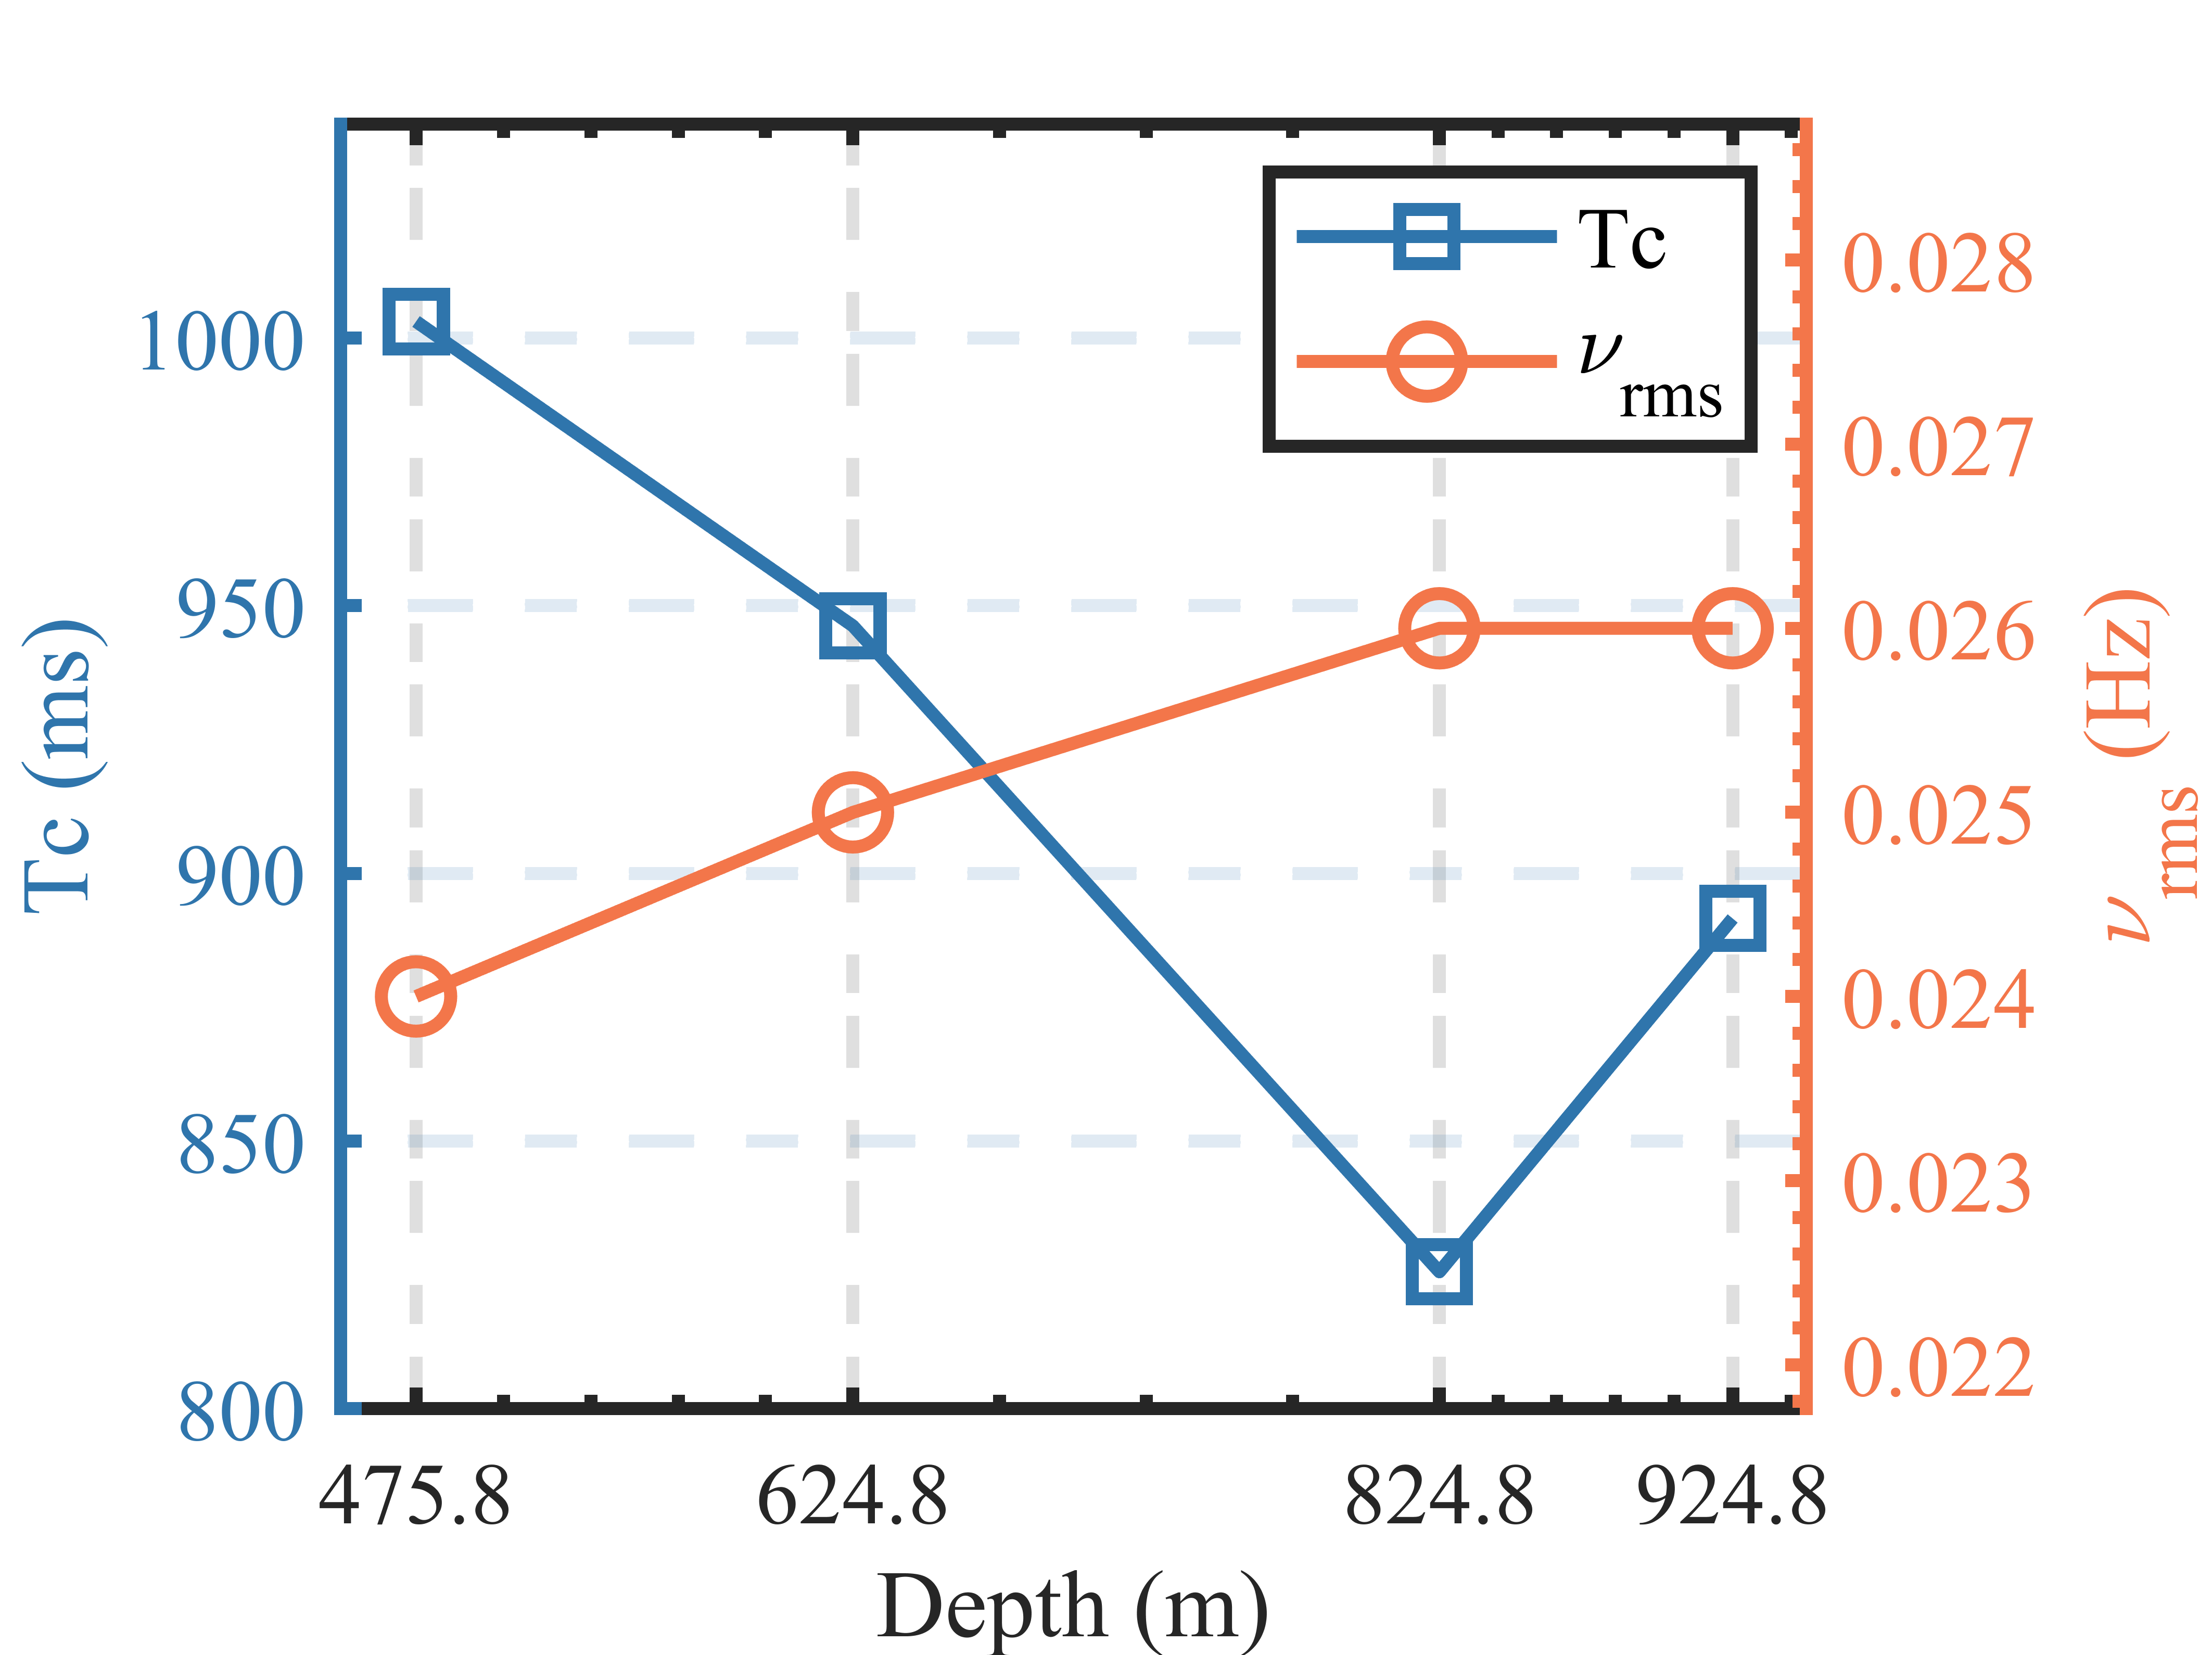
\includegraphics[width=2.5in]{fig/Tc_f_rms.png}
\label{fig:tc_nu}}
\caption{Deviation from classical channel relationships: (a) measured $B_c$ vs. $\tau_{\text{rms}}$; (b) measured $T_c$ vs. $\nu_{\text{rms}}$ .}
\label{fig:classical_breakdown}
\end{figure}


The results above establish three key points: (i) deep sea channel characteristics exhibit strong non-monotonic depth dependence, with mid-depths near 825~m forming the most challenging operating region; (ii) temporal variability increases in deeper layers, contrary to common intuition; and (iii) classical RF-style channel relationships break down in this sparse multipath regime. These findings motivate the physical interpretation and system-level analysis presented in Section~\ref{sec:mechanism}.


\section{Vehicular Receiver Optimization Based on Physical Insights}
\label{sec:mechanism}

The experimental results in Section~\ref{sec:results} reveal pronounced depth-dependent variation in deep sea channel characteristics, with the most challenging conditions occurring near mid-depths around 825~m. This section first interprets these observations using acoustic-propagation physics and then translates them into concrete receiver-design implications through quantitative system-level analysis.

\subsection{Channel Modeling for AUV Trajectories Across Thermoclines}

\subsubsection{Multipath Structure Evolution and Acoustic Focusing}

\begin{figure*}[!t]
\centering
\subfloat[]{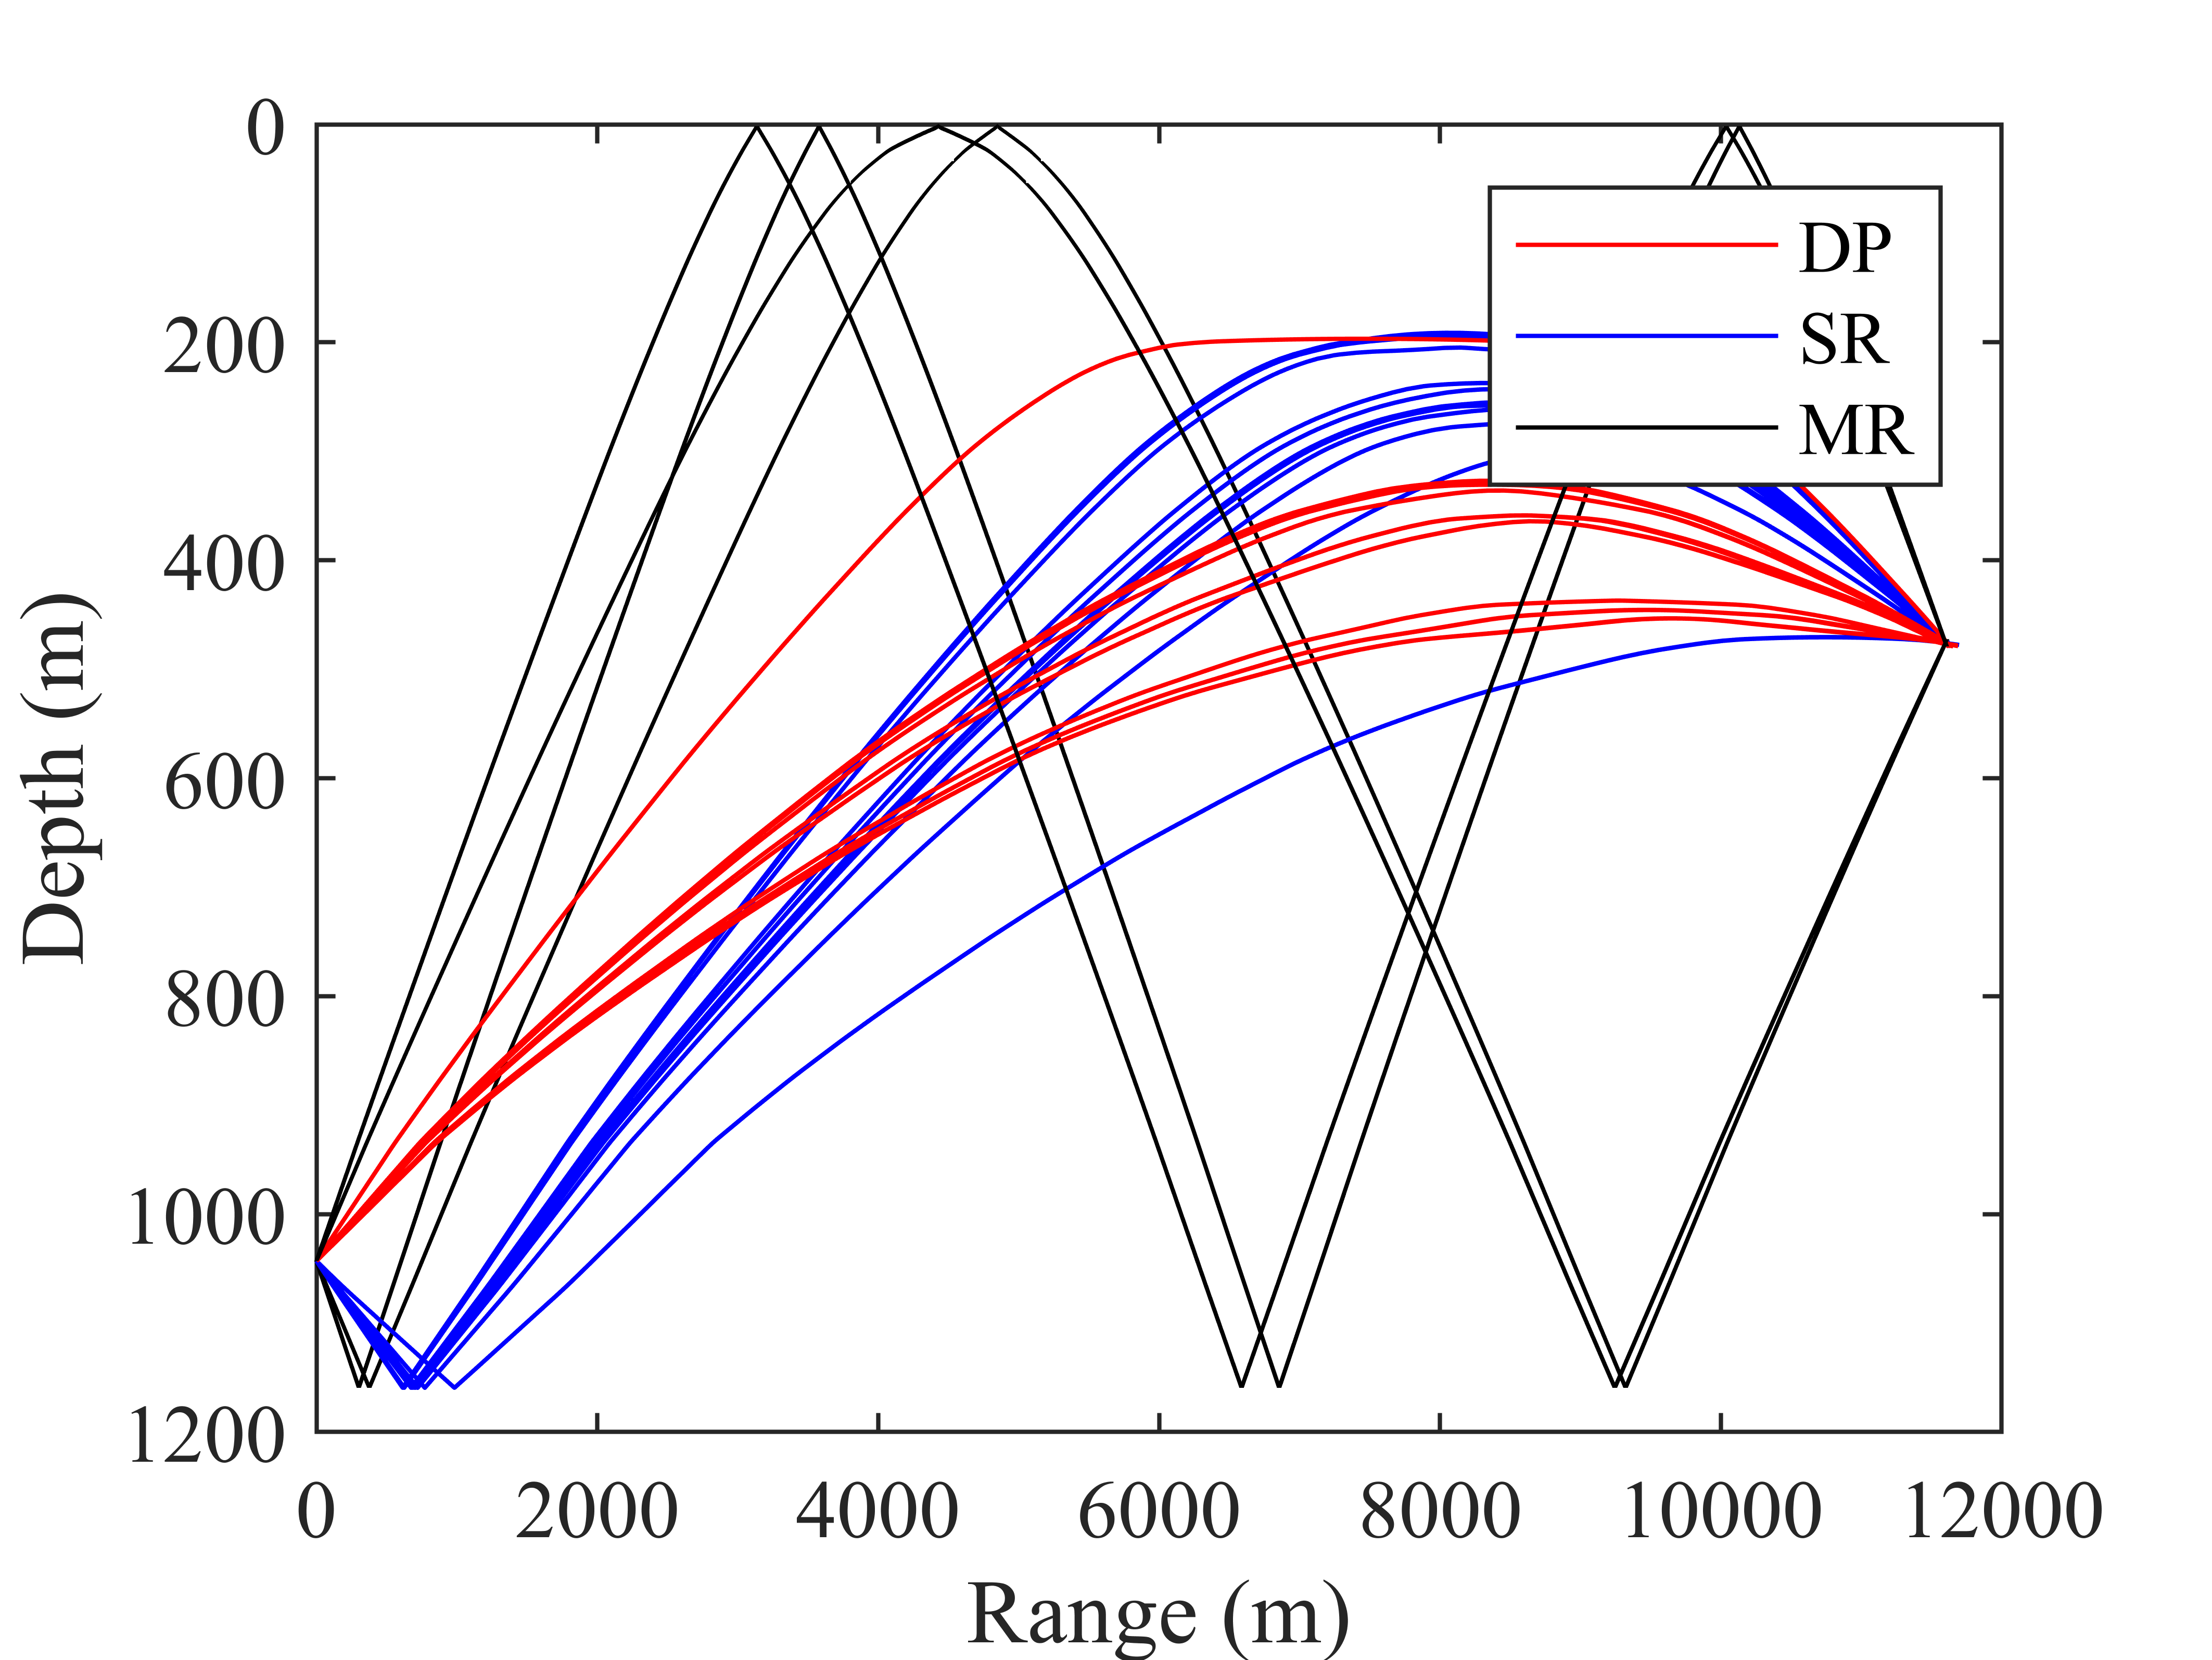
\includegraphics[width=2.5in]{fig/ray_475.png}
\label{raytrace_first}}
\hfil
\subfloat[]{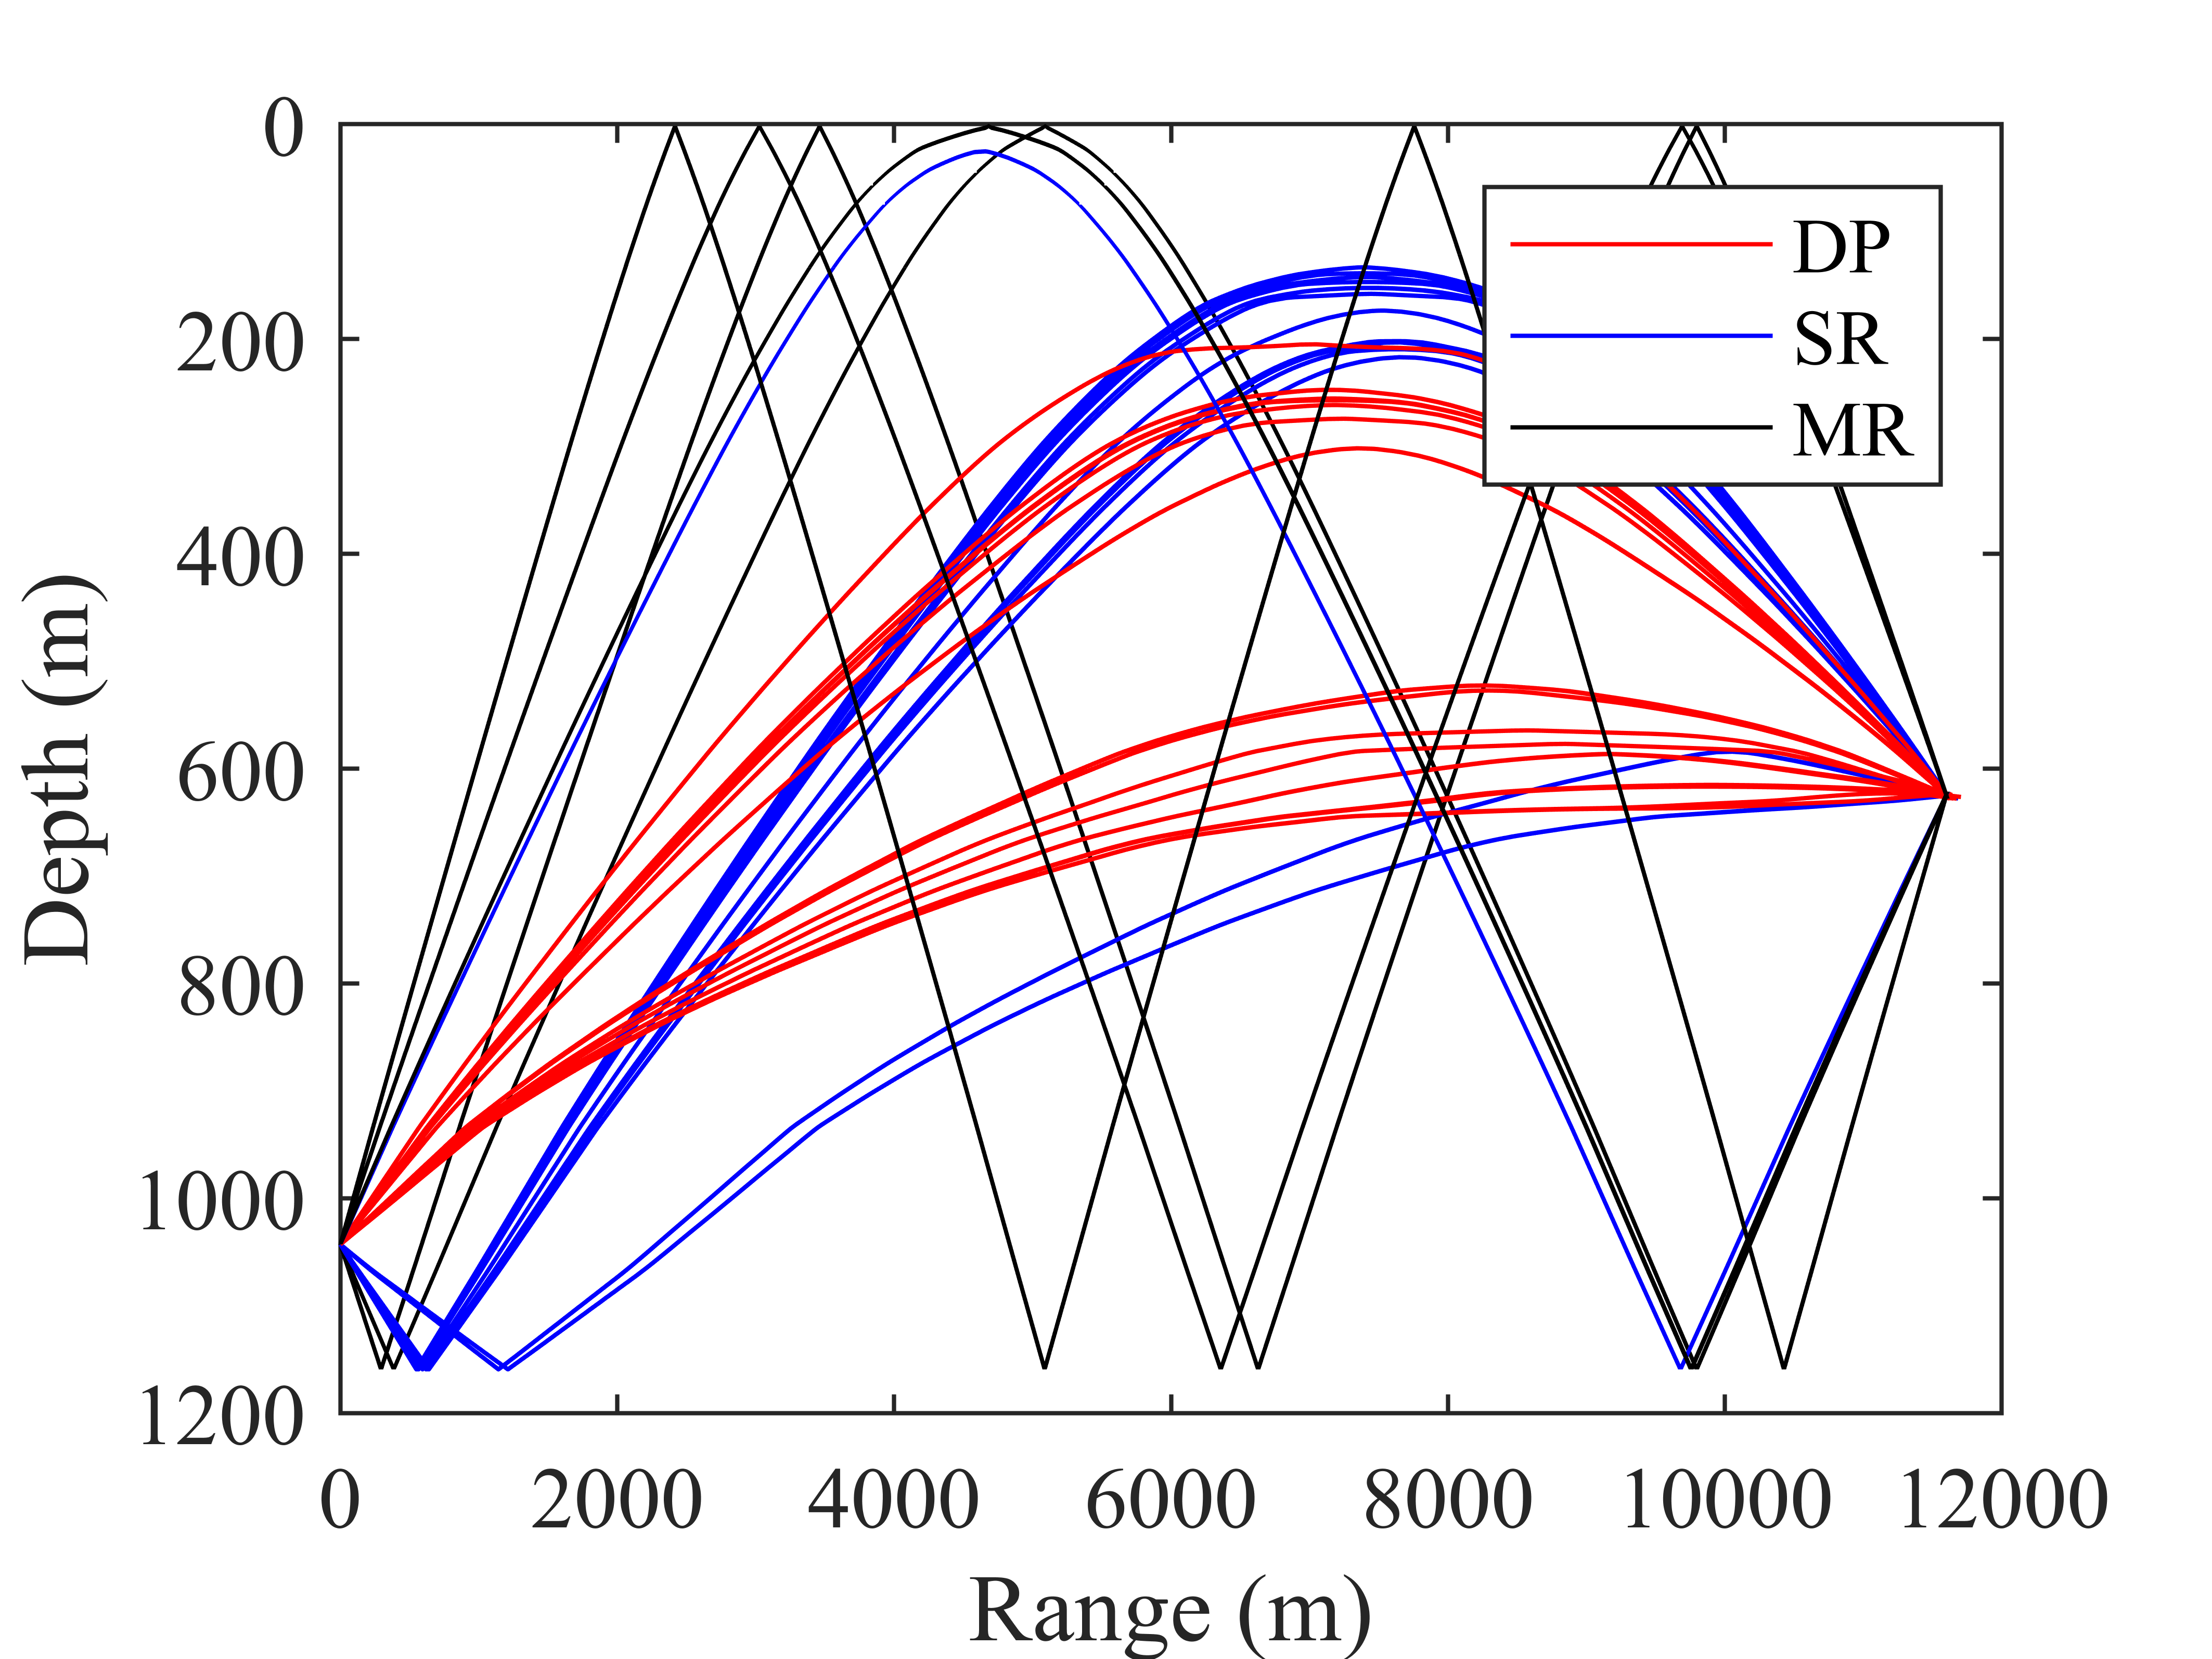
\includegraphics[width=2.5in]{fig/ray_624.png}
\label{raytrace_second}}
\\
\subfloat[]{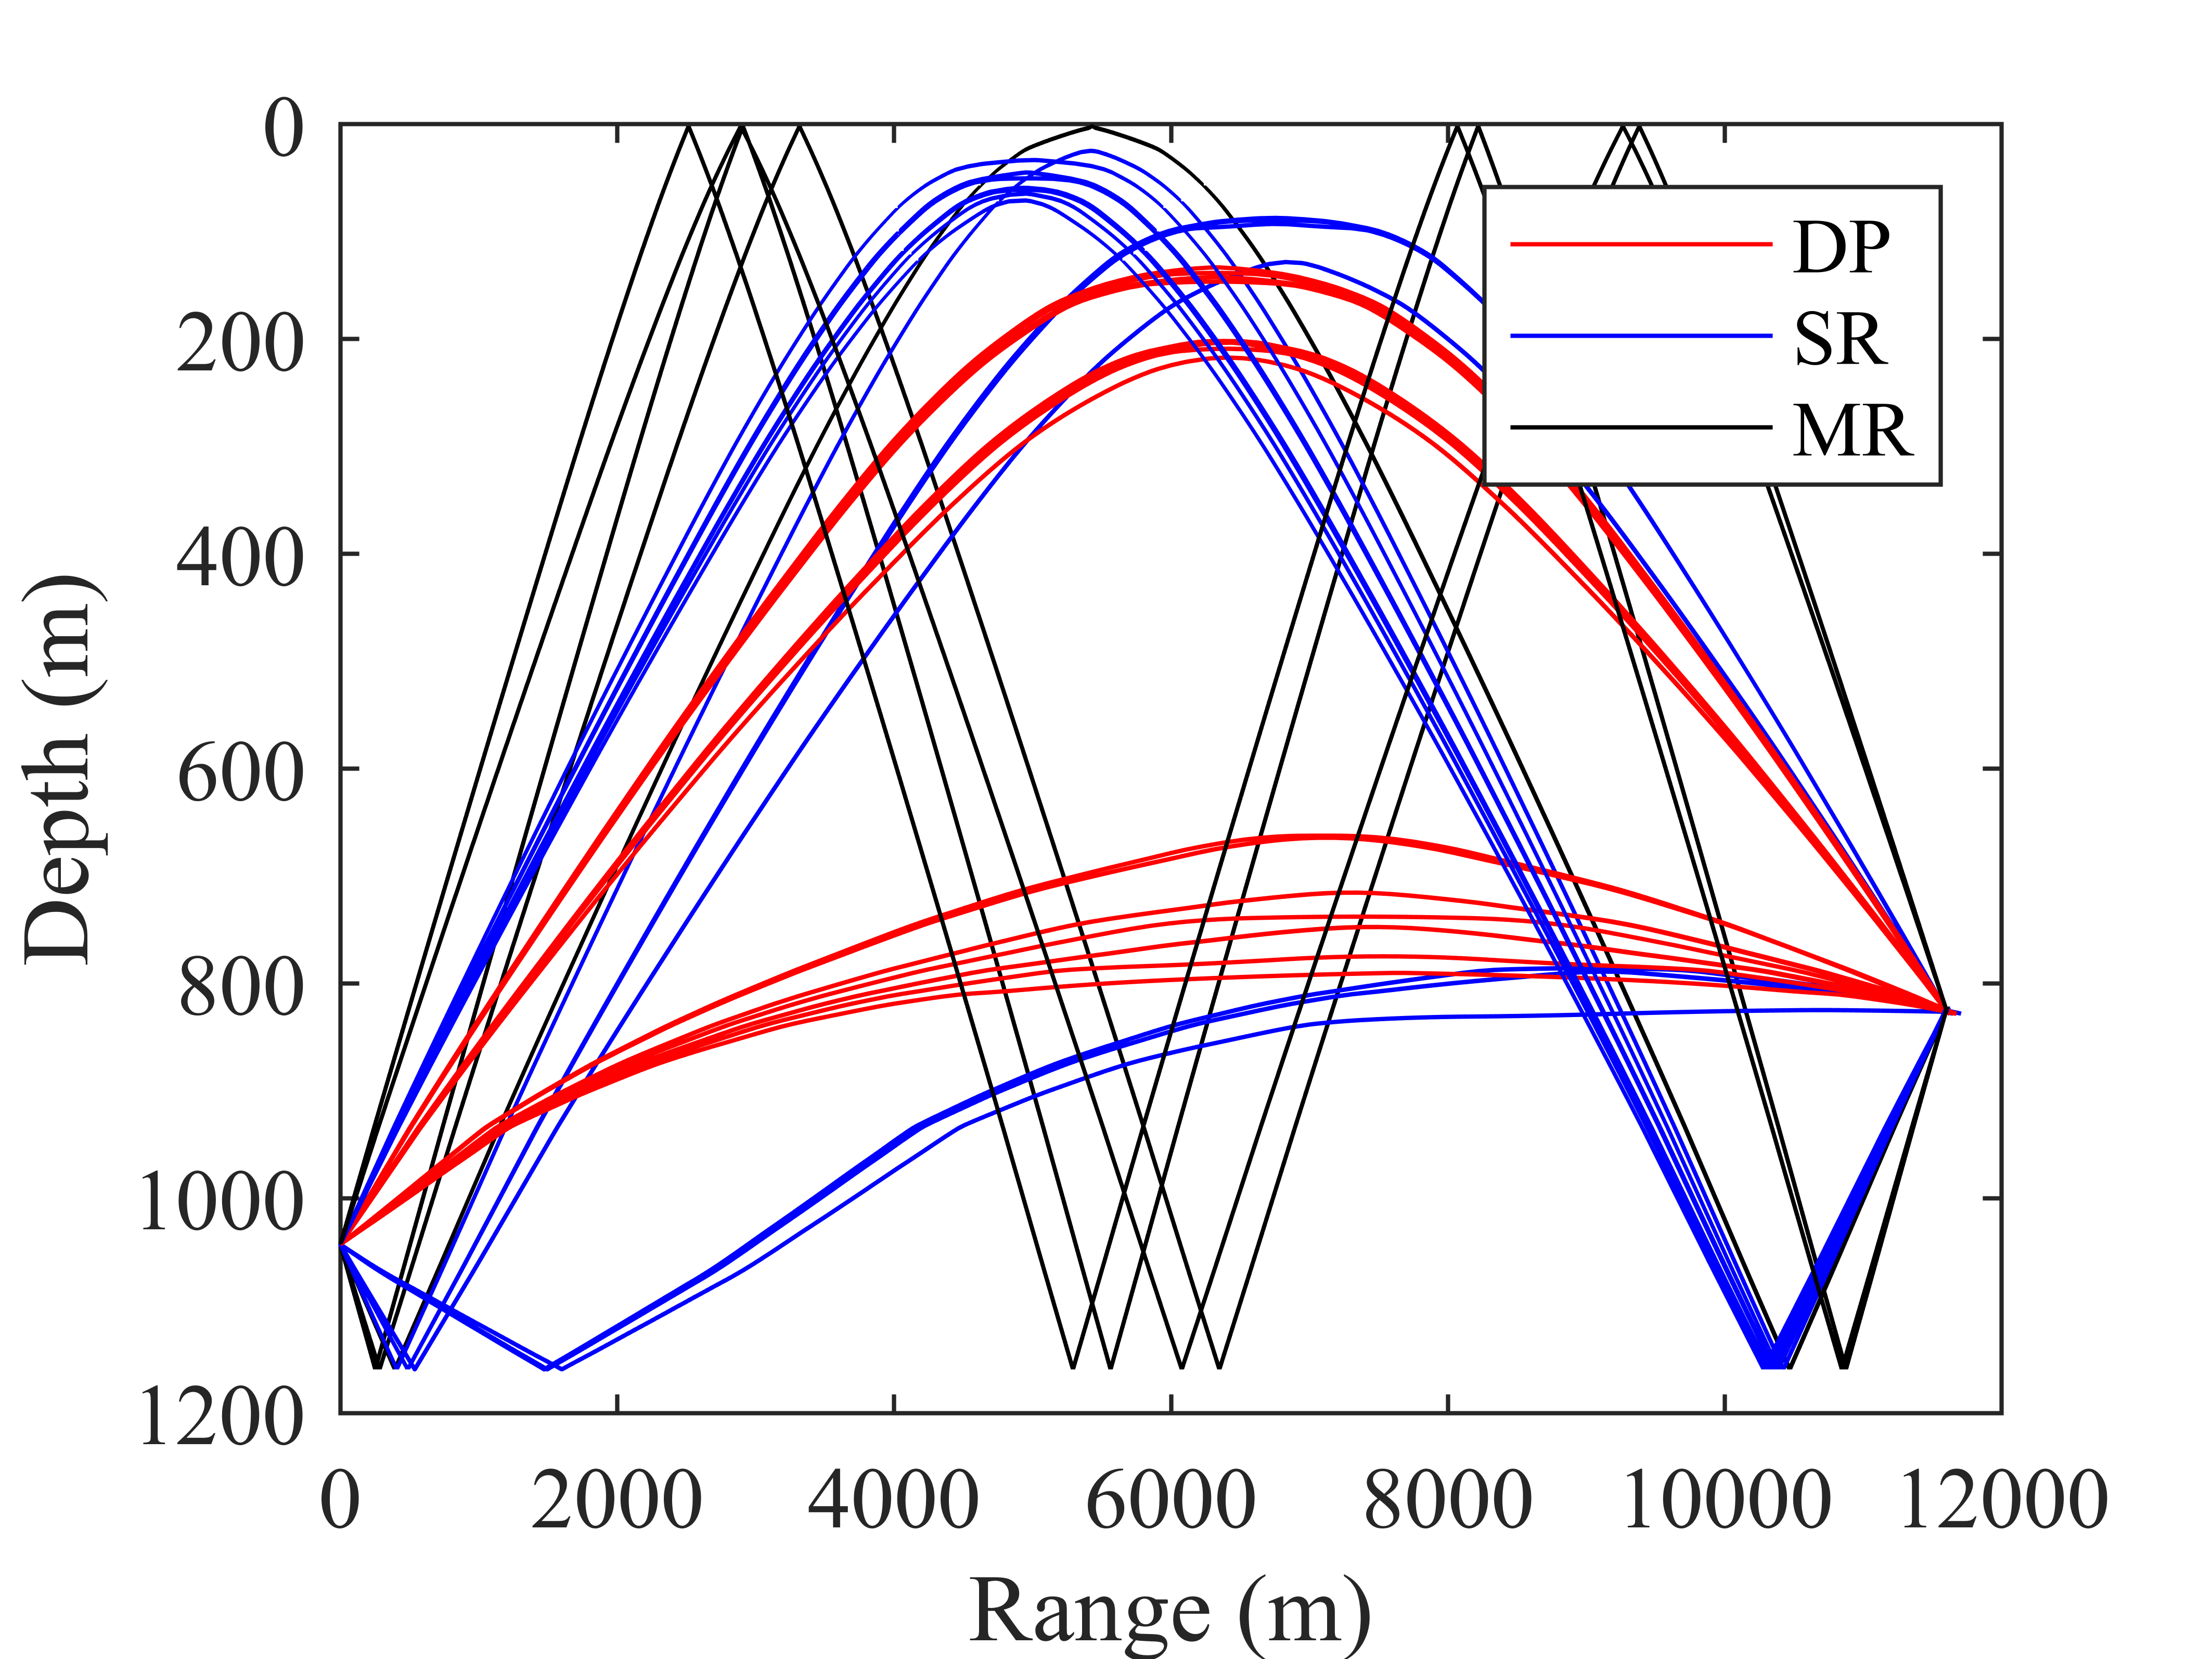
\includegraphics[width=2.5in]{fig/ray_824.png}
\label{raytrace_third}}
\hfil
\subfloat[]{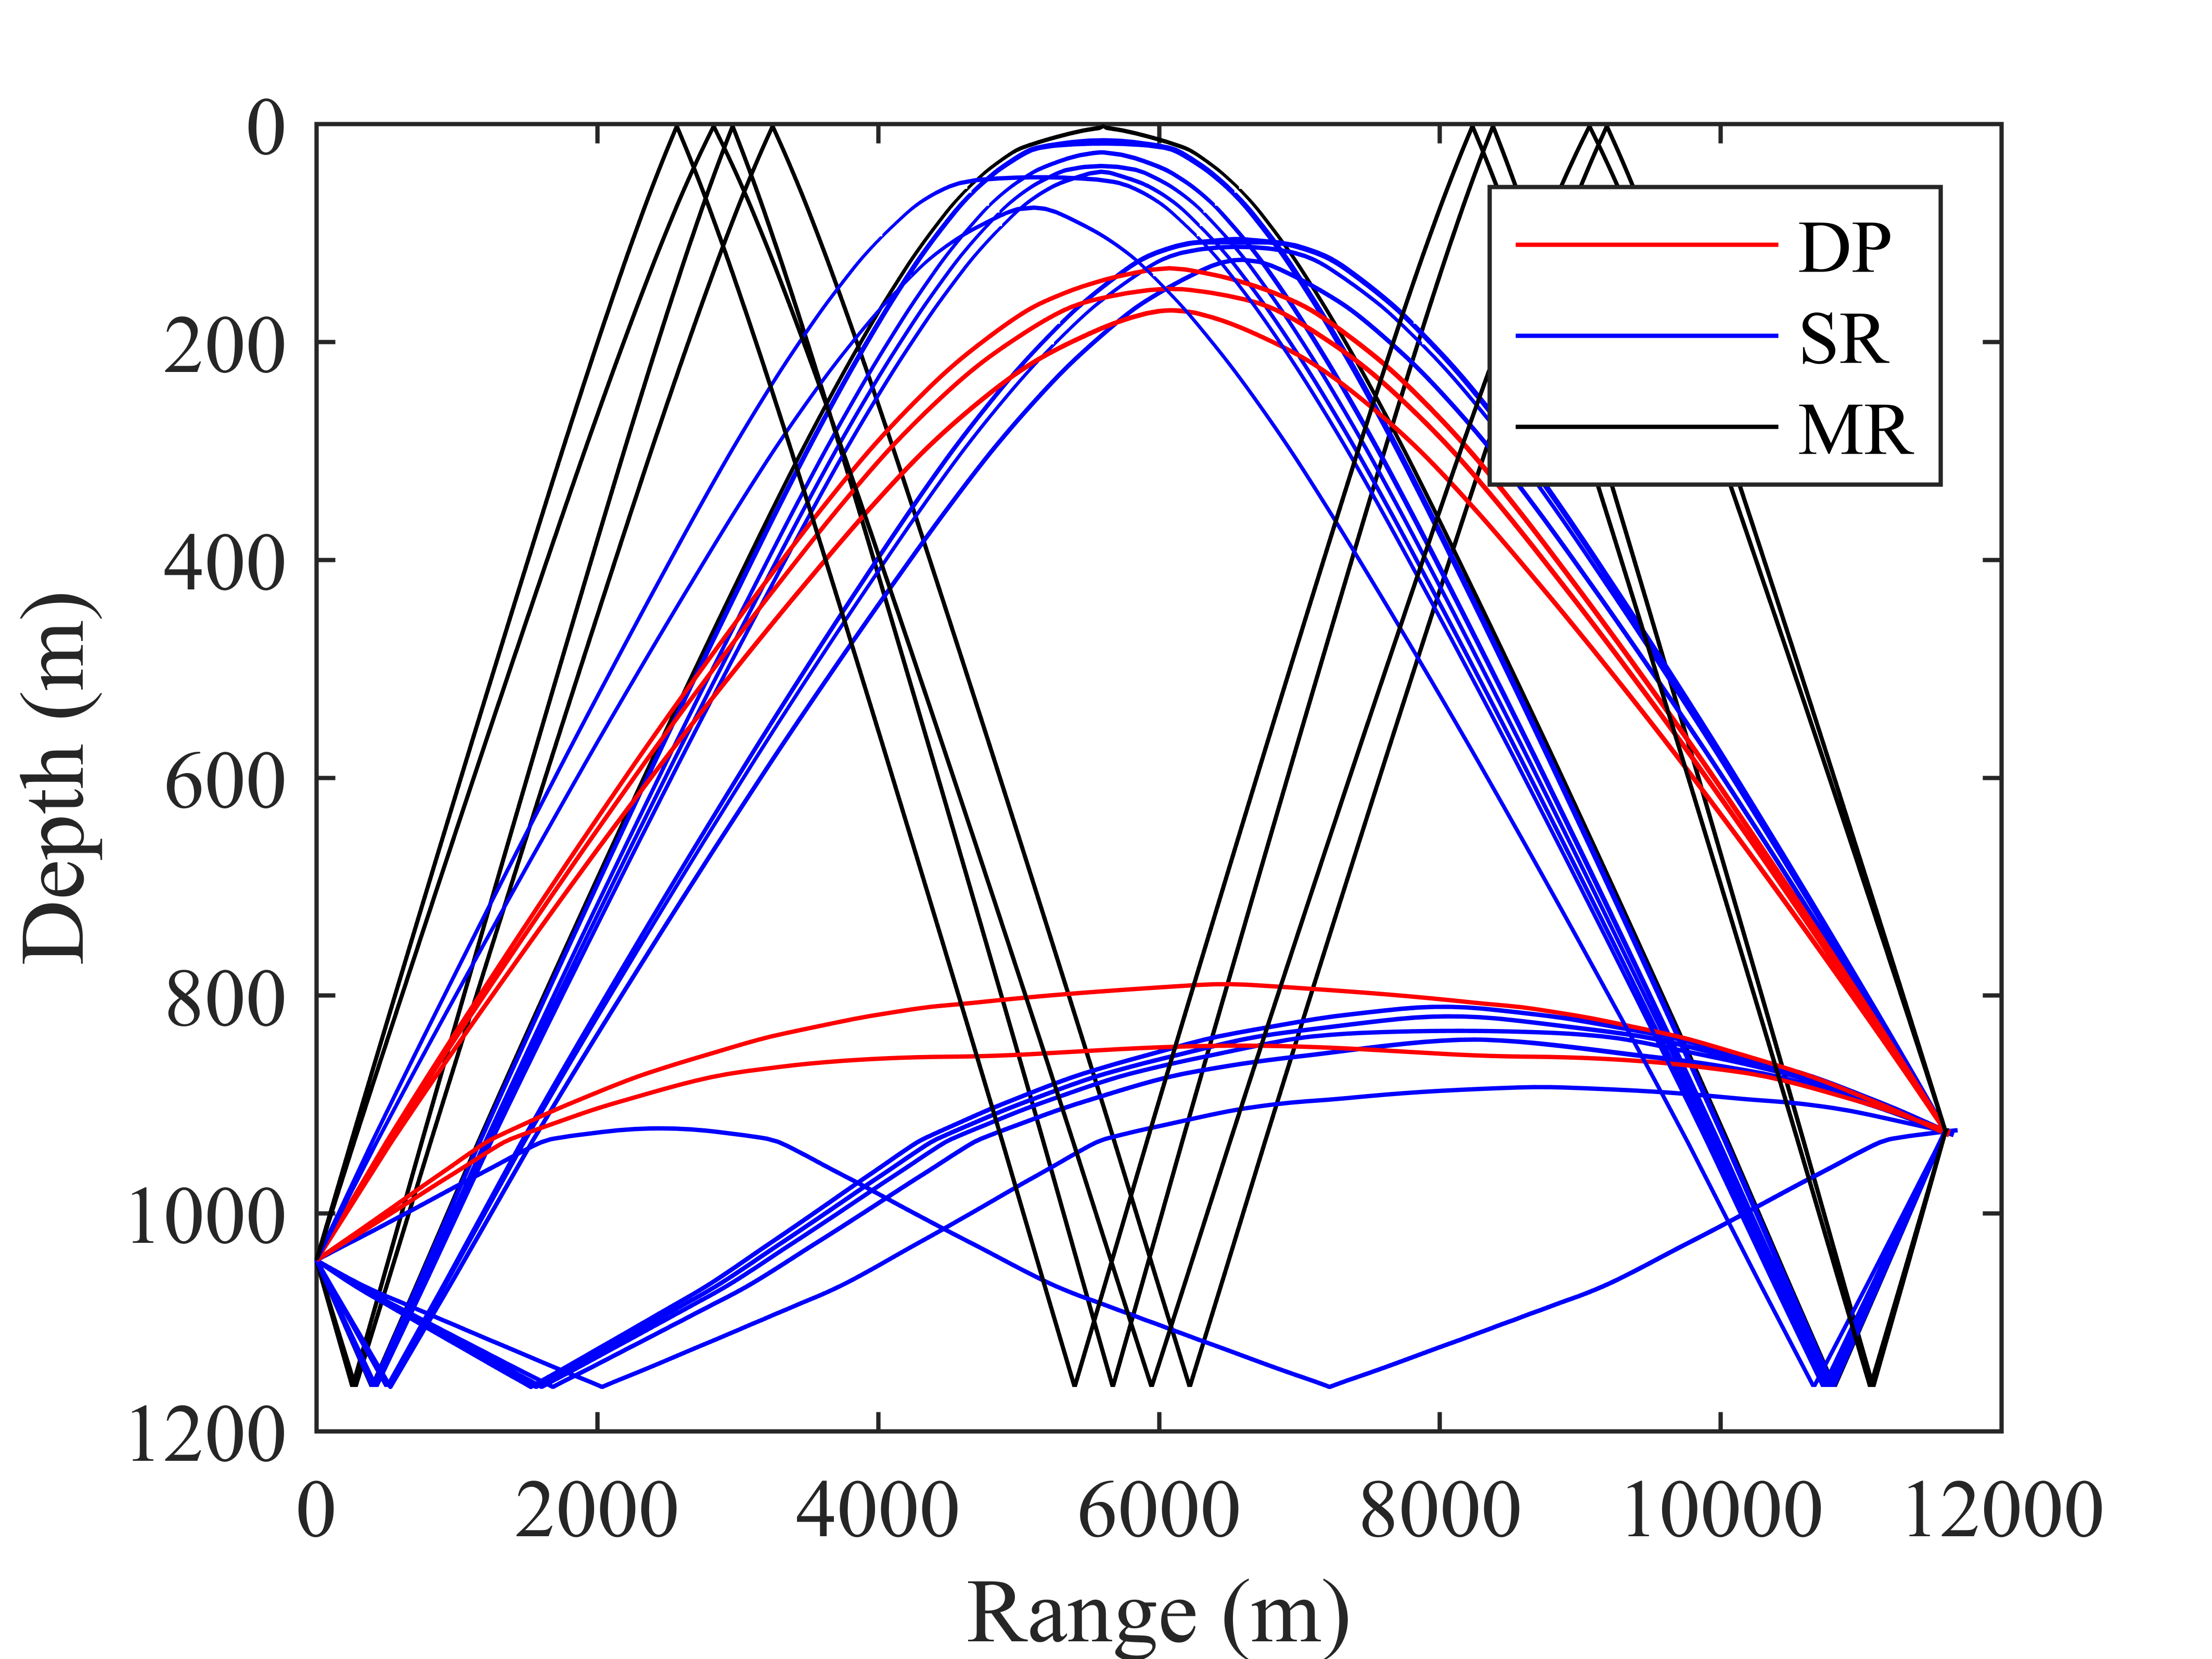
\includegraphics[width=2.5in]{fig/ray_924.png}
\label{raytrace_forth}}
\caption{Eigenray diagrams simulated using the Bellhop ray-tracing model at four depths: (a) 475.8~m, (b) 624.8~m, (c) 824.8~m, (d) 924.8~m.}
\label{fig:raytrace}
\end{figure*}

The non-monotonic multipath evolution, with peak RMS delay spread occurring in the lower main thermocline (824.8~m) rather than at the deepest receiver, is attributable to coupled effects of sound-speed structure and geometric spreading. As shown in Fig.~\ref{fig:ssp}, the measured SSP follows a typical deep-ocean pattern: a seasonal thermocline layer, a main thermocline extending to about 1000~m, and an underlying deep isothermal layer. The source was deployed at 1043~m within the deep isothermal layer, whereas the VLA spanned the lower thermocline.

In the upper main thermocline  (475.8~m), the channel remains relatively simple, dominated by direct transmission with limited boundary-reflected components. As receiver depth increases, stronger vertical sound-speed gradients intensify refraction, producing more complex eigenray trajectories with additional boundary interactions and internal bending. The maximum complexity at 824.8~m coincides with a refractive-convergence region associated with upward focusing from the deep sound-channel axis (SOFAR axis), which the SSP indicates is near 900--1000~m. This convergence generates caustic focusing and explains the observed energy inversion, where the third arrival exceeds the second (Fig.~\ref{fig:pdp}).


To verify this interpretation, we performed Bellhop ray-tracing simulations using the measured SSP. Fig.~\ref{fig:raytrace} shows eigenray patterns at four representative depths, demonstrating a transition from sparse propagation dominated by direct and single-reflection rays at 475.8~m to dense focused multipath at 824.8~m, followed by a simplified seabed-influenced structure at 924.8~m.



\subsubsection{Enhanced Time-Variability in Deep Layers}

The counterintuitive result that coherence time decreases with depth, indicating stronger temporal variability in deeper channels, requires careful interpretation. Although surface forcing (wind waves and swell) is often treated as the dominant driver of UWA channel dynamics, even our shallowest hydrophone (475.8~m) is well below the layer of direct surface agitation.

Instead, the enhanced deep-layer variability is best explained by cumulative phase sensitivity of long-delay eigenrays to deep-ocean dynamics. Internal waves, mesoscale eddies, and thermohaline intrusions perturb the SSP microstructure \cite{ref21}, significantly affecting acoustic variability and the arrival structure of the CIR modeled via ray tracing\cite{ref22}. Although these perturbations are small in amplitude, they accumulate substantial phase error over long refracted paths. At 824.8~m, where energy is distributed among many arrivals (Fig.~\ref{fig:pdp}), interference becomes highly sensitive to such phase perturbations, causing rapid decorrelation. By contrast, the 475.8~m channel is dominated by fewer and more stable paths and therefore preserves longer coherence. The partial coherence recovery at 924.8~m is consistent with seabed absorption simplifying the multipath field by suppressing weaker interfering components.

\subsection{Implications for Equalizer Design: Coping with Multipath}
\label{subsec:equalizer}

\begin{figure*}[!t]
\centering
\subfloat[]{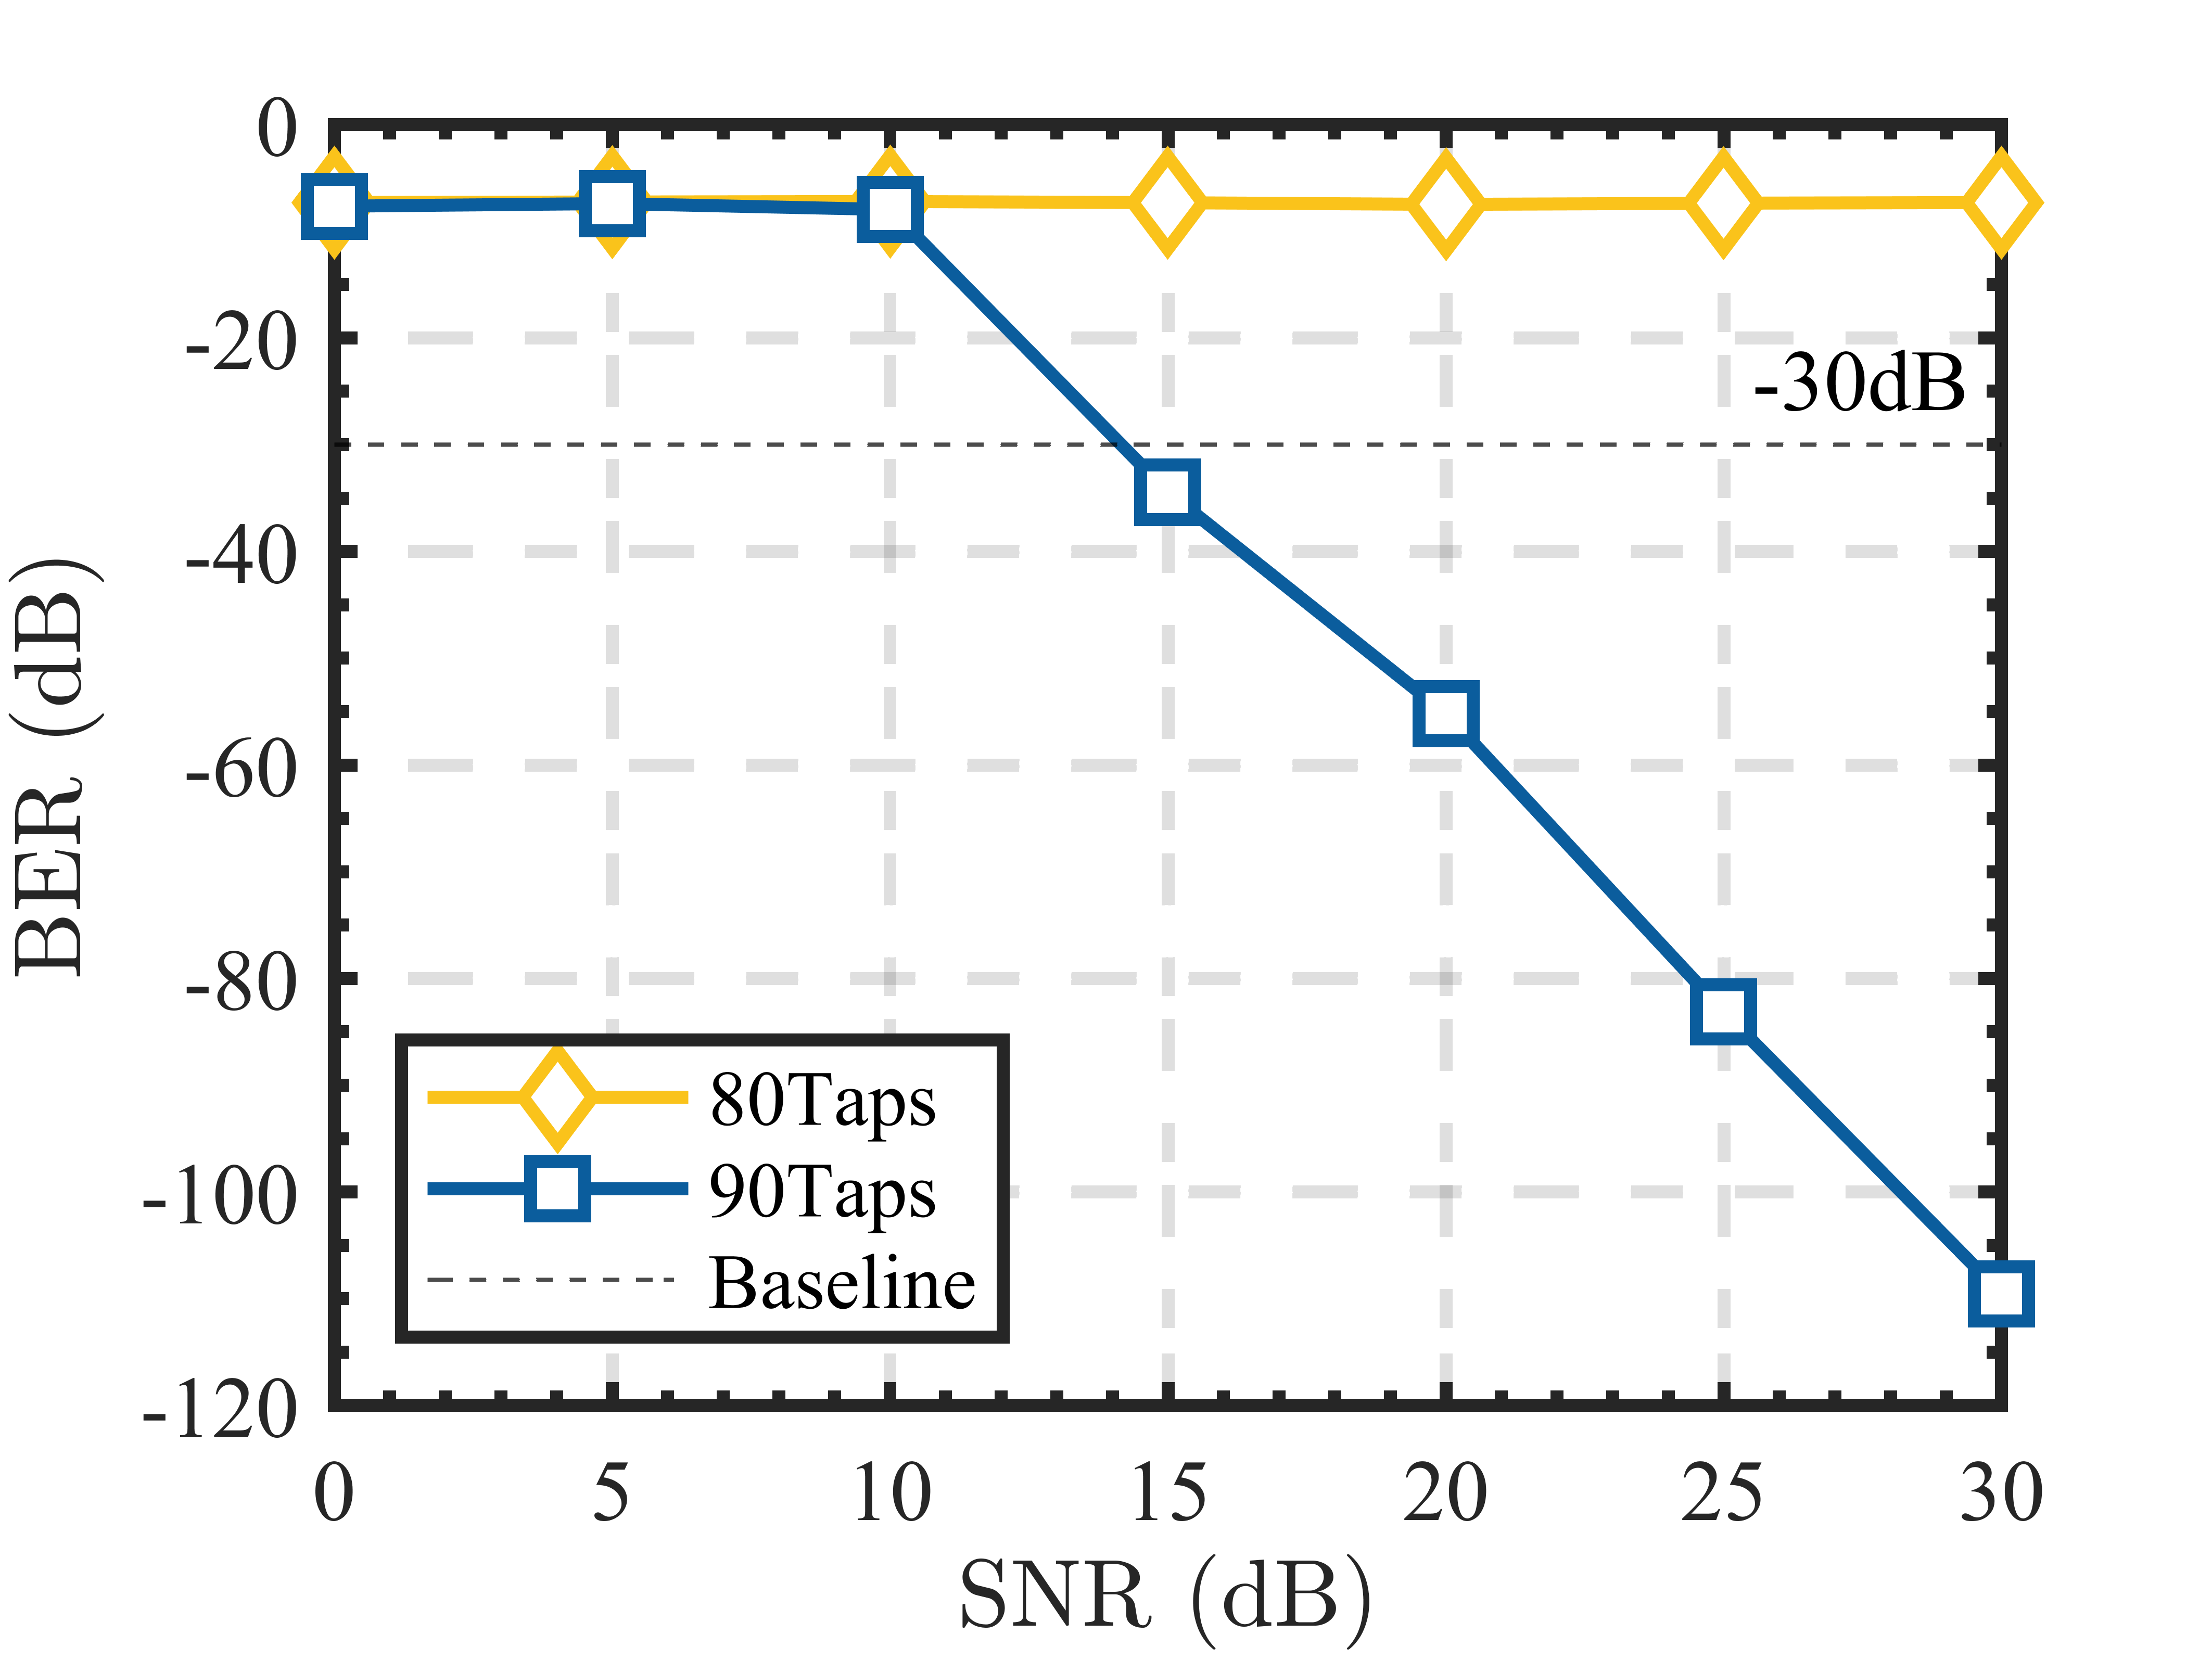
\includegraphics[width=2.5in]{fig/Taps_475.png}
\label{ber_taps_first}}
\hfil
\subfloat[]{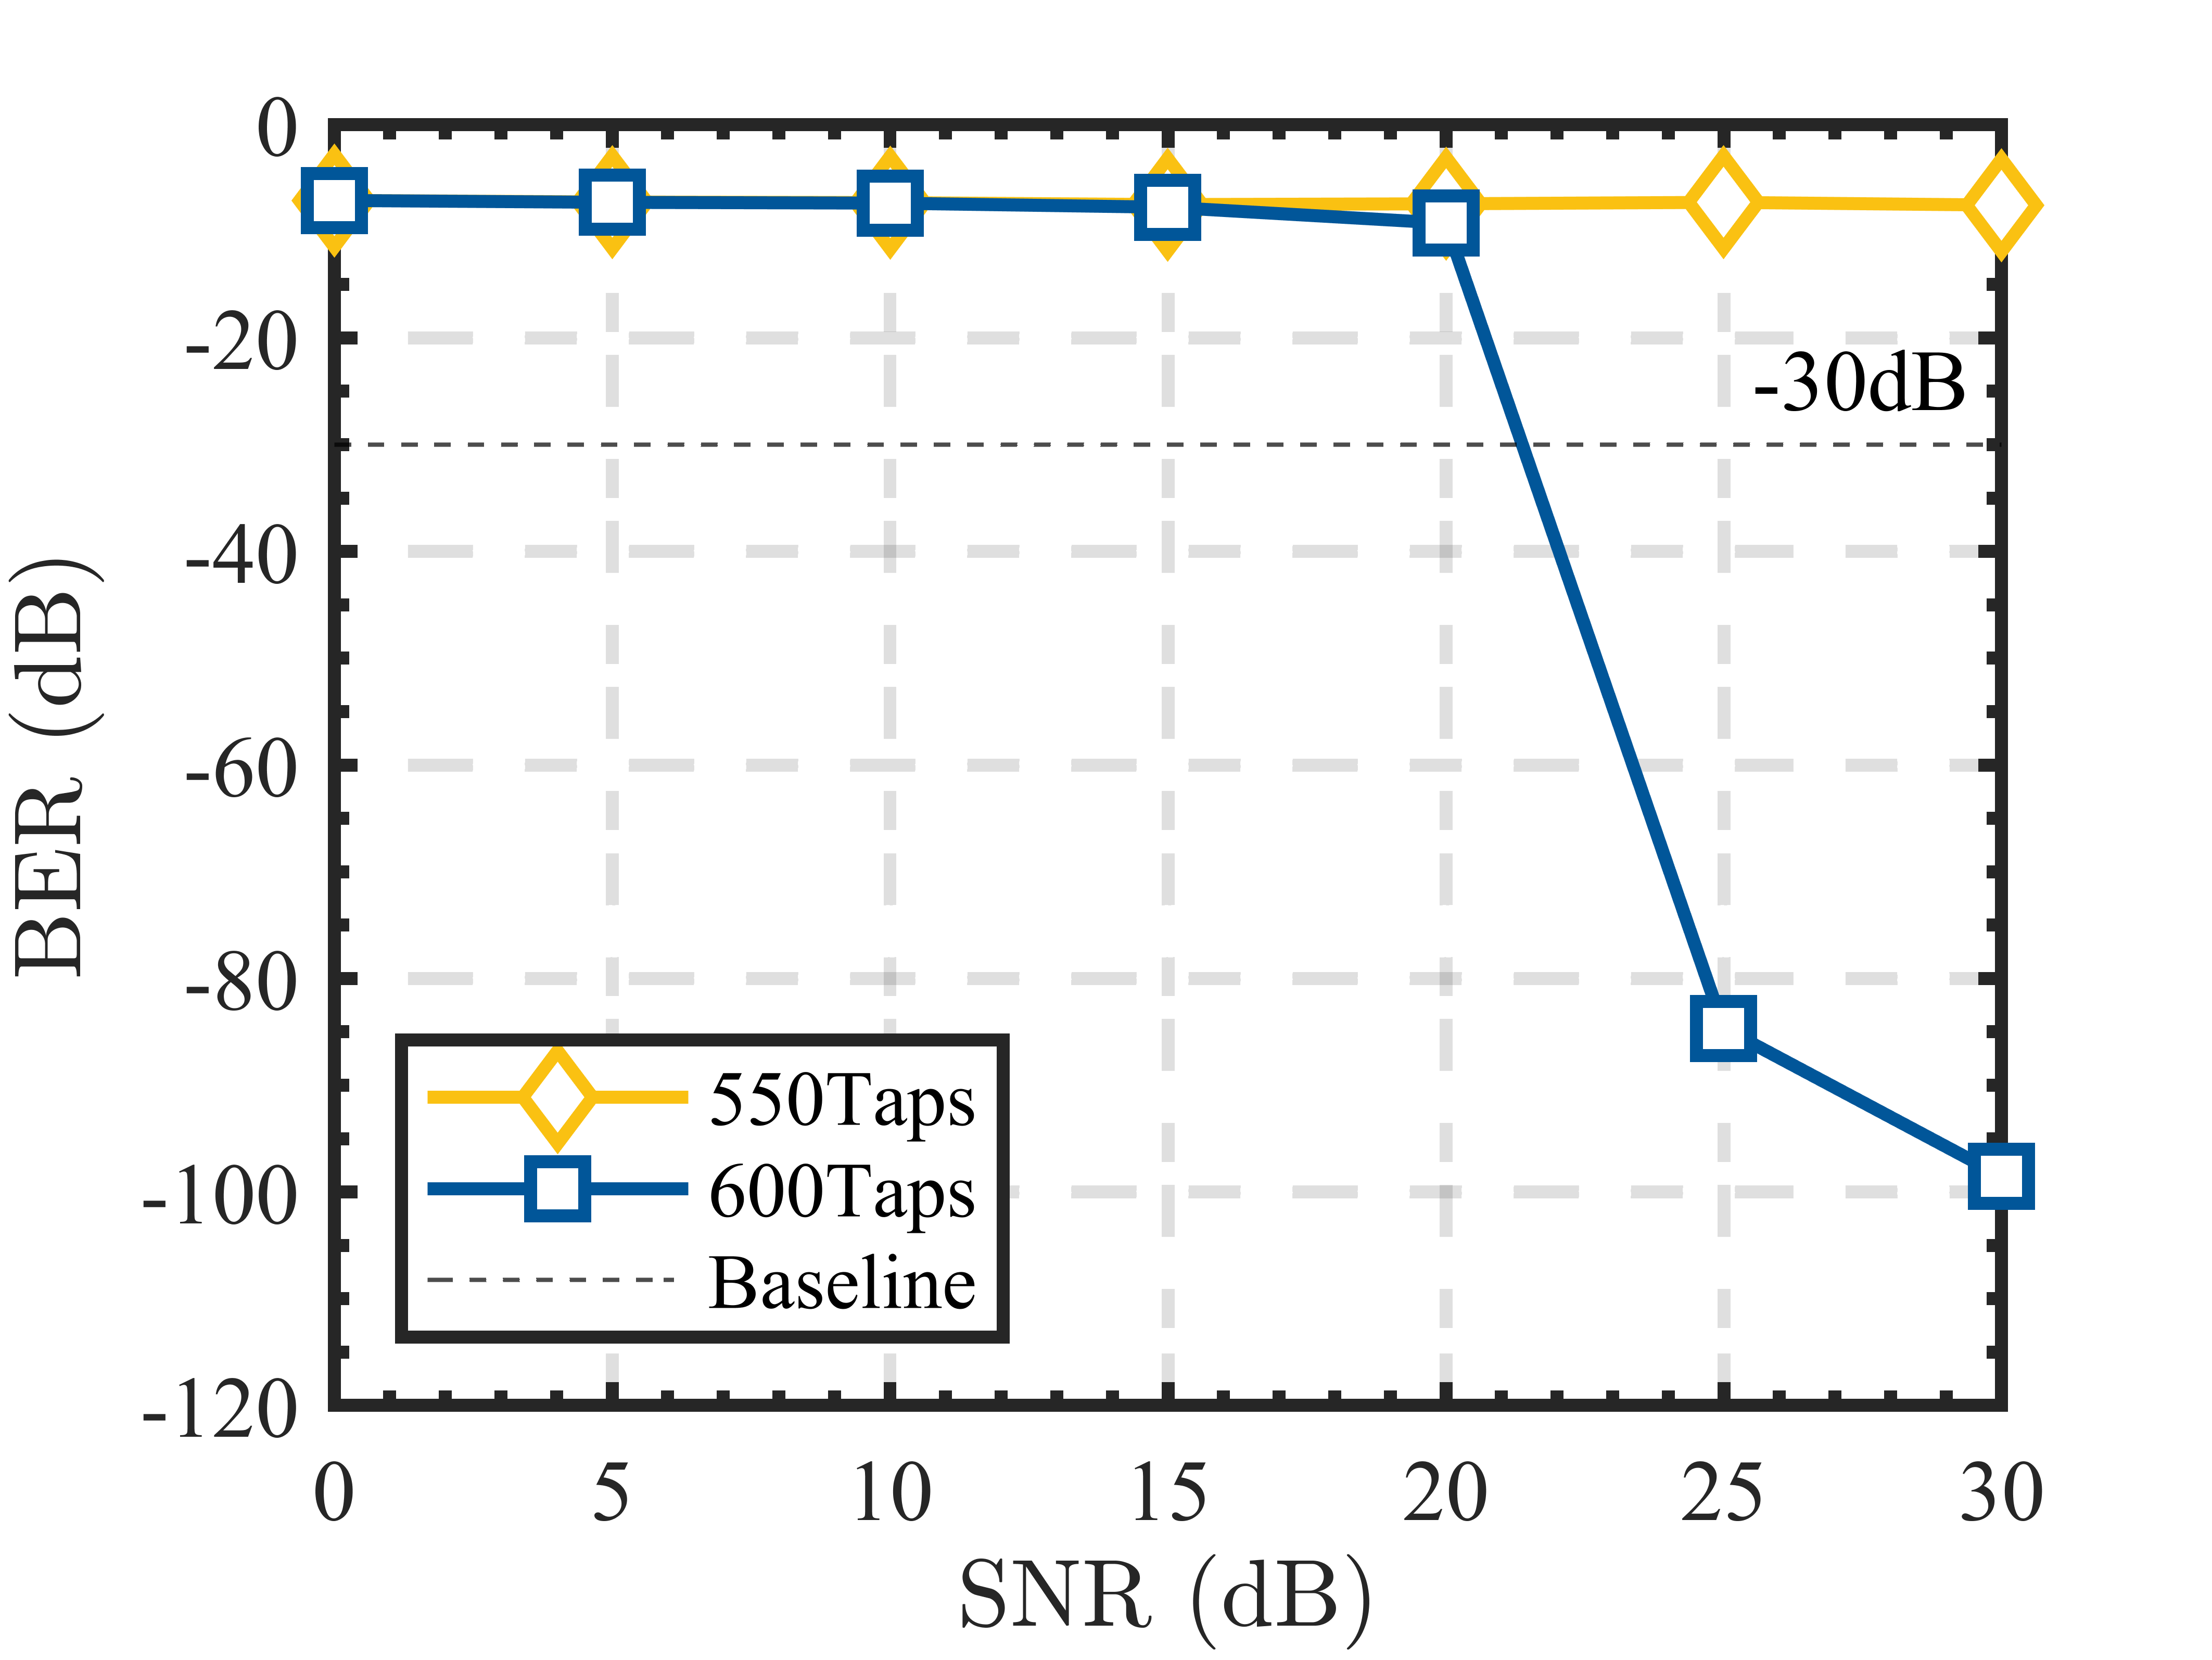
\includegraphics[width=2.5in]{fig/Taps_624.png}
\label{ber_taps_second}}
\\
\subfloat[]{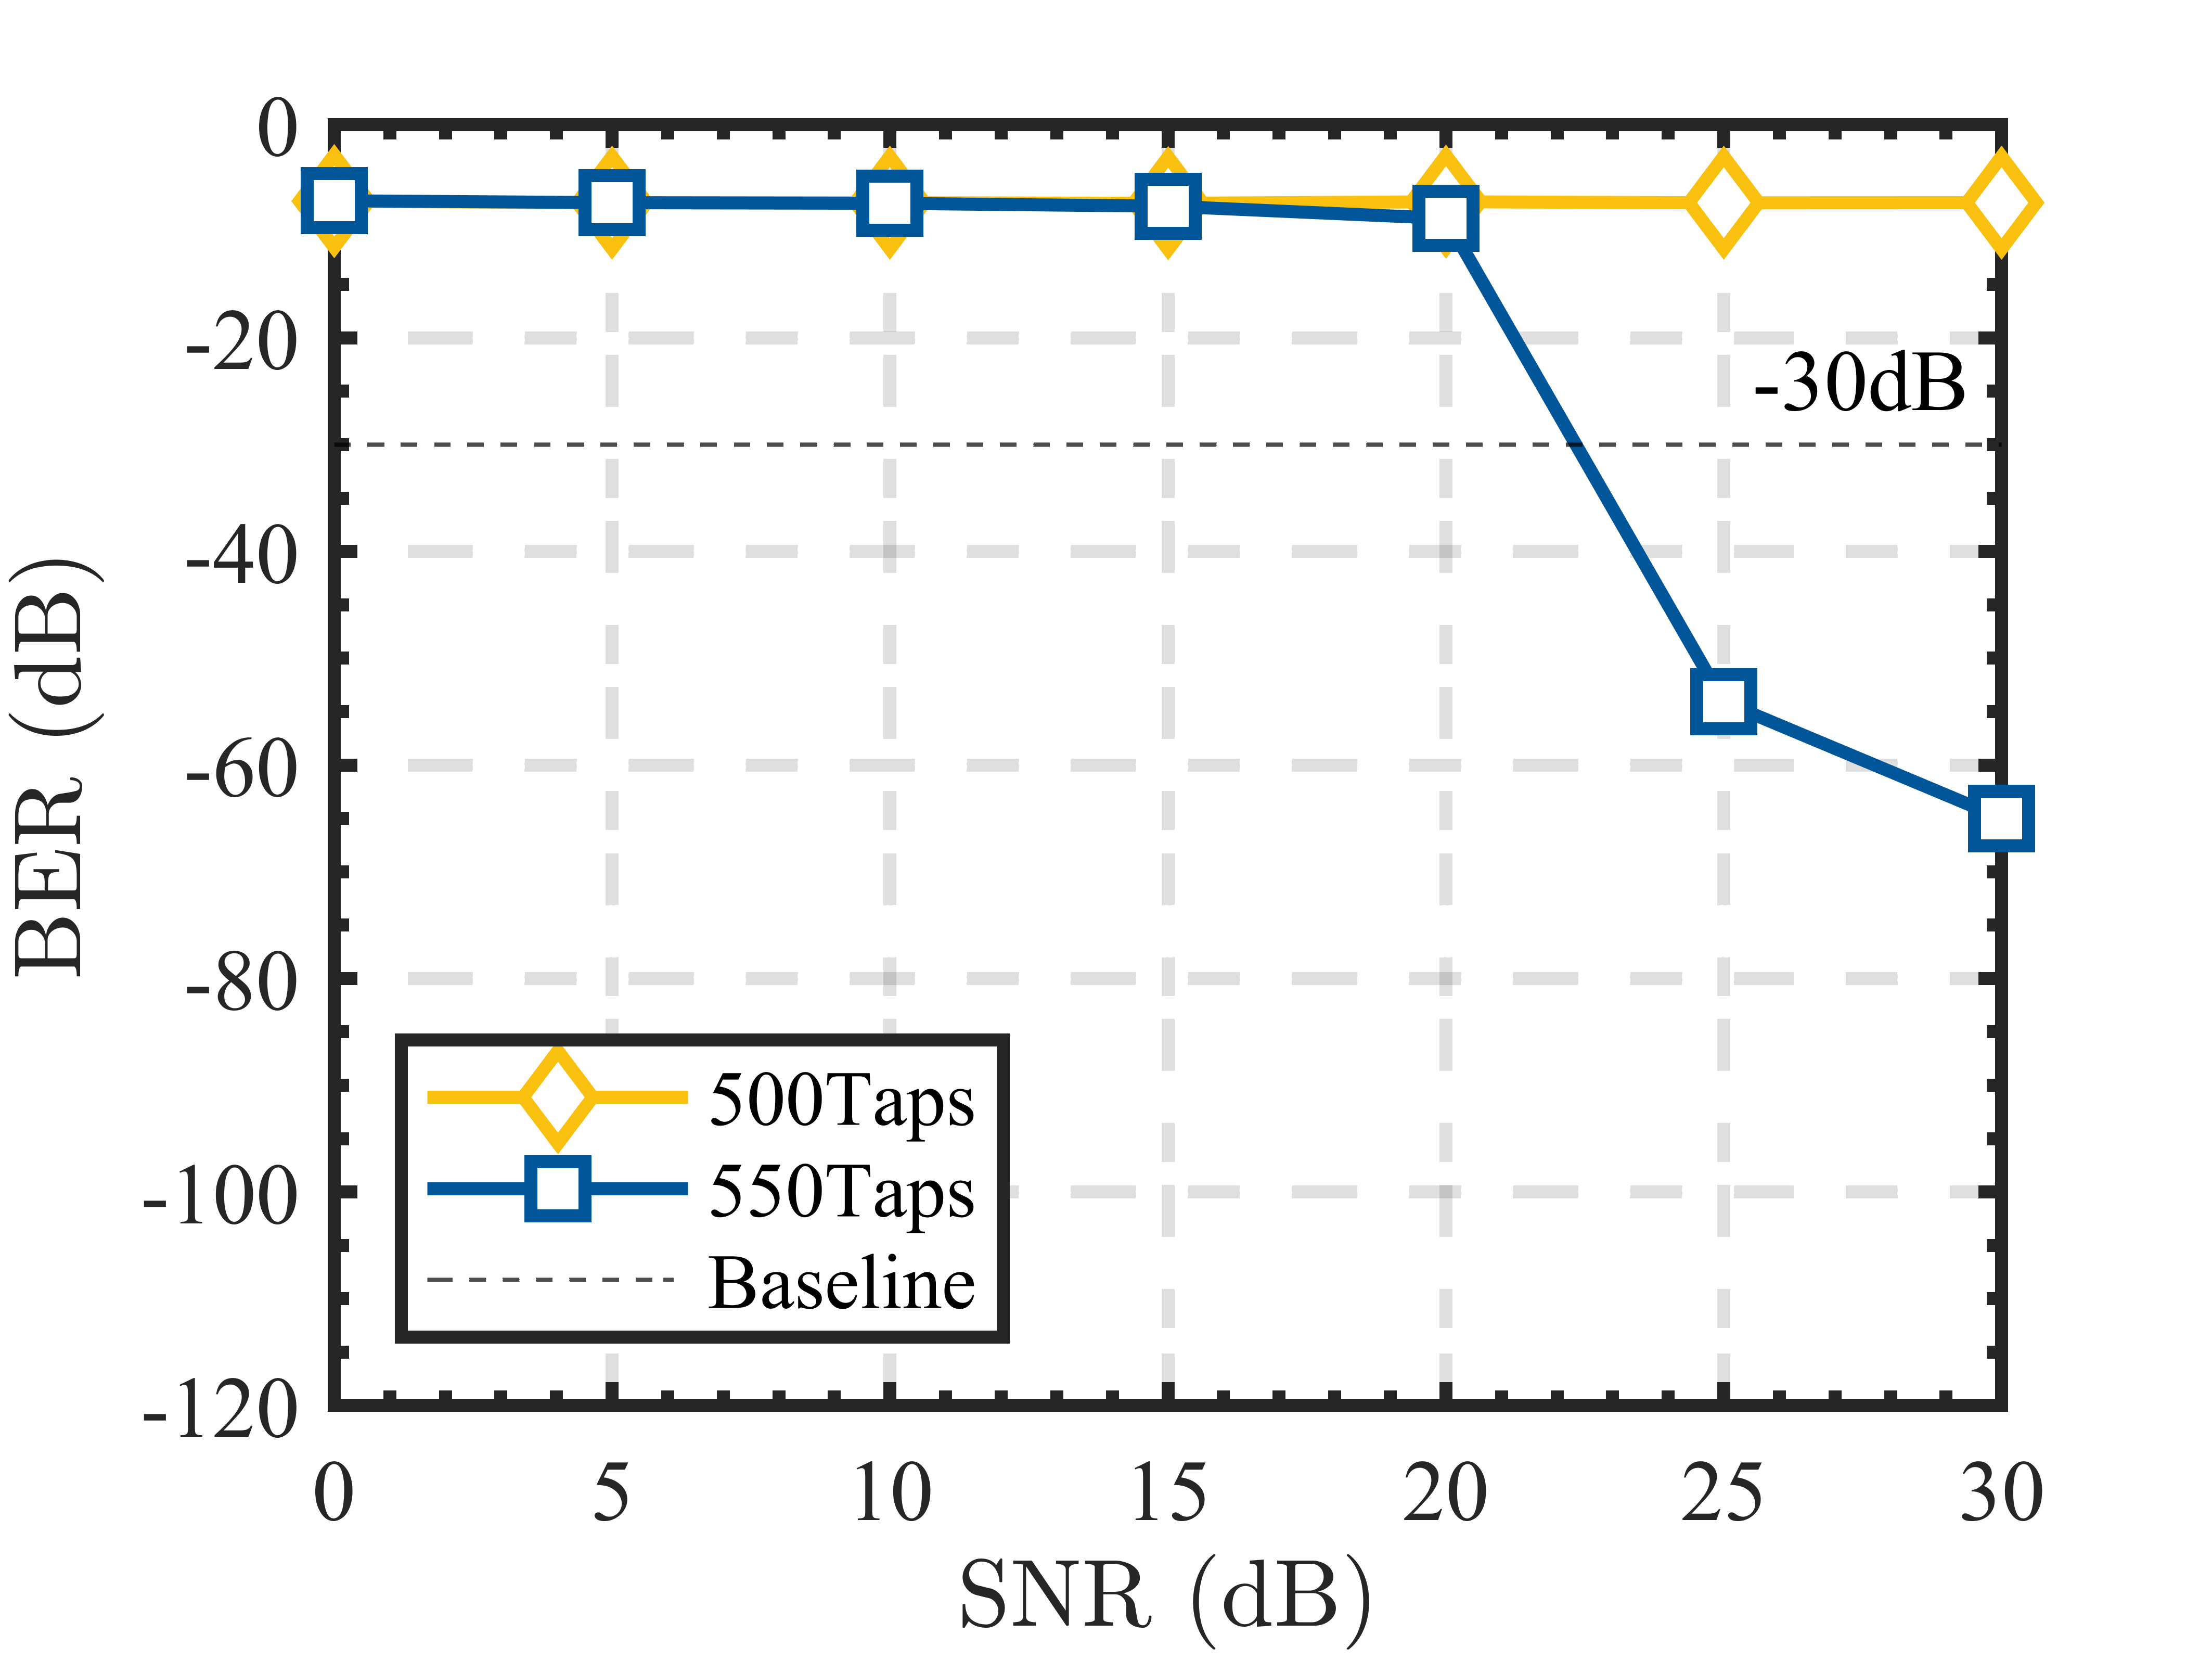
\includegraphics[width=2.5in]{fig/Taps_824.png}
\label{ber_taps_third}}
\hfil
\subfloat[]{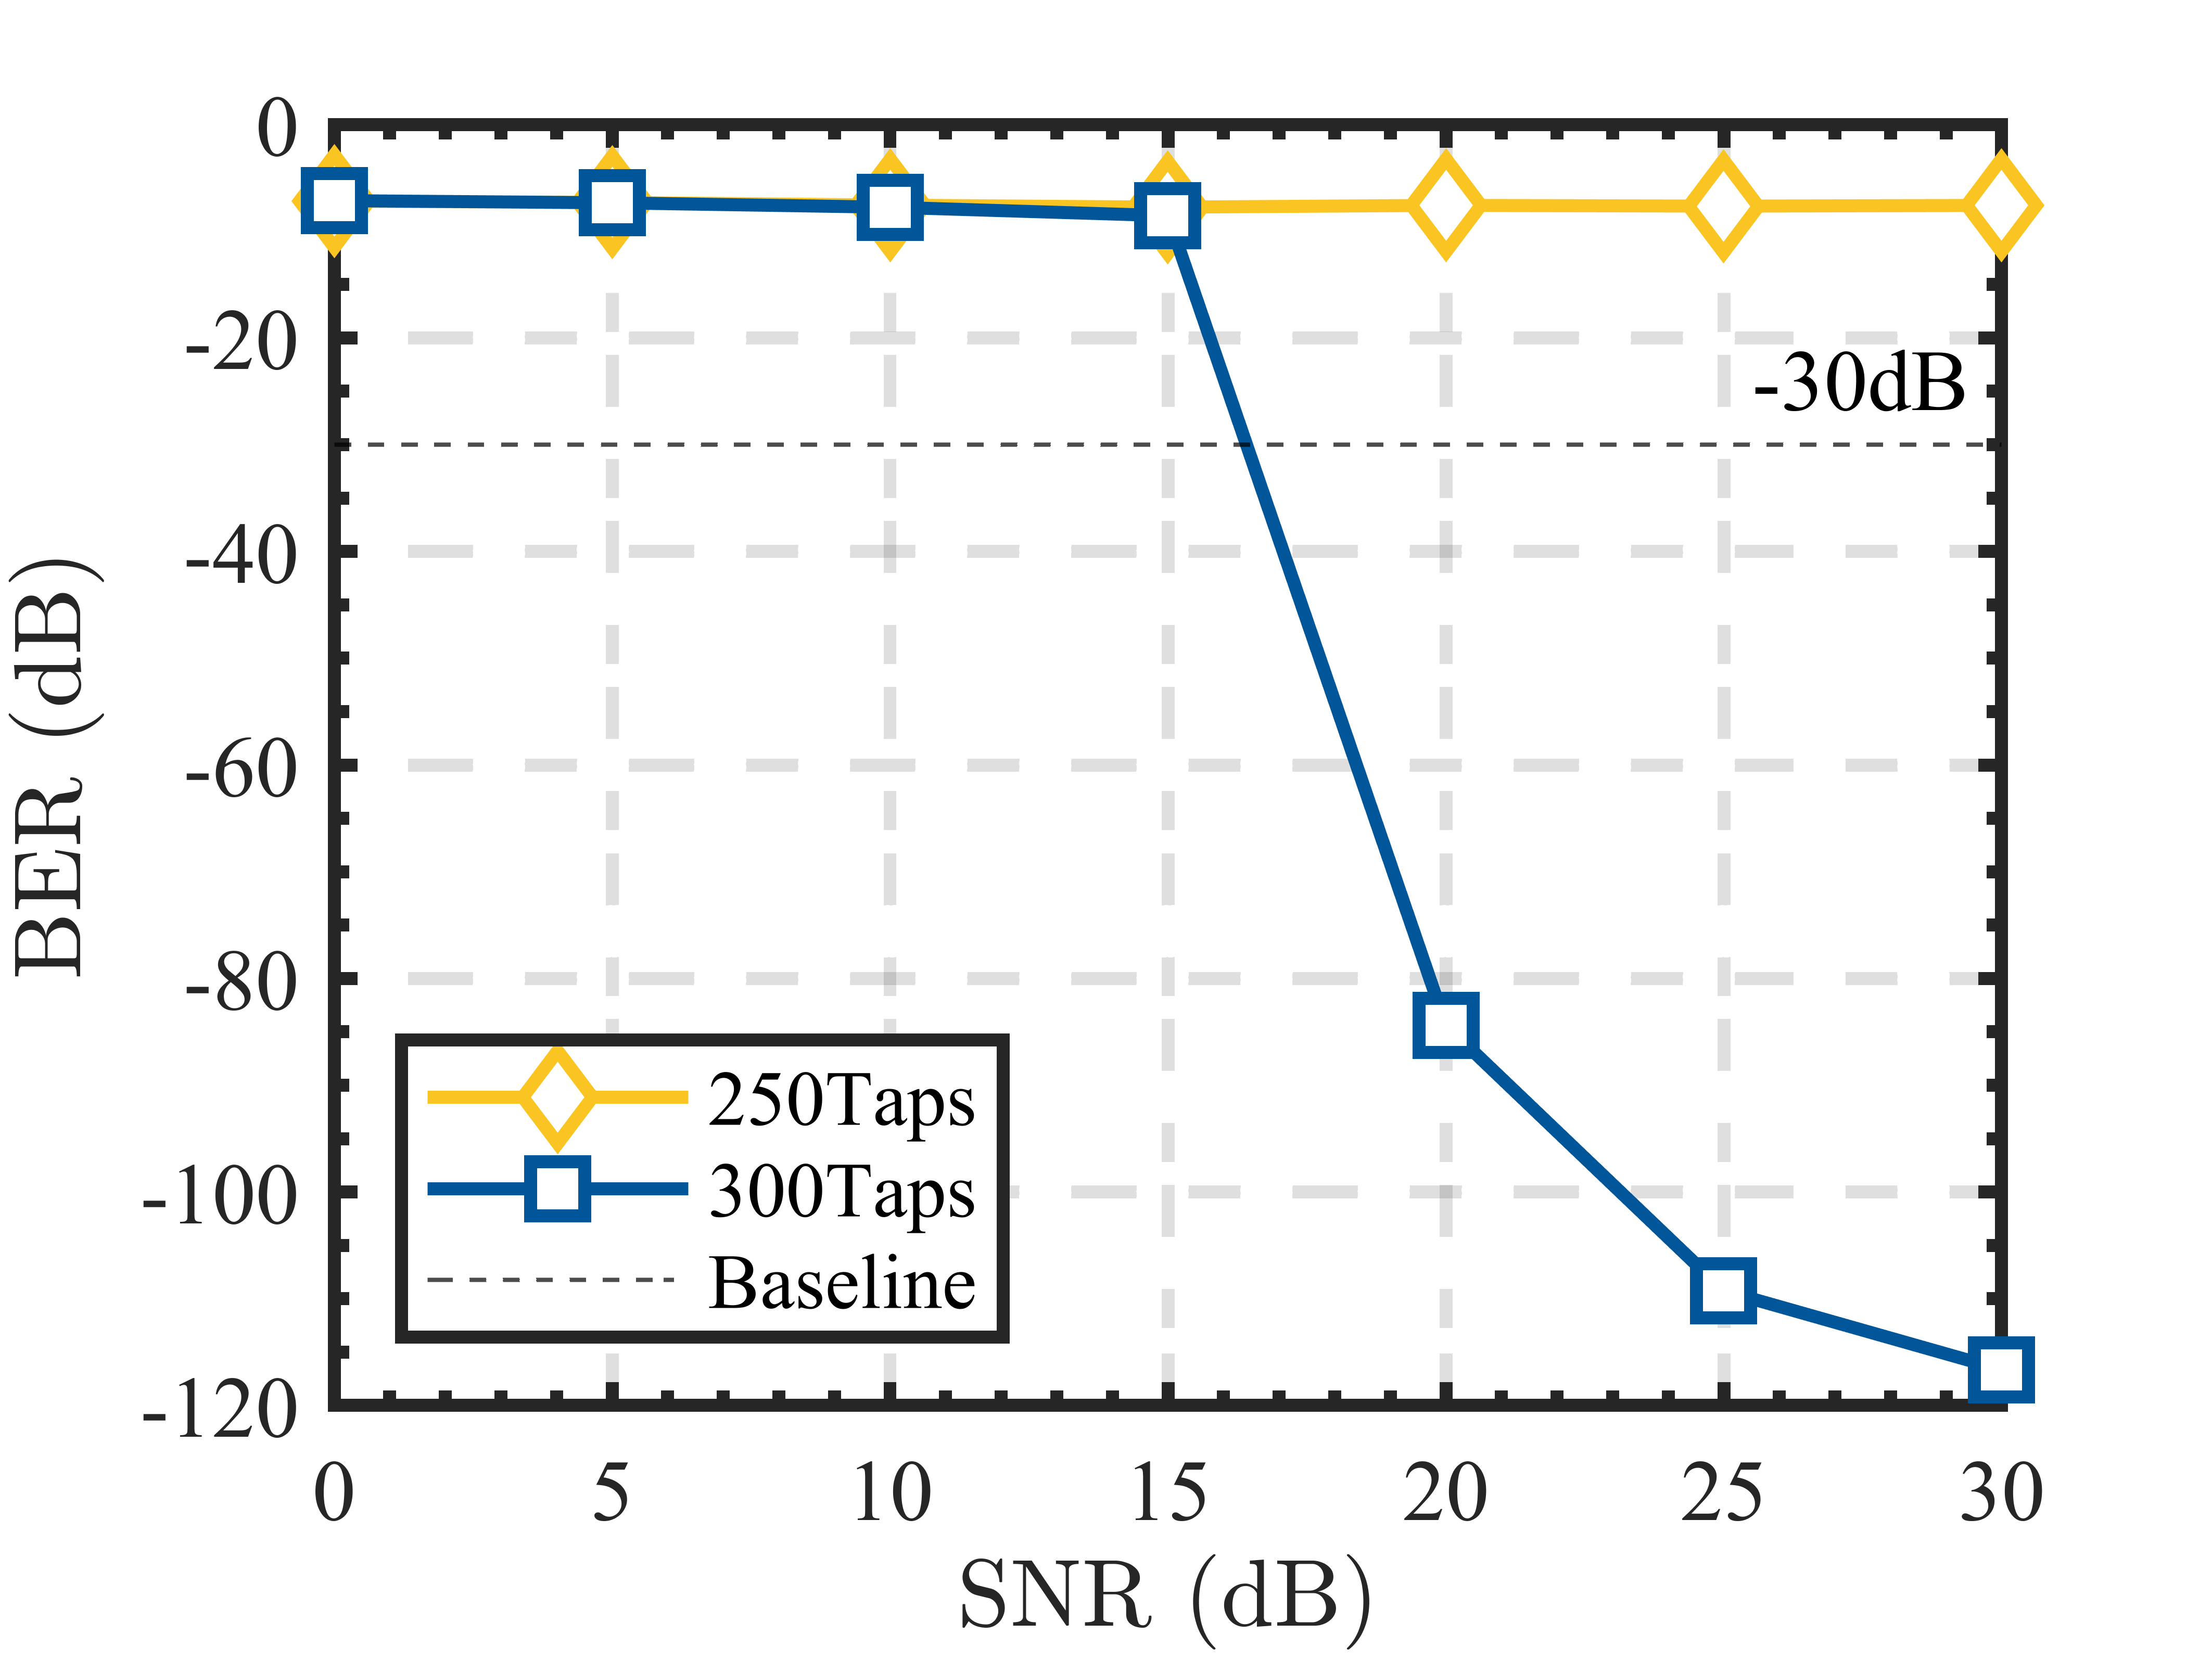
\includegraphics[width=2.5in]{fig/Taps_924.png}
\label{ber_taps_forth}}
\caption{Impact of the decision-feedback equalizer feedback filter length ($N_{\mathrm{fb}}$) on system performance at four depths: (a) 475.8~m, (b) 624.8~m, (c) 824.8~m, (d) 924.8~m.}
\label{fig:ber_taps}
\end{figure*}

The substantial depth-dependent variation in RMS delay spread, from 135.70~ms at 475.8~m to 160.30~ms at 824.8~m (Table~\ref{tab:channel_params}), has direct implications for receiver complexity. In single-carrier systems with decision-feedback equalization (DFE), the feedback filter must span the channel memory to suppress post-cursor ISI. Accordingly, the required feedback-filter length $N_{\mathrm{fb}}$ scales with normalized delay spread $\tau_{\mathrm{rms}}/T_s$, where $T_s$ is symbol duration.

To quantify this relationship, we conducted simulations using measured CIRs as channel realizations. While the original probe signals used BPSK to ensure robust channel estimation, the simulated link employs QPSK at 800 bps to evaluate realistic data transmission performance. A DFE updated by RLS adaptation is applied at the receiver. Fig.~\ref{fig:ber_taps} shows BER-versus-SNR performance for different $N_{\mathrm{fb}}$ values, with forgetting factor $\lambda$ optimized at each depth.

The results demonstrate striking depth-dependent requirements:
\begin{itemize}
    \item At 475.8~m, where $\tau_{\mathrm{rms}} = 135.70$~ms corresponds to approximately 54 symbol intervals, reliable communication ($\mathrm{BER} < 10^{-3}$) is achieved with $N_{\mathrm{fb}} = 90$ taps.
    \item At 824.8~m, where $\tau_{\mathrm{rms}}$ peaks at 160.30~ms ($\sim$64 symbols), achieving comparable performance requires $N_{\mathrm{fb}} \geq 550$ taps, a six-fold increase in computational complexity.
    \item The intermediate depths (624.8~m, 924.8~m) exhibit requirements commensurate with their respective delay spreads, requiring $N_{\mathrm{fb}} = 600$ and 300 taps, respectively.
\end{itemize}

In particular, insufficient $N_{\mathrm{fb}}$ produces error floors at all depths, but both floor severity and onset SNR vary strongly with depth. These results highlight a key design consideration: equalizer length should not be fixed a priori in deep sea systems and should be adapted to the operating depth.

\subsection{Implications for Tracking Algorithm Design: Coping with Time-Variation}
\label{subsec:tracking}

\begin{figure*}[!t]
\centering
\subfloat[]{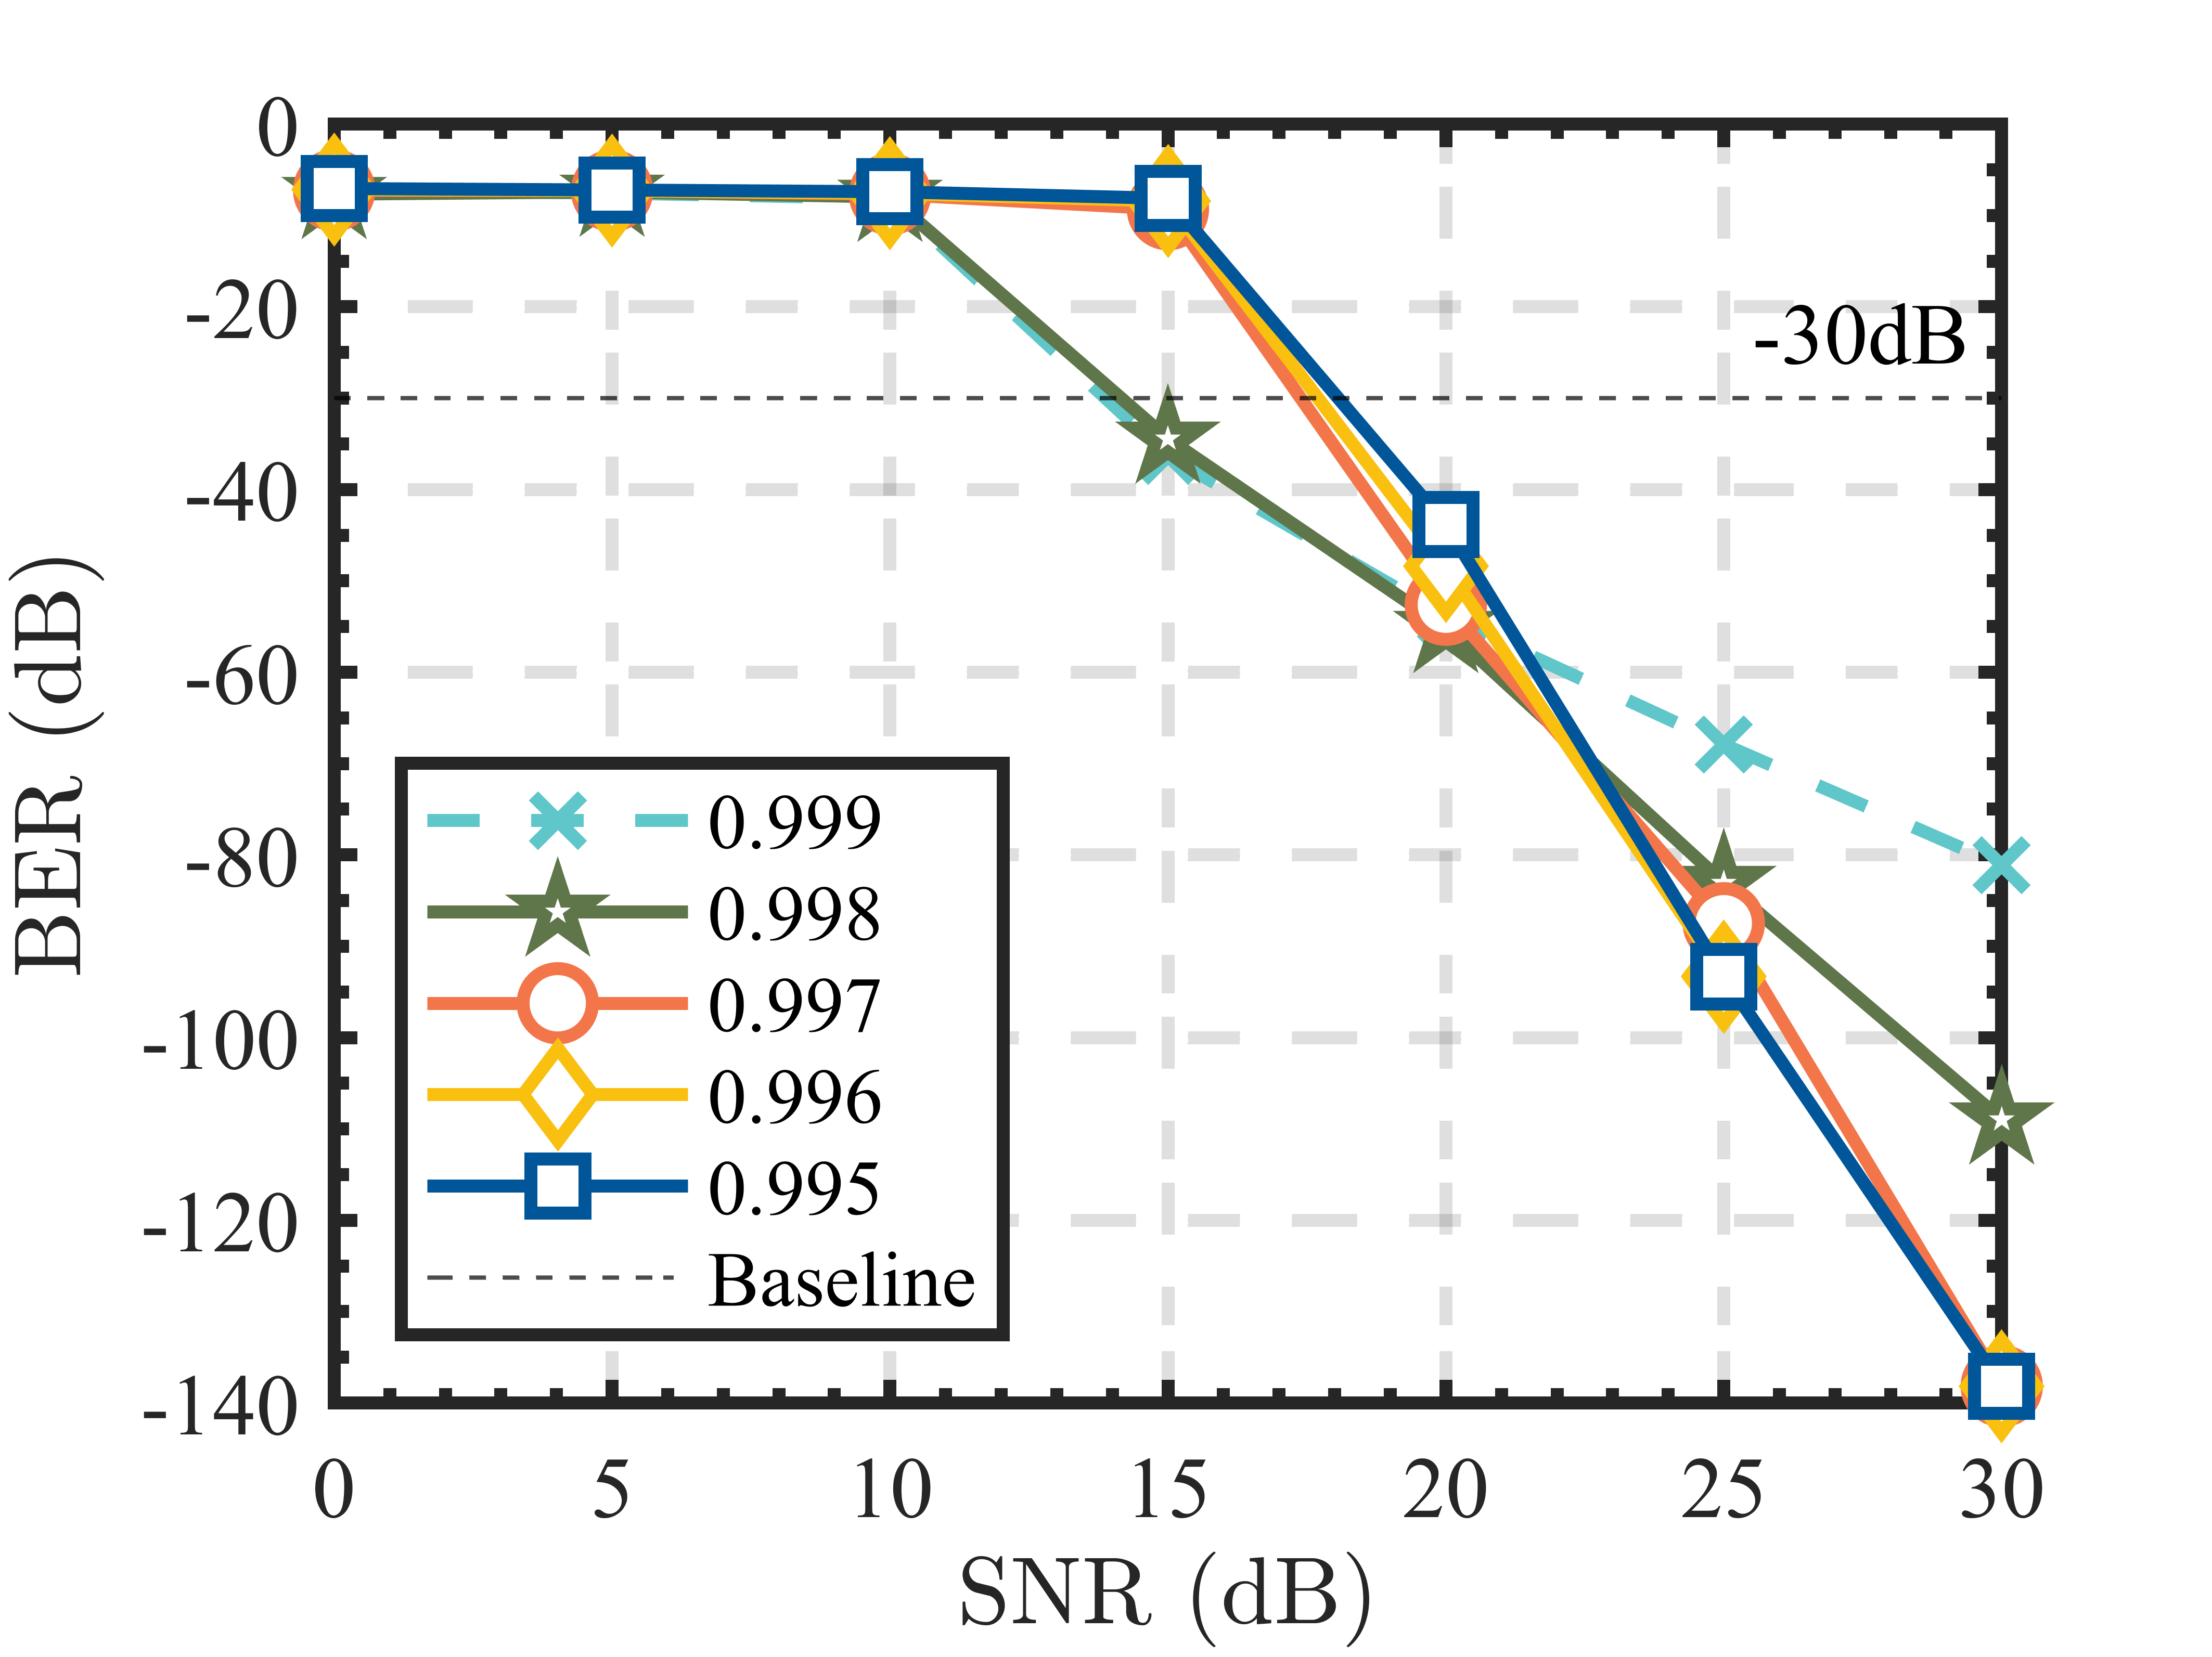
\includegraphics[width=2.5in]{fig/lambda_475.png}
\label{ber_lambda_first}}
\hfil
\subfloat[]{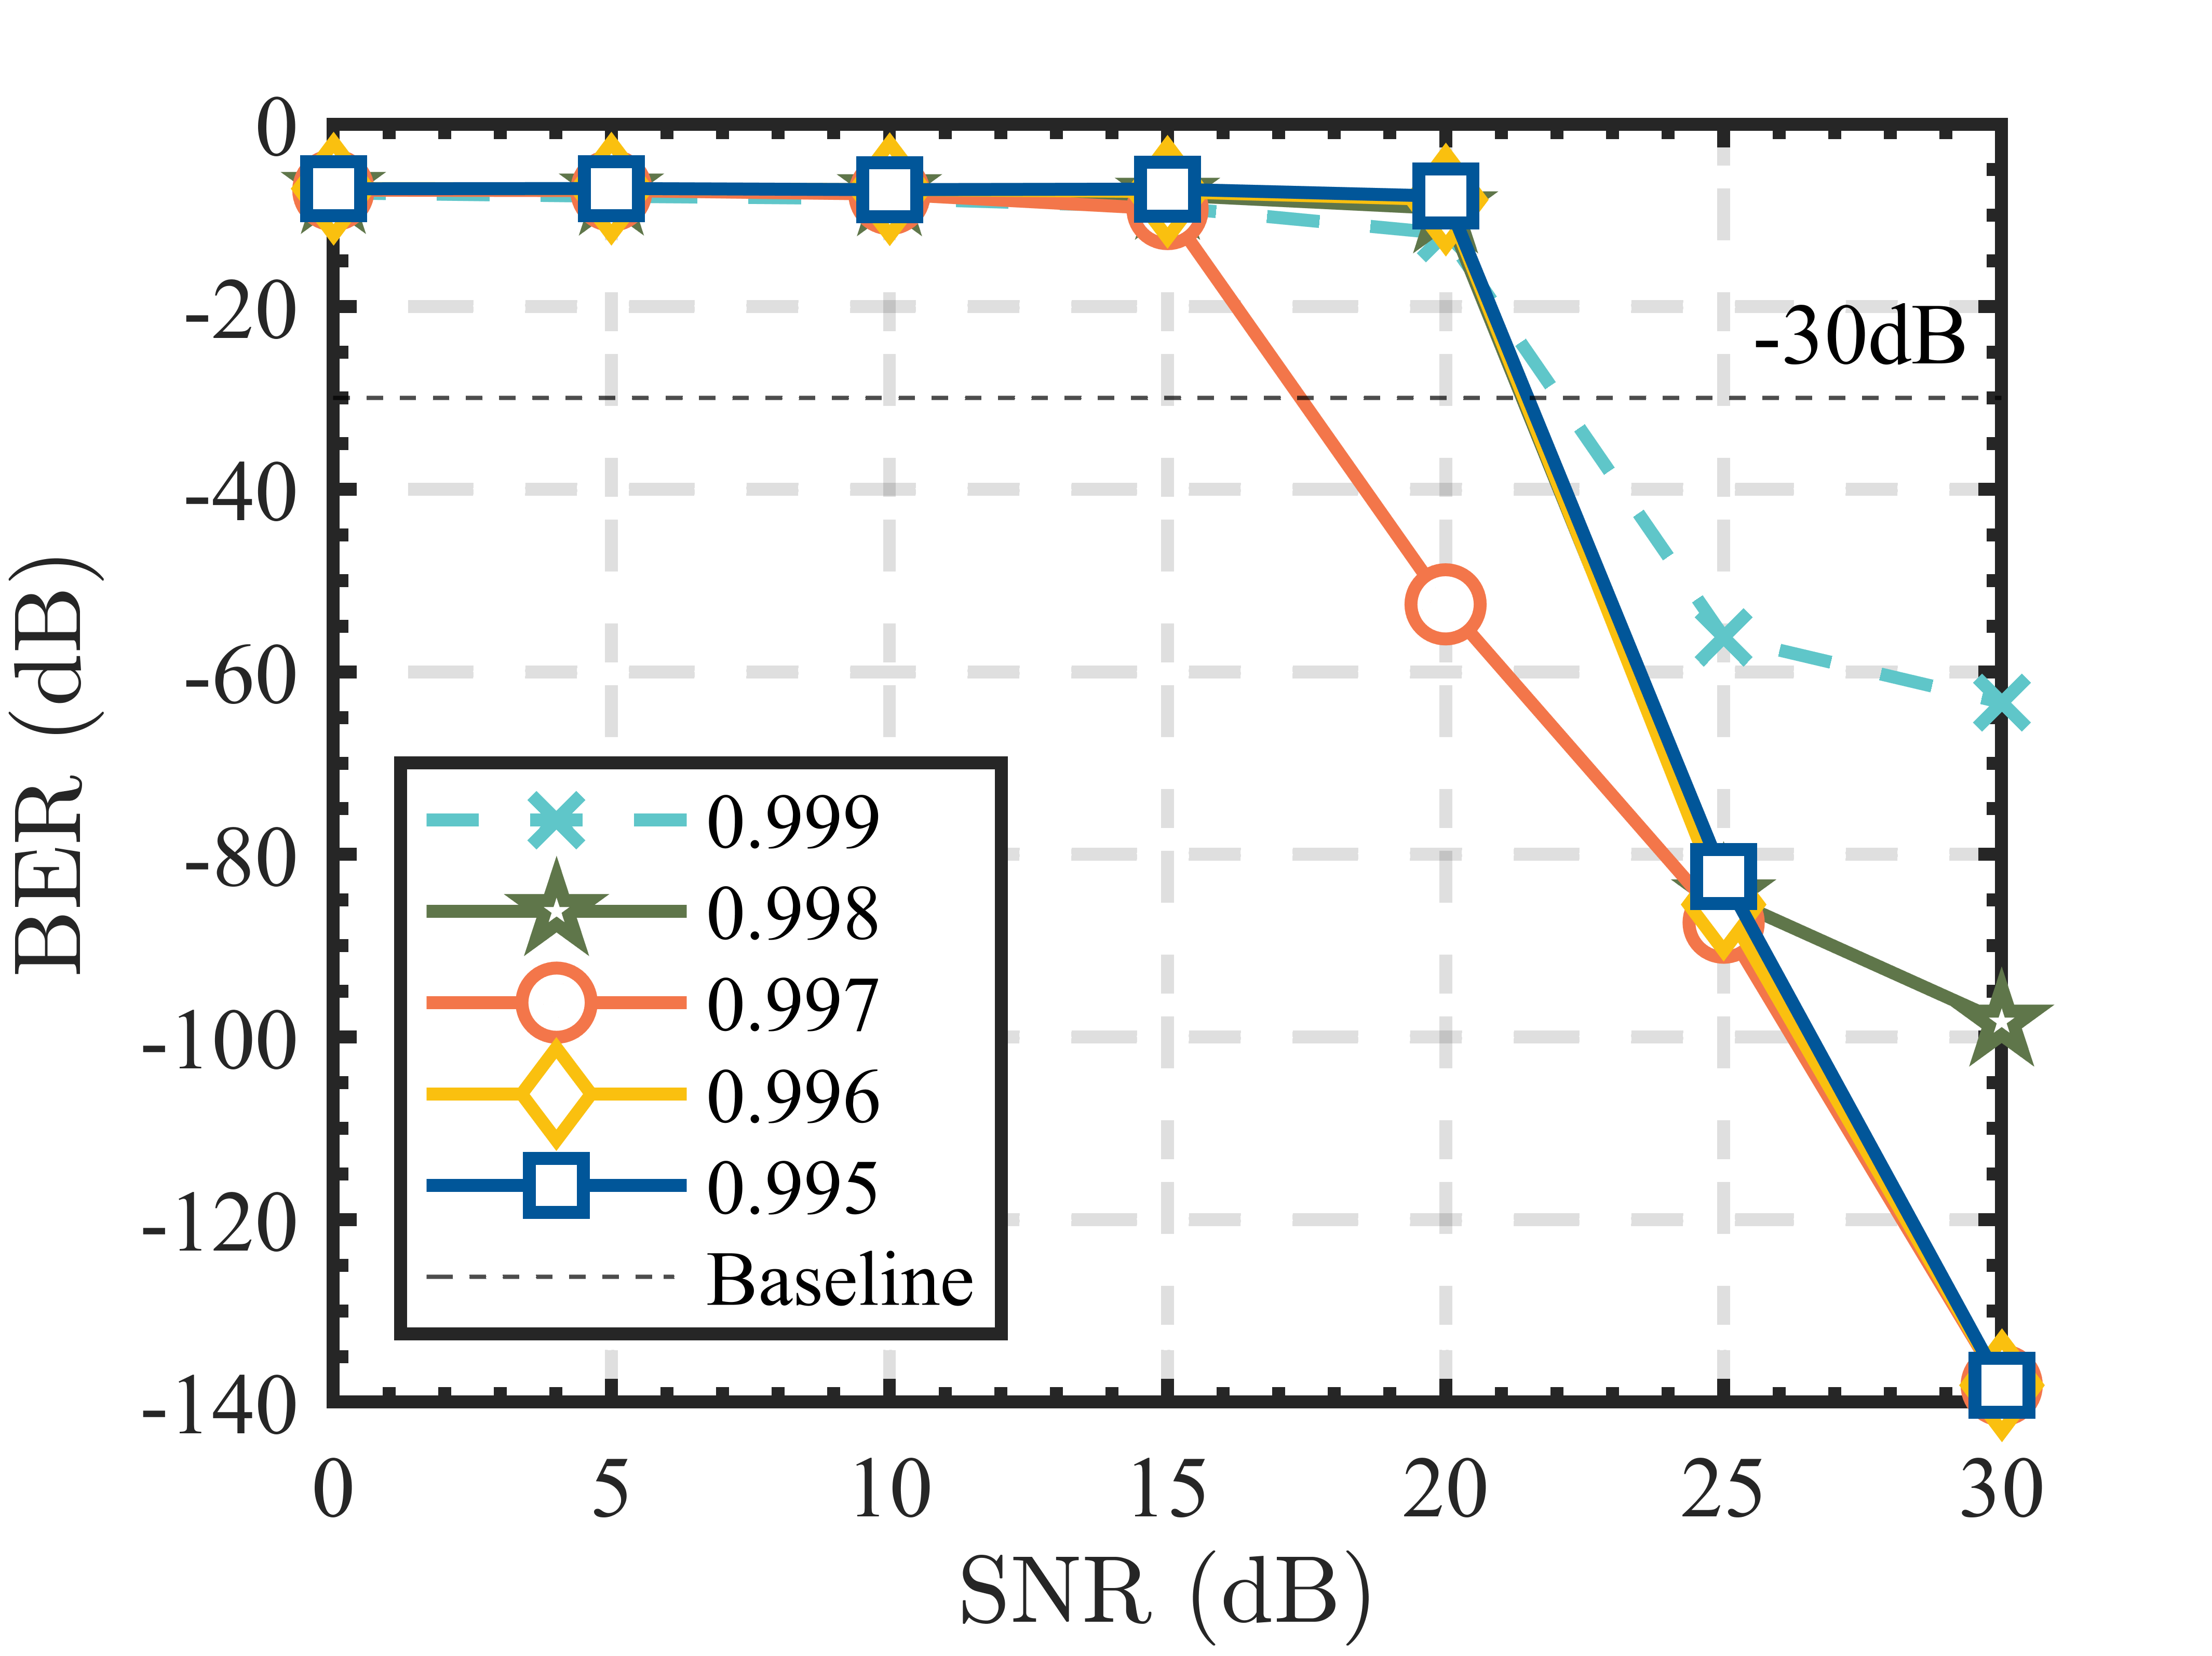
\includegraphics[width=2.5in]{fig/lambda_624.png}
\label{ber_lambda_second}}
\\
\subfloat[]{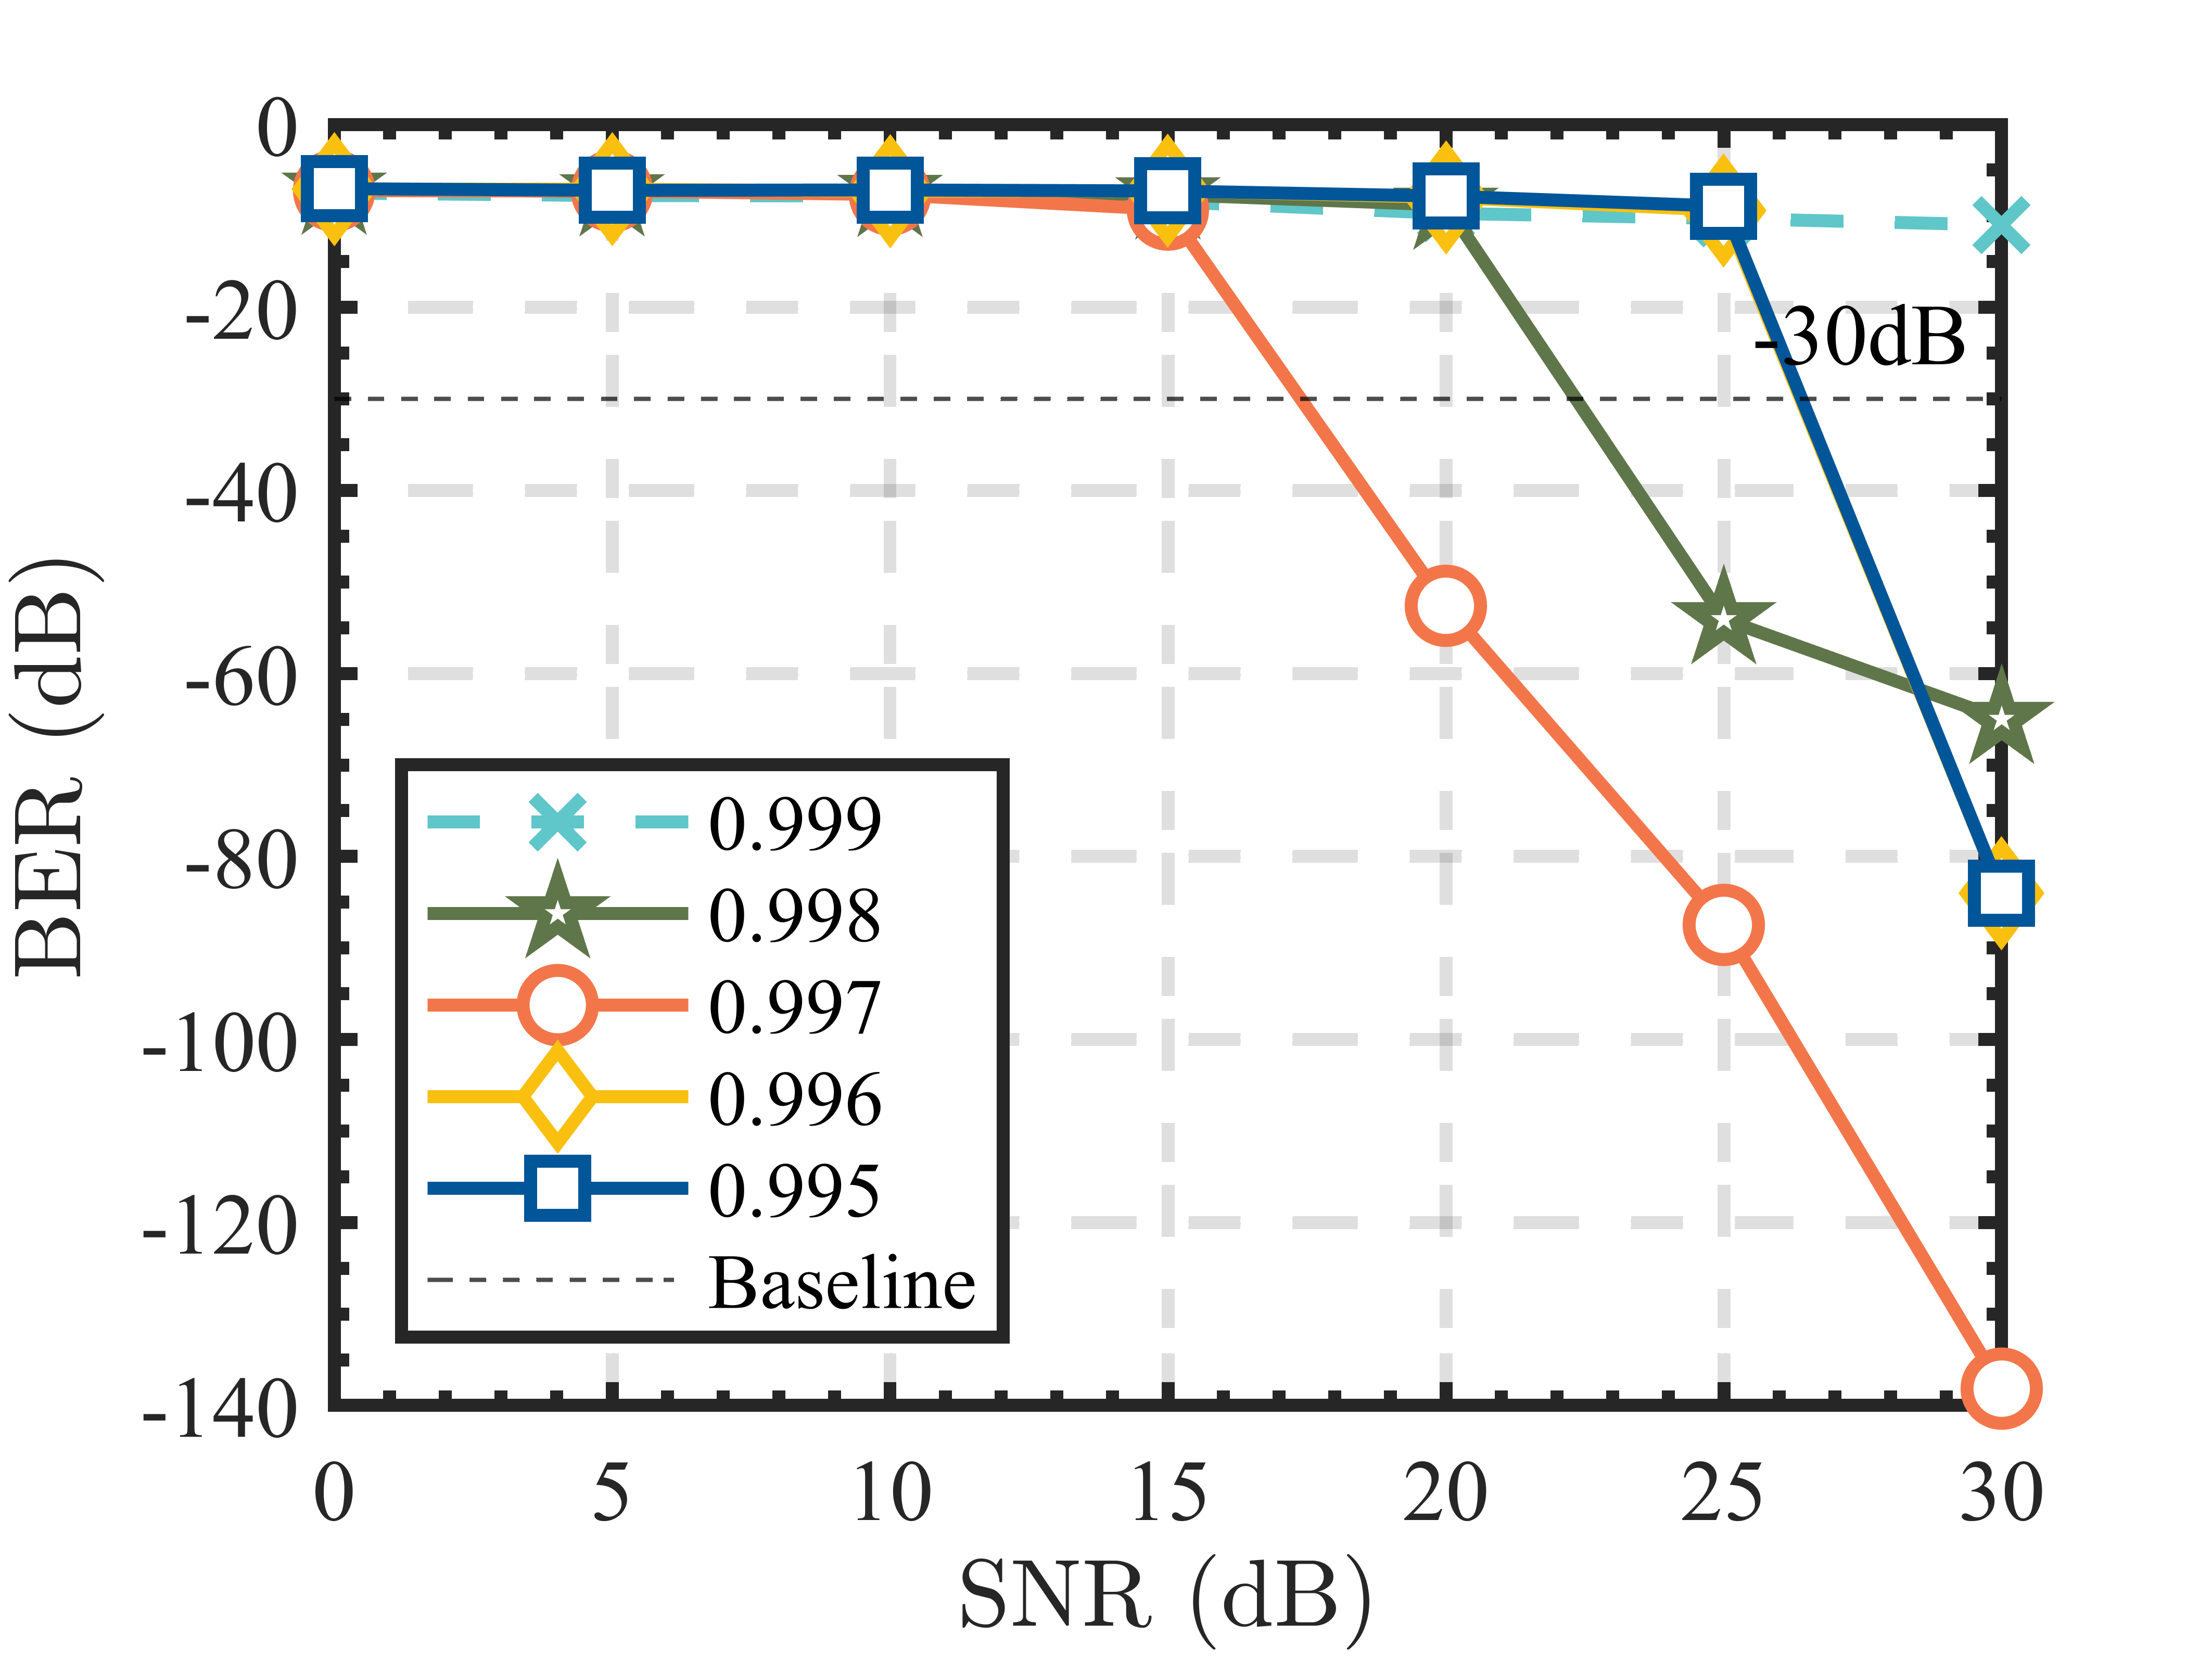
\includegraphics[width=2.5in]{fig/lambda_824.png}
\label{ber_lambda_third}}
\hfil
\subfloat[]{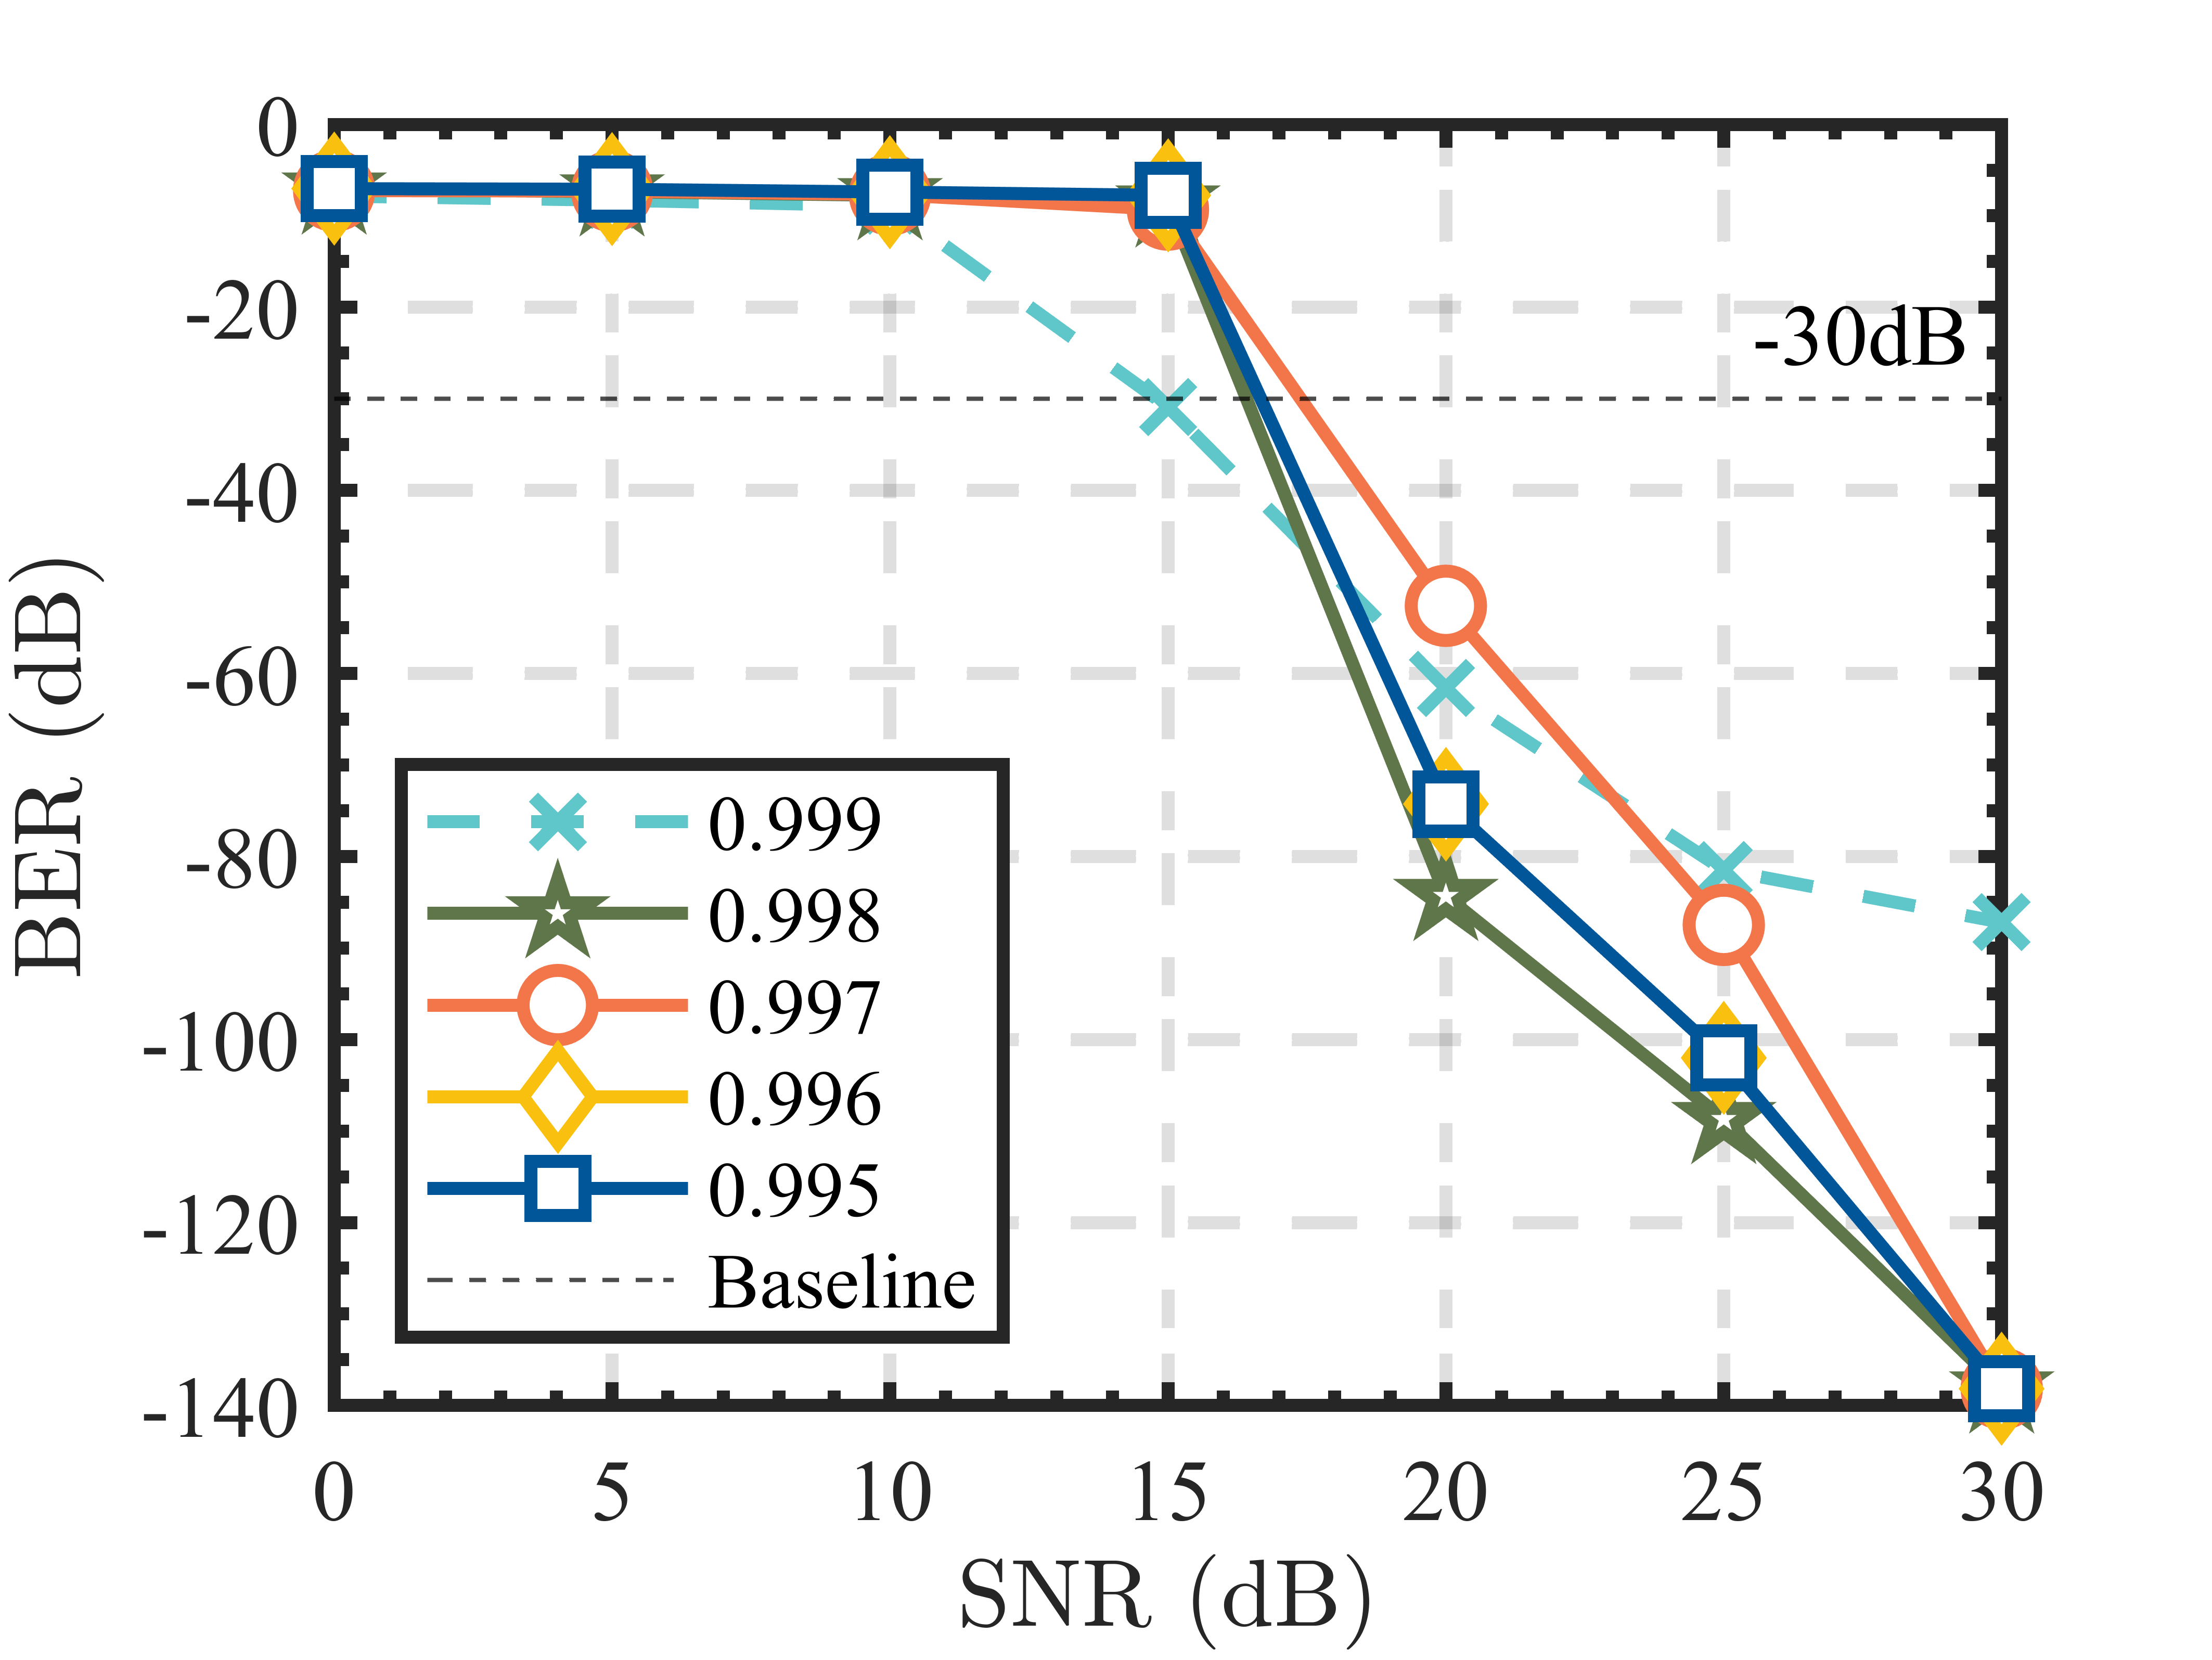
\includegraphics[width=2.5in]{fig/lambda_924.png}
\label{ber_lambda_forth}}
\caption{Impact of the RLS algorithm's forgetting factor ($\lambda$) on system performance at four depths: (a) 475.8~m, (b) 624.8~m, (c) 824.8~m, (d) 924.8~m.}
\label{fig:ber_lambda}
\end{figure*}

Although sufficient equalizer length mitigates multipath dispersion, robust communication over time-varying channels also requires adaptive tracking. In RLS, tracking behavior is governed by forgetting factor $\lambda \in (0,1]$, which sets the effective memory length $L_{\mathrm{eff}} = 1/(1-\lambda)$. Smaller $\lambda$ increases adaptation speed at the expense of higher steady-state misadjustment, whereas larger $\lambda$ improves noise robustness but risks lag under rapid channel variation.

Given the observed coherence-time variation, from 1003.09~ms at 475.8~m to 825.59~ms at 824.8~m, we hypothesized that the optimal $\lambda$ should decrease at depths with faster channel dynamics. Fig.~\ref{fig:ber_lambda} confirms this trend, showing BER-versus-SNR curves for different $\lambda$ values at each depth, with $N_{\mathrm{fb}}$ fixed to the minimum value that avoids severe ISI (from Fig.~\ref{fig:ber_taps}).



The optimal forgetting factors are:
\begin{itemize}
    \item $\lambda^* = 0.999$ for 475.8~m and 924.8~m (stable channels)
    \item $\lambda^* = 0.997$ for 624.8~m and 824.8~m (fast-varying channels)
\end{itemize}

This 0.002 decrease in $\lambda^*$ reduces effective memory from 1000 to 333 symbols, a three-fold reduction in the integration window needed to preserve tracking fidelity. The penalty for mismatched $\lambda$ is asymmetric: at high SNR, overly large $\lambda$ causes pronounced error floors because of tracking lag (notably at 824.8~m for $\lambda = 0.999$), while overly small $\lambda$ mainly degrades low-SNR performance through noise amplification.

Importantly, the depth dependence of the optimal $\lambda$ does not strictly track coherence-time ranking alone. Although 824.8~m has the shortest $T_c$, 624.8~m requires equally aggressive tracking. This indicates that multipath structure modulates sensitivity to temporal variation: at 824.8~m, dense energy-balanced multipath causes rapid fading even under moderate Doppler, while at 624.8~m, moderately complex multipath combined with shorter coherence yields similar tracking demand. Hence, both coherence time and multipath structure should guide tracking-parameter selection.

\subsection{Proposed DAVPR Architecture for AUVs}
\label{subsec:synthesis}

\begin{table*}[t]
\caption{Environment-Driven Lookup Table}
\label{tab:design_principles}
\centering
\begin{tabular}{|c|c|c|c|c|}
\hline
\textbf{Depth Range} & \textbf{Dominant Characteristic} & \textbf{$N_{\mathrm{fb}}$} & \textbf{$\lambda^*$} & \textbf{Primary Consideration} \\
\hline
Upper main  thermocline  (450-- 600~m)& Moderate delay, weak time-variation & 90--150 & 0.999 & Computational efficiency \\
\hline
Lower main thermocline (600--900~m)& Peak delay spread, strong time-variation & 500--600 & 0.997 & Robustness to ISI and fading \\
\hline
Main thermocline base  ($>$ 900~m)& Reduced delay, moderate time-variation & 250--350 & 0.999 & Balance of complexity and stability \\
\hline
\end{tabular}
\end{table*}


Taken together, Figs.~\ref{fig:ber_taps} and \ref{fig:ber_lambda} demonstrate that optimal deep sea communication performance cannot be achieved with a static receiver configuration. To translate these physical-layer insights into a practical, energy-efficient system, we propose the DAVPR architecture tailored for AUVs. Rather than maintaining a fixed maximum-complexity structure or relying on continuous, computation-heavy channel estimation, DAVPR adaptively scales its equalizer length ($N_{fb}$) and tuning parameters ($\lambda$) based on the node's real-time vertical position.

The core of the DAVPR framework is an Environment-Driven Lookup Table, formalized in Table~\ref{tab:design_principles}. This table directly maps specific thermocline strata to their corresponding optimal receiver configurations. This design leverages a crucial hardware energy trade-off: in practical AUV deployments, digital signal processors (DSPs) performing continuous full-channel estimation and maximum-length filtering consume substantial power (typically in the Watt range). By contrast, onboard depth/pressure sensors consume negligible power (in the milliwatt range). Using low-power pressure telemetry to dynamically govern DSP complexity represents a highly efficient energy-performance trade-off.

To deploy the DAVPR architecture in real-world scenarios, we propose three implementation strategies that exploit the observed thermocline stratification:
\begin{enumerate}
    \item \textit{Mission-preplanned adaptation}: Using offline parameter scheduling based on the AUV's pre-programmed depth-time waypoints.
    \item \textit{Real-time pressure-sensing with lookup tables}: Continuously matching the AUV's real-time depth telemetry against the environment-driven lookup table (Table~\ref{tab:design_principles}) to trigger structural scaling.
    \item \textit{Hybrid initialization}: Using the node's position within the thermocline to provide coarse parameter bounds, which are subsequently refined by low-overhead pilot-aided tracking.
\end{enumerate}

Among these, approach (2) is particularly effective for autonomous platforms. Since the regional sound-speed profile is typically known \textit{a priori} or changes slowly, real-time pressure measurements unambiguously map to specific thermocline segments. This physics-guided strategy allows DAVPR to effectively bypass the computationally expensive full-channel estimation traditionally required for initial receiver configuration. By preventing over-equalization in shallow layers and preventing tracking lag in deep convergence zones, this depth-to-parameter mapping serves as an essential, robust, and resource-saving solution for deep sea AUV communications.

\section{Conclusion}
\label{sec:conclusion}

This paper investigated acoustic channel characteristics across the main thermocline using experimental data from the South China Sea. Our analysis reveals regime-dependent stratification that defies simple depth-scaling: the lower thermocline convergence zone exhibits peak multipath complexity and reduced temporal coherence, while the upper thermocline and thermocline base present contrasting propagation conditions. These findings challenge the conventional assumption of monotonic deep-water stability and demonstrate that classical channel relationships break down across thermocline regimes.

System-level simulations confirm that receiver parameters are more effective when they are thermocline-adaptive rather than uniformly depth-scaled: equalizer length needs to be expanded in the lower thermocline convergence zone to mitigate severe inter-symbol interference from refractive multipath focusing, while adaptation rates should be regime-matched—faster tracking in the lower thermocline for rapid decorrelation, relaxed adaptation in the upper thermocline for computational efficiency, and moderate settings at the thermocline base for stable deep-water conditions.

These findings provide essential physical-layer insights for designing a DAVPR architecture for robust deep sea communication. Future work will validate these regime-specific trends in diverse hydrological environments and develop autonomous protocols that adjust physical-layer parameters based on real-time thermocline regime identification.

% \section*{Acknowledgments}
% The authors thank the sea-trial team and supporting institutions for their assistance in experiment deployment, data collection, and logistics.



% {\appendix[Proof of the Zonklar Equations]
% Use $\backslash${\tt{appendix}} if you have a single appendix:
% Do not use $\backslash${\tt{section}} anymore after $\backslash${\tt{appendix}}, only $\backslash${\tt{section*}}.
% If you have multiple appendixes use $\backslash${\tt{appendices}} then use $\backslash${\tt{section}} to start each appendix.
% You must declare a $\backslash${\tt{section}} before using any $\backslash${\tt{subsection}} or using $\backslash${\tt{label}} ($\backslash${\tt{appendices}} by itself
%  starts a section numbered zero.)}



%{\appendices
%\section*{Proof of the First Zonklar Equation}
%Appendix one text goes here.
% You can choose not to have a title for an appendix if you want by leaving the argument blank
%\section*{Proof of the Second Zonklar Equation}
%Appendix two text goes here.}


%\begin{thebibliography}{1}
%\bibliographystyle{IEEEtran}
%\end{thebibliography}

\begin{thebibliography}{22}
\bibliographystyle{IEEEtran}

\bibitem{ref1}
J. Cui, G. Han, Y. Su, and X. Fu, ``Non-uniform non-orthogonal multicarrier underwater communication for compressed sonar image data transmission,'' \textit{IEEE Trans. Veh. Technol.}, vol. 70, no. 10, pp. 10133--10145, Oct. 2021.

\bibitem{ref2}
X. Wang, J. Liu, G. Han, J. Wang, and J. Cui, ``End-to-end modulation recognition in underwater acoustic communications using temporal large kernel convolution with gated channel mixer,'' \textit{IEEE Trans. Veh. Technol.}, vol. 73, no. 10, pp. 15076--15086, Oct. 2024.

\bibitem{ref3}
Q. Meng, J. Huang, J. Han, C. He, and C. Ma, ``An improved direct adaptive multichannel turbo equalization scheme for underwater communications,'' in \textit{OCEANS 2012 - Yeosu}, Yeosu, South Korea, May 2012.

\bibitem{ref4}
Z. Yang, T. Liang, Z. Deng, and Y. Zhang, ``Improved proportionate FONLMS algorithm based direct adaptive turbo equalization for MIMO underwater acoustic communications,'' in \textit{2nd Franco-Chinese Acoustic Conference (FCAC 2018)}, Le Mans, France, Oct. 2018, vol. 283, \textit{MATEC Web of Conferences}.

\bibitem{ref5}
D. Li, Y. Wu, M. Zhu, and X. Wu, ``Efficient faster-than-nyquist transceiver design for underwater acoustic communications,'' in \textit{Proc. Int. Conf. Underwater Netw. Syst. (WUWNET)}, Atlanta, GA, USA, Oct. 2019.

\bibitem{ref6}
H. Zhao, C. Yang, Y. Xu, F. Ji, M. Wen, and Y. Chen, ``Model-driven based deep unfolding equalizer for underwater acoustic ofdm communications,'' \textit{IEEE Trans. Veh. Technol.}, vol. 72, no. 5, pp. 6056--6067, May 2023.

\bibitem{ref7}
J. Huang and R. Diamant, ``Adaptive modulation for long range underwater acoustic communication,'' \textit{IEEE Trans. Wireless Commun.}, vol. 19, no. 10, pp. 6844--6857, Oct. 2020.

\bibitem{ref8}
Q. Fu and A. Song, ``Adaptive modulation for underwater acoustic communications based on reinforcement learning,'' in \textit{OCEANS 2018 MTS/IEEE Charleston}, Charleston, SC, USA, Oct. 2018.

\bibitem{ref9}
M. Stojanovic and L. Freitag, ``Wideband underwater acoustic CDMA: Adaptive multichannel receiver design,'' in \textit{OCEANS 2005}, Washington, DC, USA, Sep. 2005, pp. 1508--1513.

\bibitem{ref10}
M. Towliat, Z. Guo, L. J. Cimini, X.-G. Xia, and A. Song, ``An adaptive receiver for underwater acoustic full-duplex communication with joint tracking of the remote and self-interference channels,'' in \textit{Global OCEANS 2020: Singapore - U.S. Gulf Coast}, (Online), Oct. 2020.

\bibitem{ref11}
C. Liu, J. Tao, and W. Huang, ``A recursive gaussian newton based variable parameter adaptive receiver for single-carrier underwater acoustic communications,'' \textit{IEEE Trans. Veh. Technol.}, vol. 73, no. 12, pp. 19275--19286, Dec. 2024.


\bibitem{ref12}
S. Aliesawi, C. C. Tsimenidis, B. S. Sharif, and M. Johnston, ``Continuous pilot based adaptive estimation for IDMA systems on underwater acoustic channels,'' in \textit{Proc. IEEE Int. Conf. Acoust., Speech, Signal Process. (ICASSP)}, Prague, Czech Republic, May 2011, pp. 3476--3479.

\bibitem{ref13}
S. Aliesawi, C. C. Tsimenidis, B. S. Sharif, and M. Johnston, ``Performance assessment and EXIT chart analysis of IDMA-based underwater communications,'' in \textit{OCEANS 2011 - Spain}, Santander, Spain, Jun. 2011.

\bibitem{ref14}
H. Kulhandjian, T. Melodia, and D. Koutsonikolas, ``CDMA-based analog network coding for underwater acoustic sensor networks,'' \textit{IEEE Trans. Wireless Commun.}, vol. 14, no. 11, pp. 6495--6507, Nov. 2015.


\bibitem{ref15}
T. Corner, J. Neasham, and J. Davies, ``Adaptive RAKE receiver performance for M-ary orthogonally modulated signals in the underwater acoustic channel,'' in \textit{OCEANS 2023 - Limerick}, Limerick, Ireland, Jun. 2023.


\bibitem{ref16}
G. Han, Z. Zhou, Y. Zhang, M. Martinez-Garcia, Y. Peng, and L. Xie, ``Sleep-scheduling-based hierarchical data collection algorithm for gliders in underwater acoustic sensor networks,'' \textit{IEEE Trans. Veh. Technol.}, vol. 70, no. 9, pp. 9466--9479, Sep. 2021.


\bibitem{ref17}
V. D. Nguyen, N. S. Luong, and M. Patzold, ``A method to estimate the path gains and propagation delays of underwater acoustic channels using the arrival phase information of the multipath components,'' \textit{AEU-International Journal of Electronics and Communications}, vol. 73, pp. 129--138, 2017.

\bibitem{ref18}
J. G. Proakis and M. Salehi, {\it{Digital Communications}}, vol. 4. New York, NY, USA: McGraw-Hill, 2001.

\bibitem{ref19}
F. B. Jensen, W. A. Kuperman, M. B. Porter, H. Schmidt, and A. Tolstoy, {\it{Computational Ocean Acoustics}}. New York, NY, USA: Springer, 2011.

\bibitem{ref20}
J. Lopez-Fernandez, U. Fernandez-Plazaola, J. F. Paris, L. Diez, and E. Martos-Naya, ``Wideband ultrasonic acoustic underwater channels: Measurements and characterization,'' \textit{IEEE Transactions on Vehicular Technology}, vol. 69, no. 4, pp. 4019--4032, Apr. 2020.

\bibitem{ref21}
P. F. Worcester \textit{et al.}, ``The North Pacific Acoustic Laboratory deep-water acoustic propagation experiments in the Philippine Sea,'' \textit{Journal of the Acoustical Society of America}, vol. 134, no. 4, pp. 3359--3375, Oct. 2013.

\bibitem{ref22}
J. Park, W. Seong, H. Yang, S. Nam, S.-W. Lee, and Y. Choo, ``Broadband acoustic signal variability induced by internal solitary waves and semidiurnal internal tides in the northeastern East China Sea,'' \textit{Journal of the Acoustical Society of America}, vol. 146, no. 2, pp. 1110--1123, Aug. 2019.

\end{thebibliography}



\begin{IEEEbiography}[{
\includegraphics[width=1in,height=1.25in,clip,keepaspectratio]{fig2/Wenxu_Bi.png}}]{Wenxu Bi}
received the B.Sc. degree in communication engineering from Chang'an University, Xi'an, China, in 2024. He is currently pursuing the Ph.D. degree in computer science and technology at the School of Information Engineering, Chang'an University. His research interests include underwater acoustic communications, channel estimation and modeling, with a focus on characteristic analysis of underwater acoustic channels and optimization of estimation algorithms.
\end{IEEEbiography}

\begin{IEEEbiography}[{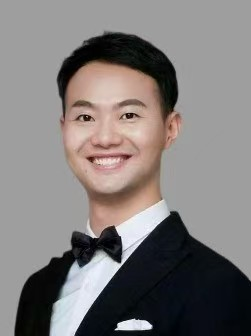
\includegraphics[width=1in,height=1.25in,clip,keepaspectratio]{fig2/Peng_Chen.png}}]{Peng Chen}
received the B.S. degree in information countermeasure technology and the Ph. D. degree in underwater acoustic engineering from Northwestern Polytechnical University (NWPU), Xi’an, China, in 2013, and 2019, respectively. From 2019 to 2024, he has worked as a postdoctoral fellow in civil engineering and wireless communication at Chang'an University, Xi’an, China. He is currently an associate professor with the School of Information Engineering, Chang'an University. His research interests include wireless channel modeling, localization, system design, and related topics. He received the Outstanding Doctoral Dissertation Award of Shaanxi Province, and of Chinese society of naval architecture and marine engineers (CSNAME) in 2021. He was honored as the Young Elite Scientists of the Acoustical Society of China (ASA) for his contribution in air-to-ground acoustic channel modeling and localization in 2024.
\end{IEEEbiography}

\begin{IEEEbiography}[{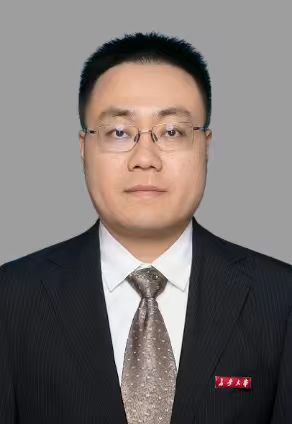
\includegraphics[width=1in,height=1.25in,clip,keepaspectratio]{fig2/Wei_Wang.png}}]{Wei Wang}
received the Bachelor degree in the field of communications engineering from University of Wuhan, China, in 2003 and the Master degree from University of Kiel, Germany, in 2006, and the Dr.-Ing. degree with summa cum laude from the University of Erlangen-Nuremberg, Germany in 2014. From 2007 to 2017, he worked as a scientific staff member at the Institute of Communications and Navigation of German Aerospace Center (DLR), Germany. Since 2018, he is a professor at Chang'an University. His research interests include channel characteristics analysis and modeling for localization/ navigation based on channel measurements, terrestrial radio based positioning/navigation and related topics. He coordinates several projects sponsored by NSFC, etc. and has participated in many projects sponsored by DLR, EU-FP6/7, and ESA, covering research studies in channel measurement, parameterization and modeling for indoor, airport, train, satellite and maritime propagation channel. He has authored or coauthored more than 150 publications in international journals and conferences. He received the Best Presentation/Paper Award in ION GNSS in 2012, best paper award in EUCAP in 2018, and IET Microwave Antennas \& Propagation Premium Award Winner in 2020.
\end{IEEEbiography}

\begin{IEEEbiography}[{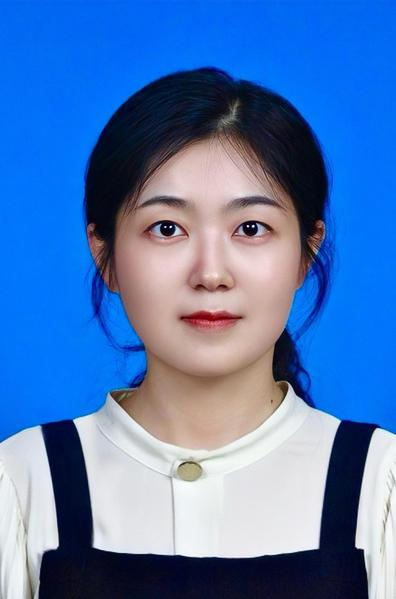
\includegraphics[width=1in,height=1.25in,clip,keepaspectratio]{fig2/Xin_Hu.png}}]{Xin Hu}
received the B.S. degree in ocean engineering from Harbin Engineering University, Harbin, China, in 2013, the M.S. degree and Ph.D. degree in underwater acoustics engineering from Northwestern Polytechnical University, Xi’an, China, in 2016 and 2023.
From 2022 to 2023, she was a Visiting Scholar with the Department of Electrical and Computer
Engineering, University of Victoria, BC, Canada. She is currently an assistant professor with the School of Future Transportation, Chang’an University, Xi’an China. Her research interest includes deep learning, underwater acoustic communication, acoustic signal processing algorithms, MIMO communication systems, and their applications.

\end{IEEEbiography}

\begin{IEEEbiography}[{
\includegraphics[width=1in,height=1.25in,clip,keepaspectratio]{fig2/Chentian_Xu.png}}]{Chentian Xu}
received the B.S. degree in underwater acoustics engineering from Northwestern Polytechnical University (NPU), Xi’an, China, in 2023, where he is currently working toward the Ph.D. degree in ship and ocean engineering. His research interests include underwater acoustic propagation in multi-scale dynamic environments, underwater target localization and signal processing.
\end{IEEEbiography}

\begin{IEEEbiography}[{
\includegraphics[width=1in,height=1.25in,clip,keepaspectratio]{fig2/Yang_Shi.png}}]{Yang Shi}
received the B.S. and M.S. degrees in electronic engineering and the Ph.D. degree in underwater acoustics engineering from Northwestern Polytechnical University, Xi’an, China in 2009, 2012, and 2017, respectively. From September 2017 to September 2020, he worked as a Post-Doctoral with the College of Oceanic and Atmospheric Science, Ocean University of China, Qingdao, China. Since September 2020, he has been working as a Full Professor with the School of Marine Science and Technology, Northwestern Polytechnical University. 
His research interests include ocean acoustic modeling, signal processing, and microwave propagation.
\end{IEEEbiography}


\end{document}


